\documentclass[11pt]{article}
\usepackage[margin=1in]{geometry}
\usepackage{graphicx}
\usepackage{amsmath}
\usepackage{amssymb}
\usepackage{xcolor}
\usepackage{caption}
\usepackage{array}     % needed for !{...} column separators
\usepackage{booktabs}
\usepackage{placeins}
\usepackage[hidelinks]{hyperref}

\graphicspath{{figures_enhanced/}}
\newcommand{\mpanel}[1]{\includegraphics[width=0.31\linewidth]{#1}}

\title{Results --- revised submission --- enhanced style}
\author{}
\date{}

\begin{document}
\maketitle

\section{Datasets}

\begin{table}[!htbp]
\centering
\begin{tabular}{l|l|r|r|r|r|r}
\hline
\# & Name & $N$ & $P$ & $K$ & MeanIR & CVIR \\
\hline
1 & GpositivePseAAC & 519 & 440 & 4 & 3.86 & 1.15 \\
2 & CHD\_49 & 555 & 49 & 6 & 5.77 & 1.60 \\
3 & Emotions & 593 & 72 & 6 & 1.48 & 0.16 \\
4 & Scene & 2407 & 294 & 6 & 1.25 & 0.11 \\
5 & PlantPseAAC & 978 & 440 & 12 & 6.69 & 0.68 \\
6 & Water-quality & 1060 & 16 & 14 & 1.77 & 0.29 \\
7 & Yeast & 2417 & 103 & 14 & 7.20 & 1.82 \\
8 & HumanPseAAC & 3106 & 440 & 14 & 15.29 & 1.05 \\
9 & enron & 1702 & 1001 & 53 & 10.45 & 0.80 \\
\hline
\end{tabular}
\caption{(Table 3) Datasets used in the revised experiments. $N$, $P$, $K$ are the number of instances, features, labels. MeanIR and CVIR report per-label imbalance (higher = more imbalanced).}
\label{tab:datasets_revised}
\end{table}

\section*{Pending follow-ups (to fill before final submission)}
\begin{itemize}
  \item \textbf{LGBM run on \texttt{enron}.} Sequentially training (~2--3h
        per task due to K=53 pairwise classifiers); will be merged into
        \texttt{full\_enron\_split\_lgbm\_summary/} when complete and the
        LGBM aggregate panels regenerated.
  \item \textbf{Extended PartialAbstention metrics.} The evaluator has been
        extended with 11 new PA metrics
        (\texttt{jaccard\_pa}, \texttt{\{example,macro,micro\}\_\{precision,recall,f1\}\_pa},
        \texttt{mfrd\_pa}, \texttt{afrd\_pa}). Existing runs were summarised
        with the previous metric set; the new columns will populate
        automatically on the next end-to-end training+evaluation pass.
\end{itemize}


\section{Method encoding}\label{sec:method_encoding}
For every panel that follows, the x-axis encodes the classifier as one of
12 methods, grouped into three blocks:

\paragraph{Block A --- Order-based predictors (ours, indices 1--8).}
Each name has the form \texttt{<order>-<target>-<height>}:
\emph{order} $\in$ \{PA = partial order, PR = pre-order\};
\emph{target} $\in$ \{H = Hamming, S = Subset~0/1\};
\emph{height} $\in$ \{2, $\infty$ (omitted in the label)\}.
\begin{itemize}
  \item 1\,=\,\textbf{PA-H-2}: partial order, Hamming target, height $\le 2$.
  \item 2\,=\,\textbf{PA-H}: partial order, Hamming target, unrestricted height.
  \item 3\,=\,\textbf{PA-S-2}: partial order, Subset 0/1 target, height $\le 2$.
  \item 4\,=\,\textbf{PA-S}: partial order, Subset 0/1, unrestricted.
  \item 5\,=\,\textbf{PR-H-2}: pre-order, Hamming, height $\le 2$.
  \item 6\,=\,\textbf{PR-H}: pre-order, Hamming, unrestricted.
  \item 7\,=\,\textbf{PR-S-2}: pre-order, Subset 0/1, height $\le 2$.
  \item 8\,=\,\textbf{PR-S}: pre-order, Subset 0/1, unrestricted.
\end{itemize}

\paragraph{Block B --- Standard MLC baselines from the original paper
(indices 9--11).}
\begin{itemize}
  \item 9\,=\,\textbf{BR} (Binary Relevance): $K$ independent binary
        classifiers, one per label.
  \item 10\,=\,\textbf{CC} (Classifier Chain): sequential chain that uses
        previous labels as features.
  \item 11\,=\,\textbf{CLR} (Calibrated Label Ranking): pairwise label
        ranking with a calibration label that separates relevant from
        irrelevant.
\end{itemize}

\paragraph{Block C --- Extended baseline added for the revision
(index 12).}
\begin{itemize}
  \item 12\,=\,\textbf{ECC} (Ensemble of Classifier Chains): averages over
        multiple CCs with random chain orders.
\end{itemize}

\paragraph{Reading the panels.} Each panel plots one dotted line with
markers per noise level. \textbf{Noise is encoded by warm-hue intensity}
(ColorBrewer YlOrRd): yellow $=$ clean ($\alpha=0.0$), dark red $=$ noisy
($\alpha=0.3$):
\textcolor[HTML]{fecc5c}{$\blacksquare$}\,$\alpha=0.0$,
\textcolor[HTML]{fd8d3c}{$\blacksquare$}\,$\alpha=0.1$,
\textcolor[HTML]{f03b20}{$\blacksquare$}\,$\alpha=0.2$,
\textcolor[HTML]{bd0026}{$\blacksquare$}\,$\alpha=0.3$.
Below the numeric x-axis (1--12), a second tier prints the short method
name so the reader can identify each classifier without referring back to
this section. \emph{PartialAbstention} and \emph{ScoreVector} panels show
only indices 1--8. A vertical dashed line at $x=8.5$ separates the
order-based block (1--8) from the standard MLC baselines (9--12). The
y-axis is zoomed to the actual data range to keep close-clustered curves
visually separable. Missing methods show as gaps in the line (with a
small grey ``x'' on the axis when the method has no data at all for that
panel).

\clearpage

\section{Paper results (RF base learner)}

Reproduces the layout of the original paper's main experiment tables (Tables~5--7): 3 datasets across, 4 metrics down, one table per prediction type (binary vector, partial abstention, score vector). Per the revision, $f^{\mathrm{ham}}_{\mathrm{MLC}}$ and $f^{\mathrm{sub}}_{\mathrm{MLC}}$ are dropped in favour of $f^{\mathrm{Jacc}}_{\mathrm{MLC}}$.


\pdfbookmark[2]{Table 3: Datasets}{paper-rf-datasets}

\begin{table}[!htbp]
\centering
\begin{tabular}{l|l|r|r|r|r|r}
\hline
\# & Name & $N$ & $P$ & $K$ & MeanIR & CVIR \\
\hline
1 & GpositivePseAAC & 519 & 440 & 4 & 3.86 & 1.15 \\
2 & CHD\_49 & 555 & 49 & 6 & 5.77 & 1.60 \\
3 & Emotions & 593 & 72 & 6 & 1.48 & 0.16 \\
4 & Scene & 2407 & 294 & 6 & 1.25 & 0.11 \\
5 & PlantPseAAC & 978 & 440 & 12 & 6.69 & 0.68 \\
6 & Water-quality & 1060 & 16 & 14 & 1.77 & 0.29 \\
7 & Yeast & 2417 & 103 & 14 & 7.20 & 1.82 \\
8 & HumanPseAAC & 3106 & 440 & 14 & 15.29 & 1.05 \\
9 & enron & 1702 & 1001 & 53 & 10.45 & 0.80 \\
\hline
\end{tabular}
\caption{(Table 3) Datasets used in the revised experiments. $N$, $P$, $K$ are the number of instances, features, labels. MeanIR and CVIR report per-label imbalance (higher = more imbalanced).}
\label{tab:datasets_revised}
\end{table}

\FloatBarrier

\subsection{Standard MLC predictions (BinaryVector)}

\pdfbookmark[3]{(Table 4) Group 1: GpositivePseAAC, PlantPseAAC, HumanPseAAC}{paper-rf-bv-g1}
\begin{table}[!htbp]
\centering
\setlength{\tabcolsep}{2pt}
\renewcommand{\arraystretch}{0.8}
\begin{tabular}{c!{\color{black!25}\vrule width 0.3pt}c!{\color{black!25}\vrule width 0.3pt}c}
\textbf{GpositivePse} & \textbf{plantPse} & \textbf{HumanPse} \\
\begin{minipage}{0.32\textwidth}\centering
\includegraphics[width=\linewidth]{rf/per_dataset/GpositivePseAAC/bv/f1_notitle.pdf}\\\scriptsize $f^{1}_{\mathrm{MLC}}$ (\ref{eq:f1mlc}) ($\uparrow$)\end{minipage} & \begin{minipage}{0.32\textwidth}\centering
\includegraphics[width=\linewidth]{rf/per_dataset/PlantPseAAC/bv/f1_notitle.pdf}\\\scriptsize $f^{1}_{\mathrm{MLC}}$ (\ref{eq:f1mlc}) ($\uparrow$)\end{minipage} & \begin{minipage}{0.32\textwidth}\centering
\includegraphics[width=\linewidth]{rf/per_dataset/HumanPseAAC/bv/f1_notitle.pdf}\\\scriptsize $f^{1}_{\mathrm{MLC}}$ (\ref{eq:f1mlc}) ($\uparrow$)\end{minipage} \\[6pt]
\begin{minipage}{0.32\textwidth}\centering
\includegraphics[width=\linewidth]{rf/per_dataset/GpositivePseAAC/bv/jaccard_notitle.pdf}\\\scriptsize $f^{\mathrm{Jacc}}_{\mathrm{MLC}}$ (\ref{eq:jaccmlc}) ($\uparrow$)\end{minipage} & \begin{minipage}{0.32\textwidth}\centering
\includegraphics[width=\linewidth]{rf/per_dataset/PlantPseAAC/bv/jaccard_notitle.pdf}\\\scriptsize $f^{\mathrm{Jacc}}_{\mathrm{MLC}}$ (\ref{eq:jaccmlc}) ($\uparrow$)\end{minipage} & \begin{minipage}{0.32\textwidth}\centering
\includegraphics[width=\linewidth]{rf/per_dataset/HumanPseAAC/bv/jaccard_notitle.pdf}\\\scriptsize $f^{\mathrm{Jacc}}_{\mathrm{MLC}}$ (\ref{eq:jaccmlc}) ($\uparrow$)\end{minipage} \\[6pt]
\begin{minipage}{0.32\textwidth}\centering
\includegraphics[width=\linewidth]{rf/per_dataset/GpositivePseAAC/bv/afrd_notitle.pdf}\\\scriptsize AFRD (\ref{eq:afrd}) ($\downarrow$)\end{minipage} & \begin{minipage}{0.32\textwidth}\centering
\includegraphics[width=\linewidth]{rf/per_dataset/PlantPseAAC/bv/afrd_notitle.pdf}\\\scriptsize AFRD (\ref{eq:afrd}) ($\downarrow$)\end{minipage} & \begin{minipage}{0.32\textwidth}\centering
\includegraphics[width=\linewidth]{rf/per_dataset/HumanPseAAC/bv/afrd_notitle.pdf}\\\scriptsize AFRD (\ref{eq:afrd}) ($\downarrow$)\end{minipage} \\[6pt]
\begin{minipage}{0.32\textwidth}\centering
\includegraphics[width=\linewidth]{rf/per_dataset/GpositivePseAAC/bv/mfrd_notitle.pdf}\\\scriptsize MFRD (\ref{eq:mfrd}) ($\downarrow$)\end{minipage} & \begin{minipage}{0.32\textwidth}\centering
\includegraphics[width=\linewidth]{rf/per_dataset/PlantPseAAC/bv/mfrd_notitle.pdf}\\\scriptsize MFRD (\ref{eq:mfrd}) ($\downarrow$)\end{minipage} & \begin{minipage}{0.32\textwidth}\centering
\includegraphics[width=\linewidth]{rf/per_dataset/HumanPseAAC/bv/mfrd_notitle.pdf}\\\scriptsize MFRD (\ref{eq:mfrd}) ($\downarrow$)\end{minipage} \\[6pt]
\end{tabular}
\caption{(Table 4) Average scores (in \%, $y$-axis) over $5\times 5$ cross-validation folds, plotted against the classifiers ($x$-axis): partial-order predictors (PA-H-2, PA-H, PA-S-2, PA-S), preorder predictors (PR-H-2, PR-H, PR-S-2, PR-S), and standard MLC baselines (BR, CC, CLR). Results are color-coded with respect to the noisy level $\alpha$ as follows: \textcolor[HTML]{fecc5c}{$\alpha = 0.0$}, \textcolor[HTML]{fd8d3c}{$\alpha = 0.1$}, \textcolor[HTML]{f03b20}{$\alpha = 0.2$} and \textcolor[HTML]{bd0026}{$\alpha = 0.3$}.}
\label{tab:paper_rf_bv_g1}
\end{table}

\FloatBarrier

\subsection{Partial abstention (PartialAbstention)}

\pdfbookmark[3]{(Table 5) Group 1: GpositivePseAAC, PlantPseAAC, HumanPseAAC}{paper-rf-pa-g1}
\begin{table}[!htbp]
\centering
\setlength{\tabcolsep}{2pt}
\renewcommand{\arraystretch}{0.8}
\begin{tabular}{c!{\color{black!25}\vrule width 0.3pt}c!{\color{black!25}\vrule width 0.3pt}c}
\textbf{GpositivePse} & \textbf{plantPse} & \textbf{HumanPse} \\
\begin{minipage}{0.32\textwidth}\centering
\includegraphics[width=\linewidth]{rf/per_dataset/GpositivePseAAC/pa/f1_pa_notitle.pdf}\\\scriptsize $f^{1}_{\mathrm{MLC}}$ (\ref{eq:f1mlc}) ($\uparrow$)\end{minipage} & \begin{minipage}{0.32\textwidth}\centering
\includegraphics[width=\linewidth]{rf/per_dataset/PlantPseAAC/pa/f1_pa_notitle.pdf}\\\scriptsize $f^{1}_{\mathrm{MLC}}$ (\ref{eq:f1mlc}) ($\uparrow$)\end{minipage} & \begin{minipage}{0.32\textwidth}\centering
\includegraphics[width=\linewidth]{rf/per_dataset/HumanPseAAC/pa/f1_pa_notitle.pdf}\\\scriptsize $f^{1}_{\mathrm{MLC}}$ (\ref{eq:f1mlc}) ($\uparrow$)\end{minipage} \\[6pt]
\begin{minipage}{0.32\textwidth}\centering
\includegraphics[width=\linewidth]{rf/per_dataset/GpositivePseAAC/pa/jaccard_pa_notitle.pdf}\\\scriptsize $f^{\mathrm{Jacc}}_{\mathrm{MLC}}$ (\ref{eq:jaccmlc}) ($\uparrow$)\end{minipage} & \begin{minipage}{0.32\textwidth}\centering
\includegraphics[width=\linewidth]{rf/per_dataset/PlantPseAAC/pa/jaccard_pa_notitle.pdf}\\\scriptsize $f^{\mathrm{Jacc}}_{\mathrm{MLC}}$ (\ref{eq:jaccmlc}) ($\uparrow$)\end{minipage} & \begin{minipage}{0.32\textwidth}\centering
\includegraphics[width=\linewidth]{rf/per_dataset/HumanPseAAC/pa/jaccard_pa_notitle.pdf}\\\scriptsize $f^{\mathrm{Jacc}}_{\mathrm{MLC}}$ (\ref{eq:jaccmlc}) ($\uparrow$)\end{minipage} \\[6pt]
\begin{minipage}{0.32\textwidth}\centering
\includegraphics[width=\linewidth]{rf/per_dataset/GpositivePseAAC/pa/aabs_notitle.pdf}\\\scriptsize $\mathrm{AABS}$ (\ref{eq:aabs}) ($\downarrow$)\end{minipage} & \begin{minipage}{0.32\textwidth}\centering
\includegraphics[width=\linewidth]{rf/per_dataset/PlantPseAAC/pa/aabs_notitle.pdf}\\\scriptsize $\mathrm{AABS}$ (\ref{eq:aabs}) ($\downarrow$)\end{minipage} & \begin{minipage}{0.32\textwidth}\centering
\includegraphics[width=\linewidth]{rf/per_dataset/HumanPseAAC/pa/aabs_notitle.pdf}\\\scriptsize $\mathrm{AABS}$ (\ref{eq:aabs}) ($\downarrow$)\end{minipage} \\[6pt]
\begin{minipage}{0.32\textwidth}\centering
\includegraphics[width=\linewidth]{rf/per_dataset/GpositivePseAAC/pa/abs_notitle.pdf}\\\scriptsize $\mathrm{ABS}$ (\ref{eq:abs}) ($\downarrow$)\end{minipage} & \begin{minipage}{0.32\textwidth}\centering
\includegraphics[width=\linewidth]{rf/per_dataset/PlantPseAAC/pa/abs_notitle.pdf}\\\scriptsize $\mathrm{ABS}$ (\ref{eq:abs}) ($\downarrow$)\end{minipage} & \begin{minipage}{0.32\textwidth}\centering
\includegraphics[width=\linewidth]{rf/per_dataset/HumanPseAAC/pa/abs_notitle.pdf}\\\scriptsize $\mathrm{ABS}$ (\ref{eq:abs}) ($\downarrow$)\end{minipage} \\[6pt]
\end{tabular}
\caption{(Table 5) Average scores (in \%, $y$-axis) over $5\times 5$ cross-validation folds, plotted against the classifiers ($x$-axis): partial-order predictors (PA-H-2, PA-H, PA-S-2, PA-S) and preorder predictors (PR-H-2, PR-H, PR-S-2, PR-S). Results are color-coded with respect to the noisy level $\alpha$ as follows: \textcolor[HTML]{fecc5c}{$\alpha = 0.0$}, \textcolor[HTML]{fd8d3c}{$\alpha = 0.1$}, \textcolor[HTML]{f03b20}{$\alpha = 0.2$} and \textcolor[HTML]{bd0026}{$\alpha = 0.3$}.}
\label{tab:paper_rf_pa_g1}
\end{table}

\FloatBarrier

\subsection{Experimental results --- appendix tables (RF base learner)}\label{sec:paperapp-rf}

Appendix counterpart of the main Paper results section. Tables All tables share the same 8-metric set (original 5 + 3 revision additions: $f^{\mathrm{Jacc}}_{\mathrm{MLC}}$, macro-$f_1$, micro-$f_1$). G2/G4 = imbalanced datasets, G3/G5 = balanced datasets (split follows the original paper's appendix). G6/G7 = main-paper datasets (GpositivePse, PlantPse, HumanPse) shown with the full metric set; the main body only carries the revised compact Tables 4/5.


\subsubsection{Standard MLC predictions (BinaryVector)}

\pdfbookmark[3]{(Table G2) Group 1: CHD_49, Yeast, enron}{paperapp_g2-rf-bv-g1}
\begin{table}[!htbp]
\centering
\setlength{\tabcolsep}{2pt}
\renewcommand{\arraystretch}{0.65}
\begin{tabular}{c!{\color{black!25}\vrule width 0.3pt}c!{\color{black!25}\vrule width 0.3pt}c}
\textbf{CHD-49} & \textbf{Yeast} & \textbf{enron} \\
\begin{minipage}{0.27\textwidth}\centering
\includegraphics[width=\linewidth]{rf/per_dataset/CHD_49/bv/f1_notitle.pdf}\\\scriptsize $f^{1}_{\mathrm{MLC}}$ (\ref{eq:f1mlc}) ($\uparrow$)\end{minipage} & \begin{minipage}{0.27\textwidth}\centering
\includegraphics[width=\linewidth]{rf/per_dataset/Yeast/bv/f1_notitle.pdf}\\\scriptsize $f^{1}_{\mathrm{MLC}}$ (\ref{eq:f1mlc}) ($\uparrow$)\end{minipage} & \begin{minipage}{0.27\textwidth}\centering
\includegraphics[width=\linewidth]{rf/per_dataset/enron/bv/f1_notitle.pdf}\\\scriptsize $f^{1}_{\mathrm{MLC}}$ (\ref{eq:f1mlc}) ($\uparrow$)\end{minipage} \\[8pt]
\begin{minipage}{0.27\textwidth}\centering
\includegraphics[width=\linewidth]{rf/per_dataset/CHD_49/bv/hamming_accuracy_notitle.pdf}\\\scriptsize $f^{\mathrm{ham}}_{\mathrm{MLC}}$ (\ref{eq:fham}) ($\uparrow$)\end{minipage} & \begin{minipage}{0.27\textwidth}\centering
\includegraphics[width=\linewidth]{rf/per_dataset/Yeast/bv/hamming_accuracy_notitle.pdf}\\\scriptsize $f^{\mathrm{ham}}_{\mathrm{MLC}}$ (\ref{eq:fham}) ($\uparrow$)\end{minipage} & \begin{minipage}{0.27\textwidth}\centering
\includegraphics[width=\linewidth]{rf/per_dataset/enron/bv/hamming_accuracy_notitle.pdf}\\\scriptsize $f^{\mathrm{ham}}_{\mathrm{MLC}}$ (\ref{eq:fham}) ($\uparrow$)\end{minipage} \\[8pt]
\begin{minipage}{0.27\textwidth}\centering
\includegraphics[width=\linewidth]{rf/per_dataset/CHD_49/bv/subset0_1_notitle.pdf}\\\scriptsize $f^{\mathrm{sub}}_{\mathrm{MLC}}$ (\ref{eq:fsub}) ($\uparrow$)\end{minipage} & \begin{minipage}{0.27\textwidth}\centering
\includegraphics[width=\linewidth]{rf/per_dataset/Yeast/bv/subset0_1_notitle.pdf}\\\scriptsize $f^{\mathrm{sub}}_{\mathrm{MLC}}$ (\ref{eq:fsub}) ($\uparrow$)\end{minipage} & \begin{minipage}{0.27\textwidth}\centering
\includegraphics[width=\linewidth]{rf/per_dataset/enron/bv/subset0_1_notitle.pdf}\\\scriptsize $f^{\mathrm{sub}}_{\mathrm{MLC}}$ (\ref{eq:fsub}) ($\uparrow$)\end{minipage} \\[8pt]
\begin{minipage}{0.27\textwidth}\centering
\includegraphics[width=\linewidth]{rf/per_dataset/CHD_49/bv/jaccard_notitle.pdf}\\\scriptsize $f^{\mathrm{Jacc}}_{\mathrm{MLC}}$ (\ref{eq:jaccmlc}) ($\uparrow$)\end{minipage} & \begin{minipage}{0.27\textwidth}\centering
\includegraphics[width=\linewidth]{rf/per_dataset/Yeast/bv/jaccard_notitle.pdf}\\\scriptsize $f^{\mathrm{Jacc}}_{\mathrm{MLC}}$ (\ref{eq:jaccmlc}) ($\uparrow$)\end{minipage} & \begin{minipage}{0.27\textwidth}\centering
\includegraphics[width=\linewidth]{rf/per_dataset/enron/bv/jaccard_notitle.pdf}\\\scriptsize $f^{\mathrm{Jacc}}_{\mathrm{MLC}}$ (\ref{eq:jaccmlc}) ($\uparrow$)\end{minipage} \\[8pt]
\begin{minipage}{0.27\textwidth}\centering
\includegraphics[width=\linewidth]{rf/per_dataset/CHD_49/bv/macro_f1_notitle.pdf}\\\scriptsize macro-$f_1$ (\ref{eq:macrof1}) ($\uparrow$)\end{minipage} & \begin{minipage}{0.27\textwidth}\centering
\includegraphics[width=\linewidth]{rf/per_dataset/Yeast/bv/macro_f1_notitle.pdf}\\\scriptsize macro-$f_1$ (\ref{eq:macrof1}) ($\uparrow$)\end{minipage} & \begin{minipage}{0.27\textwidth}\centering
\includegraphics[width=\linewidth]{rf/per_dataset/enron/bv/macro_f1_notitle.pdf}\\\scriptsize macro-$f_1$ (\ref{eq:macrof1}) ($\uparrow$)\end{minipage} \\[8pt]
\begin{minipage}{0.27\textwidth}\centering
\includegraphics[width=\linewidth]{rf/per_dataset/CHD_49/bv/micro_f1_notitle.pdf}\\\scriptsize micro-$f_1$ (\ref{eq:microf1}) ($\uparrow$)\end{minipage} & \begin{minipage}{0.27\textwidth}\centering
\includegraphics[width=\linewidth]{rf/per_dataset/Yeast/bv/micro_f1_notitle.pdf}\\\scriptsize micro-$f_1$ (\ref{eq:microf1}) ($\uparrow$)\end{minipage} & \begin{minipage}{0.27\textwidth}\centering
\includegraphics[width=\linewidth]{rf/per_dataset/enron/bv/micro_f1_notitle.pdf}\\\scriptsize micro-$f_1$ (\ref{eq:microf1}) ($\uparrow$)\end{minipage} \\[8pt]
\begin{minipage}{0.27\textwidth}\centering
\includegraphics[width=\linewidth]{rf/per_dataset/CHD_49/bv/afrd_notitle.pdf}\\\scriptsize AFRD (\ref{eq:afrd}) ($\downarrow$)\end{minipage} & \begin{minipage}{0.27\textwidth}\centering
\includegraphics[width=\linewidth]{rf/per_dataset/Yeast/bv/afrd_notitle.pdf}\\\scriptsize AFRD (\ref{eq:afrd}) ($\downarrow$)\end{minipage} & \begin{minipage}{0.27\textwidth}\centering
\includegraphics[width=\linewidth]{rf/per_dataset/enron/bv/afrd_notitle.pdf}\\\scriptsize AFRD (\ref{eq:afrd}) ($\downarrow$)\end{minipage} \\[8pt]
\begin{minipage}{0.27\textwidth}\centering
\includegraphics[width=\linewidth]{rf/per_dataset/CHD_49/bv/mfrd_notitle.pdf}\\\scriptsize MFRD (\ref{eq:mfrd}) ($\downarrow$)\end{minipage} & \begin{minipage}{0.27\textwidth}\centering
\includegraphics[width=\linewidth]{rf/per_dataset/Yeast/bv/mfrd_notitle.pdf}\\\scriptsize MFRD (\ref{eq:mfrd}) ($\downarrow$)\end{minipage} & \begin{minipage}{0.27\textwidth}\centering
\includegraphics[width=\linewidth]{rf/per_dataset/enron/bv/mfrd_notitle.pdf}\\\scriptsize MFRD (\ref{eq:mfrd}) ($\downarrow$)\end{minipage} \\[8pt]
\end{tabular}
\caption{(Table G2) Average scores (in \%, $y$-axis) over $5\times 5$ cross-validation folds, plotted against the classifiers ($x$-axis): partial-order predictors (PA-H-2, PA-H, PA-S-2, PA-S), preorder predictors (PR-H-2, PR-H, PR-S-2, PR-S), and standard MLC baselines (BR, CC, CLR). Results are color-coded with respect to the noisy level $\alpha$ as follows: \textcolor[HTML]{fecc5c}{$\alpha = 0.0$}, \textcolor[HTML]{fd8d3c}{$\alpha = 0.1$}, \textcolor[HTML]{f03b20}{$\alpha = 0.2$} and \textcolor[HTML]{bd0026}{$\alpha = 0.3$}.}
\label{tab:paperapp_g2_rf_bv_g1}
\end{table}

\FloatBarrier

\pdfbookmark[3]{(Table G3) Group 1: emotions, scene, Water-quality}{paperapp_g3-rf-bv-g1}
\begin{table}[!htbp]
\centering
\setlength{\tabcolsep}{2pt}
\renewcommand{\arraystretch}{0.65}
\begin{tabular}{c!{\color{black!25}\vrule width 0.3pt}c!{\color{black!25}\vrule width 0.3pt}c}
\textbf{emotions} & \textbf{scene} & \textbf{Water-quality} \\
\begin{minipage}{0.27\textwidth}\centering
\includegraphics[width=\linewidth]{rf/per_dataset/emotions/bv/f1_notitle.pdf}\\\scriptsize $f^{1}_{\mathrm{MLC}}$ (\ref{eq:f1mlc}) ($\uparrow$)\end{minipage} & \begin{minipage}{0.27\textwidth}\centering
\includegraphics[width=\linewidth]{rf/per_dataset/scene/bv/f1_notitle.pdf}\\\scriptsize $f^{1}_{\mathrm{MLC}}$ (\ref{eq:f1mlc}) ($\uparrow$)\end{minipage} & \begin{minipage}{0.27\textwidth}\centering
\includegraphics[width=\linewidth]{rf/per_dataset/Water-quality/bv/f1_notitle.pdf}\\\scriptsize $f^{1}_{\mathrm{MLC}}$ (\ref{eq:f1mlc}) ($\uparrow$)\end{minipage} \\[8pt]
\begin{minipage}{0.27\textwidth}\centering
\includegraphics[width=\linewidth]{rf/per_dataset/emotions/bv/hamming_accuracy_notitle.pdf}\\\scriptsize $f^{\mathrm{ham}}_{\mathrm{MLC}}$ (\ref{eq:fham}) ($\uparrow$)\end{minipage} & \begin{minipage}{0.27\textwidth}\centering
\includegraphics[width=\linewidth]{rf/per_dataset/scene/bv/hamming_accuracy_notitle.pdf}\\\scriptsize $f^{\mathrm{ham}}_{\mathrm{MLC}}$ (\ref{eq:fham}) ($\uparrow$)\end{minipage} & \begin{minipage}{0.27\textwidth}\centering
\includegraphics[width=\linewidth]{rf/per_dataset/Water-quality/bv/hamming_accuracy_notitle.pdf}\\\scriptsize $f^{\mathrm{ham}}_{\mathrm{MLC}}$ (\ref{eq:fham}) ($\uparrow$)\end{minipage} \\[8pt]
\begin{minipage}{0.27\textwidth}\centering
\includegraphics[width=\linewidth]{rf/per_dataset/emotions/bv/subset0_1_notitle.pdf}\\\scriptsize $f^{\mathrm{sub}}_{\mathrm{MLC}}$ (\ref{eq:fsub}) ($\uparrow$)\end{minipage} & \begin{minipage}{0.27\textwidth}\centering
\includegraphics[width=\linewidth]{rf/per_dataset/scene/bv/subset0_1_notitle.pdf}\\\scriptsize $f^{\mathrm{sub}}_{\mathrm{MLC}}$ (\ref{eq:fsub}) ($\uparrow$)\end{minipage} & \begin{minipage}{0.27\textwidth}\centering
\includegraphics[width=\linewidth]{rf/per_dataset/Water-quality/bv/subset0_1_notitle.pdf}\\\scriptsize $f^{\mathrm{sub}}_{\mathrm{MLC}}$ (\ref{eq:fsub}) ($\uparrow$)\end{minipage} \\[8pt]
\begin{minipage}{0.27\textwidth}\centering
\includegraphics[width=\linewidth]{rf/per_dataset/emotions/bv/jaccard_notitle.pdf}\\\scriptsize $f^{\mathrm{Jacc}}_{\mathrm{MLC}}$ (\ref{eq:jaccmlc}) ($\uparrow$)\end{minipage} & \begin{minipage}{0.27\textwidth}\centering
\includegraphics[width=\linewidth]{rf/per_dataset/scene/bv/jaccard_notitle.pdf}\\\scriptsize $f^{\mathrm{Jacc}}_{\mathrm{MLC}}$ (\ref{eq:jaccmlc}) ($\uparrow$)\end{minipage} & \begin{minipage}{0.27\textwidth}\centering
\includegraphics[width=\linewidth]{rf/per_dataset/Water-quality/bv/jaccard_notitle.pdf}\\\scriptsize $f^{\mathrm{Jacc}}_{\mathrm{MLC}}$ (\ref{eq:jaccmlc}) ($\uparrow$)\end{minipage} \\[8pt]
\begin{minipage}{0.27\textwidth}\centering
\includegraphics[width=\linewidth]{rf/per_dataset/emotions/bv/macro_f1_notitle.pdf}\\\scriptsize macro-$f_1$ (\ref{eq:macrof1}) ($\uparrow$)\end{minipage} & \begin{minipage}{0.27\textwidth}\centering
\includegraphics[width=\linewidth]{rf/per_dataset/scene/bv/macro_f1_notitle.pdf}\\\scriptsize macro-$f_1$ (\ref{eq:macrof1}) ($\uparrow$)\end{minipage} & \begin{minipage}{0.27\textwidth}\centering
\includegraphics[width=\linewidth]{rf/per_dataset/Water-quality/bv/macro_f1_notitle.pdf}\\\scriptsize macro-$f_1$ (\ref{eq:macrof1}) ($\uparrow$)\end{minipage} \\[8pt]
\begin{minipage}{0.27\textwidth}\centering
\includegraphics[width=\linewidth]{rf/per_dataset/emotions/bv/micro_f1_notitle.pdf}\\\scriptsize micro-$f_1$ (\ref{eq:microf1}) ($\uparrow$)\end{minipage} & \begin{minipage}{0.27\textwidth}\centering
\includegraphics[width=\linewidth]{rf/per_dataset/scene/bv/micro_f1_notitle.pdf}\\\scriptsize micro-$f_1$ (\ref{eq:microf1}) ($\uparrow$)\end{minipage} & \begin{minipage}{0.27\textwidth}\centering
\includegraphics[width=\linewidth]{rf/per_dataset/Water-quality/bv/micro_f1_notitle.pdf}\\\scriptsize micro-$f_1$ (\ref{eq:microf1}) ($\uparrow$)\end{minipage} \\[8pt]
\begin{minipage}{0.27\textwidth}\centering
\includegraphics[width=\linewidth]{rf/per_dataset/emotions/bv/afrd_notitle.pdf}\\\scriptsize AFRD (\ref{eq:afrd}) ($\downarrow$)\end{minipage} & \begin{minipage}{0.27\textwidth}\centering
\includegraphics[width=\linewidth]{rf/per_dataset/scene/bv/afrd_notitle.pdf}\\\scriptsize AFRD (\ref{eq:afrd}) ($\downarrow$)\end{minipage} & \begin{minipage}{0.27\textwidth}\centering
\includegraphics[width=\linewidth]{rf/per_dataset/Water-quality/bv/afrd_notitle.pdf}\\\scriptsize AFRD (\ref{eq:afrd}) ($\downarrow$)\end{minipage} \\[8pt]
\begin{minipage}{0.27\textwidth}\centering
\includegraphics[width=\linewidth]{rf/per_dataset/emotions/bv/mfrd_notitle.pdf}\\\scriptsize MFRD (\ref{eq:mfrd}) ($\downarrow$)\end{minipage} & \begin{minipage}{0.27\textwidth}\centering
\includegraphics[width=\linewidth]{rf/per_dataset/scene/bv/mfrd_notitle.pdf}\\\scriptsize MFRD (\ref{eq:mfrd}) ($\downarrow$)\end{minipage} & \begin{minipage}{0.27\textwidth}\centering
\includegraphics[width=\linewidth]{rf/per_dataset/Water-quality/bv/mfrd_notitle.pdf}\\\scriptsize MFRD (\ref{eq:mfrd}) ($\downarrow$)\end{minipage} \\[8pt]
\end{tabular}
\caption{(Table G3) Average scores (in \%, $y$-axis) over $5\times 5$ cross-validation folds, plotted against the classifiers ($x$-axis): partial-order predictors (PA-H-2, PA-H, PA-S-2, PA-S), preorder predictors (PR-H-2, PR-H, PR-S-2, PR-S), and standard MLC baselines (BR, CC, CLR). Results are color-coded with respect to the noisy level $\alpha$ as follows: \textcolor[HTML]{fecc5c}{$\alpha = 0.0$}, \textcolor[HTML]{fd8d3c}{$\alpha = 0.1$}, \textcolor[HTML]{f03b20}{$\alpha = 0.2$} and \textcolor[HTML]{bd0026}{$\alpha = 0.3$}.}
\label{tab:paperapp_g3_rf_bv_g1}
\end{table}

\FloatBarrier

\subsubsection{Partial abstention (PartialAbstention)}

\pdfbookmark[3]{(Table G4) Group 1: CHD_49, Yeast, enron}{paperapp_g4-rf-pa-g1}
\begin{table}[!htbp]
\centering
\setlength{\tabcolsep}{2pt}
\renewcommand{\arraystretch}{0.65}
\begin{tabular}{c!{\color{black!25}\vrule width 0.3pt}c!{\color{black!25}\vrule width 0.3pt}c}
\textbf{CHD-49} & \textbf{Yeast} & \textbf{enron} \\
\begin{minipage}{0.27\textwidth}\centering
\includegraphics[width=\linewidth]{rf/per_dataset/CHD_49/pa/f1_pa_notitle.pdf}\\\scriptsize $f^{1}_{\mathrm{MLC}}$ (\ref{eq:f1mlc}) ($\uparrow$)\end{minipage} & \begin{minipage}{0.27\textwidth}\centering
\includegraphics[width=\linewidth]{rf/per_dataset/Yeast/pa/f1_pa_notitle.pdf}\\\scriptsize $f^{1}_{\mathrm{MLC}}$ (\ref{eq:f1mlc}) ($\uparrow$)\end{minipage} & \begin{minipage}{0.27\textwidth}\centering
\includegraphics[width=\linewidth]{rf/per_dataset/enron/pa/f1_pa_notitle.pdf}\\\scriptsize $f^{1}_{\mathrm{MLC}}$ (\ref{eq:f1mlc}) ($\uparrow$)\end{minipage} \\[8pt]
\begin{minipage}{0.27\textwidth}\centering
\includegraphics[width=\linewidth]{rf/per_dataset/CHD_49/pa/hamming_accuracy_pa_notitle.pdf}\\\scriptsize $f^{\mathrm{ham}}_{\mathrm{MLC}}$ (\ref{eq:fham}) ($\uparrow$)\end{minipage} & \begin{minipage}{0.27\textwidth}\centering
\includegraphics[width=\linewidth]{rf/per_dataset/Yeast/pa/hamming_accuracy_pa_notitle.pdf}\\\scriptsize $f^{\mathrm{ham}}_{\mathrm{MLC}}$ (\ref{eq:fham}) ($\uparrow$)\end{minipage} & \begin{minipage}{0.27\textwidth}\centering
\includegraphics[width=\linewidth]{rf/per_dataset/enron/pa/hamming_accuracy_pa_notitle.pdf}\\\scriptsize $f^{\mathrm{ham}}_{\mathrm{MLC}}$ (\ref{eq:fham}) ($\uparrow$)\end{minipage} \\[8pt]
\begin{minipage}{0.27\textwidth}\centering
\includegraphics[width=\linewidth]{rf/per_dataset/CHD_49/pa/subset0_1_pa_notitle.pdf}\\\scriptsize $f^{\mathrm{sub}}_{\mathrm{MLC}}$ (\ref{eq:fsub}) ($\uparrow$)\end{minipage} & \begin{minipage}{0.27\textwidth}\centering
\includegraphics[width=\linewidth]{rf/per_dataset/Yeast/pa/subset0_1_pa_notitle.pdf}\\\scriptsize $f^{\mathrm{sub}}_{\mathrm{MLC}}$ (\ref{eq:fsub}) ($\uparrow$)\end{minipage} & \begin{minipage}{0.27\textwidth}\centering
\includegraphics[width=\linewidth]{rf/per_dataset/enron/pa/subset0_1_pa_notitle.pdf}\\\scriptsize $f^{\mathrm{sub}}_{\mathrm{MLC}}$ (\ref{eq:fsub}) ($\uparrow$)\end{minipage} \\[8pt]
\begin{minipage}{0.27\textwidth}\centering
\includegraphics[width=\linewidth]{rf/per_dataset/CHD_49/pa/jaccard_pa_notitle.pdf}\\\scriptsize $f^{\mathrm{Jacc}}_{\mathrm{MLC}}$ (\ref{eq:jaccmlc}) ($\uparrow$)\end{minipage} & \begin{minipage}{0.27\textwidth}\centering
\includegraphics[width=\linewidth]{rf/per_dataset/Yeast/pa/jaccard_pa_notitle.pdf}\\\scriptsize $f^{\mathrm{Jacc}}_{\mathrm{MLC}}$ (\ref{eq:jaccmlc}) ($\uparrow$)\end{minipage} & \begin{minipage}{0.27\textwidth}\centering
\includegraphics[width=\linewidth]{rf/per_dataset/enron/pa/jaccard_pa_notitle.pdf}\\\scriptsize $f^{\mathrm{Jacc}}_{\mathrm{MLC}}$ (\ref{eq:jaccmlc}) ($\uparrow$)\end{minipage} \\[8pt]
\begin{minipage}{0.27\textwidth}\centering
\includegraphics[width=\linewidth]{rf/per_dataset/CHD_49/pa/macro_f1_pa_notitle.pdf}\\\scriptsize macro-$f_1$ (\ref{eq:macrof1}) ($\uparrow$)\end{minipage} & \begin{minipage}{0.27\textwidth}\centering
\includegraphics[width=\linewidth]{rf/per_dataset/Yeast/pa/macro_f1_pa_notitle.pdf}\\\scriptsize macro-$f_1$ (\ref{eq:macrof1}) ($\uparrow$)\end{minipage} & \begin{minipage}{0.27\textwidth}\centering
\includegraphics[width=\linewidth]{rf/per_dataset/enron/pa/macro_f1_pa_notitle.pdf}\\\scriptsize macro-$f_1$ (\ref{eq:macrof1}) ($\uparrow$)\end{minipage} \\[8pt]
\begin{minipage}{0.27\textwidth}\centering
\includegraphics[width=\linewidth]{rf/per_dataset/CHD_49/pa/micro_f1_pa_notitle.pdf}\\\scriptsize micro-$f_1$ (\ref{eq:microf1}) ($\uparrow$)\end{minipage} & \begin{minipage}{0.27\textwidth}\centering
\includegraphics[width=\linewidth]{rf/per_dataset/Yeast/pa/micro_f1_pa_notitle.pdf}\\\scriptsize micro-$f_1$ (\ref{eq:microf1}) ($\uparrow$)\end{minipage} & \begin{minipage}{0.27\textwidth}\centering
\includegraphics[width=\linewidth]{rf/per_dataset/enron/pa/micro_f1_pa_notitle.pdf}\\\scriptsize micro-$f_1$ (\ref{eq:microf1}) ($\uparrow$)\end{minipage} \\[8pt]
\begin{minipage}{0.27\textwidth}\centering
\includegraphics[width=\linewidth]{rf/per_dataset/CHD_49/pa/aabs_notitle.pdf}\\\scriptsize AABS (\ref{eq:aabs}) ($\downarrow$)\end{minipage} & \begin{minipage}{0.27\textwidth}\centering
\includegraphics[width=\linewidth]{rf/per_dataset/Yeast/pa/aabs_notitle.pdf}\\\scriptsize AABS (\ref{eq:aabs}) ($\downarrow$)\end{minipage} & \begin{minipage}{0.27\textwidth}\centering
\includegraphics[width=\linewidth]{rf/per_dataset/enron/pa/aabs_notitle.pdf}\\\scriptsize AABS (\ref{eq:aabs}) ($\downarrow$)\end{minipage} \\[8pt]
\begin{minipage}{0.27\textwidth}\centering
\includegraphics[width=\linewidth]{rf/per_dataset/CHD_49/pa/abs_notitle.pdf}\\\scriptsize ABS (\ref{eq:abs}) ($\downarrow$)\end{minipage} & \begin{minipage}{0.27\textwidth}\centering
\includegraphics[width=\linewidth]{rf/per_dataset/Yeast/pa/abs_notitle.pdf}\\\scriptsize ABS (\ref{eq:abs}) ($\downarrow$)\end{minipage} & \begin{minipage}{0.27\textwidth}\centering
\includegraphics[width=\linewidth]{rf/per_dataset/enron/pa/abs_notitle.pdf}\\\scriptsize ABS (\ref{eq:abs}) ($\downarrow$)\end{minipage} \\[8pt]
\end{tabular}
\caption{(Table G4) Average scores (in \%, $y$-axis) over $5\times 5$ cross-validation folds, plotted against the classifiers ($x$-axis): partial-order predictors (PA-H-2, PA-H, PA-S-2, PA-S) and preorder predictors (PR-H-2, PR-H, PR-S-2, PR-S). Results are color-coded with respect to the noisy level $\alpha$ as follows: \textcolor[HTML]{fecc5c}{$\alpha = 0.0$}, \textcolor[HTML]{fd8d3c}{$\alpha = 0.1$}, \textcolor[HTML]{f03b20}{$\alpha = 0.2$} and \textcolor[HTML]{bd0026}{$\alpha = 0.3$}.}
\label{tab:paperapp_g4_rf_pa_g1}
\end{table}

\FloatBarrier

\pdfbookmark[3]{(Table G5) Group 1: emotions, scene, Water-quality}{paperapp_g5-rf-pa-g1}
\begin{table}[!htbp]
\centering
\setlength{\tabcolsep}{2pt}
\renewcommand{\arraystretch}{0.65}
\begin{tabular}{c!{\color{black!25}\vrule width 0.3pt}c!{\color{black!25}\vrule width 0.3pt}c}
\textbf{emotions} & \textbf{scene} & \textbf{Water-quality} \\
\begin{minipage}{0.27\textwidth}\centering
\includegraphics[width=\linewidth]{rf/per_dataset/emotions/pa/f1_pa_notitle.pdf}\\\scriptsize $f^{1}_{\mathrm{MLC}}$ (\ref{eq:f1mlc}) ($\uparrow$)\end{minipage} & \begin{minipage}{0.27\textwidth}\centering
\includegraphics[width=\linewidth]{rf/per_dataset/scene/pa/f1_pa_notitle.pdf}\\\scriptsize $f^{1}_{\mathrm{MLC}}$ (\ref{eq:f1mlc}) ($\uparrow$)\end{minipage} & \begin{minipage}{0.27\textwidth}\centering
\includegraphics[width=\linewidth]{rf/per_dataset/Water-quality/pa/f1_pa_notitle.pdf}\\\scriptsize $f^{1}_{\mathrm{MLC}}$ (\ref{eq:f1mlc}) ($\uparrow$)\end{minipage} \\[8pt]
\begin{minipage}{0.27\textwidth}\centering
\includegraphics[width=\linewidth]{rf/per_dataset/emotions/pa/hamming_accuracy_pa_notitle.pdf}\\\scriptsize $f^{\mathrm{ham}}_{\mathrm{MLC}}$ (\ref{eq:fham}) ($\uparrow$)\end{minipage} & \begin{minipage}{0.27\textwidth}\centering
\includegraphics[width=\linewidth]{rf/per_dataset/scene/pa/hamming_accuracy_pa_notitle.pdf}\\\scriptsize $f^{\mathrm{ham}}_{\mathrm{MLC}}$ (\ref{eq:fham}) ($\uparrow$)\end{minipage} & \begin{minipage}{0.27\textwidth}\centering
\includegraphics[width=\linewidth]{rf/per_dataset/Water-quality/pa/hamming_accuracy_pa_notitle.pdf}\\\scriptsize $f^{\mathrm{ham}}_{\mathrm{MLC}}$ (\ref{eq:fham}) ($\uparrow$)\end{minipage} \\[8pt]
\begin{minipage}{0.27\textwidth}\centering
\includegraphics[width=\linewidth]{rf/per_dataset/emotions/pa/subset0_1_pa_notitle.pdf}\\\scriptsize $f^{\mathrm{sub}}_{\mathrm{MLC}}$ (\ref{eq:fsub}) ($\uparrow$)\end{minipage} & \begin{minipage}{0.27\textwidth}\centering
\includegraphics[width=\linewidth]{rf/per_dataset/scene/pa/subset0_1_pa_notitle.pdf}\\\scriptsize $f^{\mathrm{sub}}_{\mathrm{MLC}}$ (\ref{eq:fsub}) ($\uparrow$)\end{minipage} & \begin{minipage}{0.27\textwidth}\centering
\includegraphics[width=\linewidth]{rf/per_dataset/Water-quality/pa/subset0_1_pa_notitle.pdf}\\\scriptsize $f^{\mathrm{sub}}_{\mathrm{MLC}}$ (\ref{eq:fsub}) ($\uparrow$)\end{minipage} \\[8pt]
\begin{minipage}{0.27\textwidth}\centering
\includegraphics[width=\linewidth]{rf/per_dataset/emotions/pa/jaccard_pa_notitle.pdf}\\\scriptsize $f^{\mathrm{Jacc}}_{\mathrm{MLC}}$ (\ref{eq:jaccmlc}) ($\uparrow$)\end{minipage} & \begin{minipage}{0.27\textwidth}\centering
\includegraphics[width=\linewidth]{rf/per_dataset/scene/pa/jaccard_pa_notitle.pdf}\\\scriptsize $f^{\mathrm{Jacc}}_{\mathrm{MLC}}$ (\ref{eq:jaccmlc}) ($\uparrow$)\end{minipage} & \begin{minipage}{0.27\textwidth}\centering
\includegraphics[width=\linewidth]{rf/per_dataset/Water-quality/pa/jaccard_pa_notitle.pdf}\\\scriptsize $f^{\mathrm{Jacc}}_{\mathrm{MLC}}$ (\ref{eq:jaccmlc}) ($\uparrow$)\end{minipage} \\[8pt]
\begin{minipage}{0.27\textwidth}\centering
\includegraphics[width=\linewidth]{rf/per_dataset/emotions/pa/macro_f1_pa_notitle.pdf}\\\scriptsize macro-$f_1$ (\ref{eq:macrof1}) ($\uparrow$)\end{minipage} & \begin{minipage}{0.27\textwidth}\centering
\includegraphics[width=\linewidth]{rf/per_dataset/scene/pa/macro_f1_pa_notitle.pdf}\\\scriptsize macro-$f_1$ (\ref{eq:macrof1}) ($\uparrow$)\end{minipage} & \begin{minipage}{0.27\textwidth}\centering
\includegraphics[width=\linewidth]{rf/per_dataset/Water-quality/pa/macro_f1_pa_notitle.pdf}\\\scriptsize macro-$f_1$ (\ref{eq:macrof1}) ($\uparrow$)\end{minipage} \\[8pt]
\begin{minipage}{0.27\textwidth}\centering
\includegraphics[width=\linewidth]{rf/per_dataset/emotions/pa/micro_f1_pa_notitle.pdf}\\\scriptsize micro-$f_1$ (\ref{eq:microf1}) ($\uparrow$)\end{minipage} & \begin{minipage}{0.27\textwidth}\centering
\includegraphics[width=\linewidth]{rf/per_dataset/scene/pa/micro_f1_pa_notitle.pdf}\\\scriptsize micro-$f_1$ (\ref{eq:microf1}) ($\uparrow$)\end{minipage} & \begin{minipage}{0.27\textwidth}\centering
\includegraphics[width=\linewidth]{rf/per_dataset/Water-quality/pa/micro_f1_pa_notitle.pdf}\\\scriptsize micro-$f_1$ (\ref{eq:microf1}) ($\uparrow$)\end{minipage} \\[8pt]
\begin{minipage}{0.27\textwidth}\centering
\includegraphics[width=\linewidth]{rf/per_dataset/emotions/pa/aabs_notitle.pdf}\\\scriptsize AABS (\ref{eq:aabs}) ($\downarrow$)\end{minipage} & \begin{minipage}{0.27\textwidth}\centering
\includegraphics[width=\linewidth]{rf/per_dataset/scene/pa/aabs_notitle.pdf}\\\scriptsize AABS (\ref{eq:aabs}) ($\downarrow$)\end{minipage} & \begin{minipage}{0.27\textwidth}\centering
\includegraphics[width=\linewidth]{rf/per_dataset/Water-quality/pa/aabs_notitle.pdf}\\\scriptsize AABS (\ref{eq:aabs}) ($\downarrow$)\end{minipage} \\[8pt]
\begin{minipage}{0.27\textwidth}\centering
\includegraphics[width=\linewidth]{rf/per_dataset/emotions/pa/abs_notitle.pdf}\\\scriptsize ABS (\ref{eq:abs}) ($\downarrow$)\end{minipage} & \begin{minipage}{0.27\textwidth}\centering
\includegraphics[width=\linewidth]{rf/per_dataset/scene/pa/abs_notitle.pdf}\\\scriptsize ABS (\ref{eq:abs}) ($\downarrow$)\end{minipage} & \begin{minipage}{0.27\textwidth}\centering
\includegraphics[width=\linewidth]{rf/per_dataset/Water-quality/pa/abs_notitle.pdf}\\\scriptsize ABS (\ref{eq:abs}) ($\downarrow$)\end{minipage} \\[8pt]
\end{tabular}
\caption{(Table G5) Average scores (in \%, $y$-axis) over $5\times 5$ cross-validation folds, plotted against the classifiers ($x$-axis): partial-order predictors (PA-H-2, PA-H, PA-S-2, PA-S) and preorder predictors (PR-H-2, PR-H, PR-S-2, PR-S). Results are color-coded with respect to the noisy level $\alpha$ as follows: \textcolor[HTML]{fecc5c}{$\alpha = 0.0$}, \textcolor[HTML]{fd8d3c}{$\alpha = 0.1$}, \textcolor[HTML]{f03b20}{$\alpha = 0.2$} and \textcolor[HTML]{bd0026}{$\alpha = 0.3$}.}
\label{tab:paperapp_g5_rf_pa_g1}
\end{table}

\FloatBarrier

\subsubsection{Standard MLC predictions (BinaryVector)}

\pdfbookmark[3]{(Table G6) Group 1: GpositivePseAAC, PlantPseAAC, HumanPseAAC}{paperapp_g6-rf-bv-g1}
\begin{table}[!htbp]
\centering
\setlength{\tabcolsep}{2pt}
\renewcommand{\arraystretch}{0.65}
\begin{tabular}{c!{\color{black!25}\vrule width 0.3pt}c!{\color{black!25}\vrule width 0.3pt}c}
\textbf{GpositivePse} & \textbf{plantPse} & \textbf{HumanPse} \\
\begin{minipage}{0.27\textwidth}\centering
\includegraphics[width=\linewidth]{rf/per_dataset/GpositivePseAAC/bv/f1_notitle.pdf}\\\scriptsize $f^{1}_{\mathrm{MLC}}$ (\ref{eq:f1mlc}) ($\uparrow$)\end{minipage} & \begin{minipage}{0.27\textwidth}\centering
\includegraphics[width=\linewidth]{rf/per_dataset/PlantPseAAC/bv/f1_notitle.pdf}\\\scriptsize $f^{1}_{\mathrm{MLC}}$ (\ref{eq:f1mlc}) ($\uparrow$)\end{minipage} & \begin{minipage}{0.27\textwidth}\centering
\includegraphics[width=\linewidth]{rf/per_dataset/HumanPseAAC/bv/f1_notitle.pdf}\\\scriptsize $f^{1}_{\mathrm{MLC}}$ (\ref{eq:f1mlc}) ($\uparrow$)\end{minipage} \\[8pt]
\begin{minipage}{0.27\textwidth}\centering
\includegraphics[width=\linewidth]{rf/per_dataset/GpositivePseAAC/bv/hamming_accuracy_notitle.pdf}\\\scriptsize $f^{\mathrm{ham}}_{\mathrm{MLC}}$ (\ref{eq:fham}) ($\uparrow$)\end{minipage} & \begin{minipage}{0.27\textwidth}\centering
\includegraphics[width=\linewidth]{rf/per_dataset/PlantPseAAC/bv/hamming_accuracy_notitle.pdf}\\\scriptsize $f^{\mathrm{ham}}_{\mathrm{MLC}}$ (\ref{eq:fham}) ($\uparrow$)\end{minipage} & \begin{minipage}{0.27\textwidth}\centering
\includegraphics[width=\linewidth]{rf/per_dataset/HumanPseAAC/bv/hamming_accuracy_notitle.pdf}\\\scriptsize $f^{\mathrm{ham}}_{\mathrm{MLC}}$ (\ref{eq:fham}) ($\uparrow$)\end{minipage} \\[8pt]
\begin{minipage}{0.27\textwidth}\centering
\includegraphics[width=\linewidth]{rf/per_dataset/GpositivePseAAC/bv/subset0_1_notitle.pdf}\\\scriptsize $f^{\mathrm{sub}}_{\mathrm{MLC}}$ (\ref{eq:fsub}) ($\uparrow$)\end{minipage} & \begin{minipage}{0.27\textwidth}\centering
\includegraphics[width=\linewidth]{rf/per_dataset/PlantPseAAC/bv/subset0_1_notitle.pdf}\\\scriptsize $f^{\mathrm{sub}}_{\mathrm{MLC}}$ (\ref{eq:fsub}) ($\uparrow$)\end{minipage} & \begin{minipage}{0.27\textwidth}\centering
\includegraphics[width=\linewidth]{rf/per_dataset/HumanPseAAC/bv/subset0_1_notitle.pdf}\\\scriptsize $f^{\mathrm{sub}}_{\mathrm{MLC}}$ (\ref{eq:fsub}) ($\uparrow$)\end{minipage} \\[8pt]
\begin{minipage}{0.27\textwidth}\centering
\includegraphics[width=\linewidth]{rf/per_dataset/GpositivePseAAC/bv/jaccard_notitle.pdf}\\\scriptsize $f^{\mathrm{Jacc}}_{\mathrm{MLC}}$ (\ref{eq:jaccmlc}) ($\uparrow$)\end{minipage} & \begin{minipage}{0.27\textwidth}\centering
\includegraphics[width=\linewidth]{rf/per_dataset/PlantPseAAC/bv/jaccard_notitle.pdf}\\\scriptsize $f^{\mathrm{Jacc}}_{\mathrm{MLC}}$ (\ref{eq:jaccmlc}) ($\uparrow$)\end{minipage} & \begin{minipage}{0.27\textwidth}\centering
\includegraphics[width=\linewidth]{rf/per_dataset/HumanPseAAC/bv/jaccard_notitle.pdf}\\\scriptsize $f^{\mathrm{Jacc}}_{\mathrm{MLC}}$ (\ref{eq:jaccmlc}) ($\uparrow$)\end{minipage} \\[8pt]
\begin{minipage}{0.27\textwidth}\centering
\includegraphics[width=\linewidth]{rf/per_dataset/GpositivePseAAC/bv/macro_f1_notitle.pdf}\\\scriptsize macro-$f_1$ (\ref{eq:macrof1}) ($\uparrow$)\end{minipage} & \begin{minipage}{0.27\textwidth}\centering
\includegraphics[width=\linewidth]{rf/per_dataset/PlantPseAAC/bv/macro_f1_notitle.pdf}\\\scriptsize macro-$f_1$ (\ref{eq:macrof1}) ($\uparrow$)\end{minipage} & \begin{minipage}{0.27\textwidth}\centering
\includegraphics[width=\linewidth]{rf/per_dataset/HumanPseAAC/bv/macro_f1_notitle.pdf}\\\scriptsize macro-$f_1$ (\ref{eq:macrof1}) ($\uparrow$)\end{minipage} \\[8pt]
\begin{minipage}{0.27\textwidth}\centering
\includegraphics[width=\linewidth]{rf/per_dataset/GpositivePseAAC/bv/micro_f1_notitle.pdf}\\\scriptsize micro-$f_1$ (\ref{eq:microf1}) ($\uparrow$)\end{minipage} & \begin{minipage}{0.27\textwidth}\centering
\includegraphics[width=\linewidth]{rf/per_dataset/PlantPseAAC/bv/micro_f1_notitle.pdf}\\\scriptsize micro-$f_1$ (\ref{eq:microf1}) ($\uparrow$)\end{minipage} & \begin{minipage}{0.27\textwidth}\centering
\includegraphics[width=\linewidth]{rf/per_dataset/HumanPseAAC/bv/micro_f1_notitle.pdf}\\\scriptsize micro-$f_1$ (\ref{eq:microf1}) ($\uparrow$)\end{minipage} \\[8pt]
\begin{minipage}{0.27\textwidth}\centering
\includegraphics[width=\linewidth]{rf/per_dataset/GpositivePseAAC/bv/afrd_notitle.pdf}\\\scriptsize AFRD (\ref{eq:afrd}) ($\downarrow$)\end{minipage} & \begin{minipage}{0.27\textwidth}\centering
\includegraphics[width=\linewidth]{rf/per_dataset/PlantPseAAC/bv/afrd_notitle.pdf}\\\scriptsize AFRD (\ref{eq:afrd}) ($\downarrow$)\end{minipage} & \begin{minipage}{0.27\textwidth}\centering
\includegraphics[width=\linewidth]{rf/per_dataset/HumanPseAAC/bv/afrd_notitle.pdf}\\\scriptsize AFRD (\ref{eq:afrd}) ($\downarrow$)\end{minipage} \\[8pt]
\begin{minipage}{0.27\textwidth}\centering
\includegraphics[width=\linewidth]{rf/per_dataset/GpositivePseAAC/bv/mfrd_notitle.pdf}\\\scriptsize MFRD (\ref{eq:mfrd}) ($\downarrow$)\end{minipage} & \begin{minipage}{0.27\textwidth}\centering
\includegraphics[width=\linewidth]{rf/per_dataset/PlantPseAAC/bv/mfrd_notitle.pdf}\\\scriptsize MFRD (\ref{eq:mfrd}) ($\downarrow$)\end{minipage} & \begin{minipage}{0.27\textwidth}\centering
\includegraphics[width=\linewidth]{rf/per_dataset/HumanPseAAC/bv/mfrd_notitle.pdf}\\\scriptsize MFRD (\ref{eq:mfrd}) ($\downarrow$)\end{minipage} \\[8pt]
\end{tabular}
\caption{(Table G6) Average scores (in \%, $y$-axis) over $5\times 5$ cross-validation folds, plotted against the classifiers ($x$-axis): partial-order predictors (PA-H-2, PA-H, PA-S-2, PA-S), preorder predictors (PR-H-2, PR-H, PR-S-2, PR-S), and standard MLC baselines (BR, CC, CLR). Results are color-coded with respect to the noisy level $\alpha$ as follows: \textcolor[HTML]{fecc5c}{$\alpha = 0.0$}, \textcolor[HTML]{fd8d3c}{$\alpha = 0.1$}, \textcolor[HTML]{f03b20}{$\alpha = 0.2$} and \textcolor[HTML]{bd0026}{$\alpha = 0.3$}.}
\label{tab:paperapp_g6_rf_bv_g1}
\end{table}

\FloatBarrier

\subsubsection{Partial abstention (PartialAbstention)}

\pdfbookmark[3]{(Table G7) Group 1: GpositivePseAAC, PlantPseAAC, HumanPseAAC}{paperapp_g7-rf-pa-g1}
\begin{table}[!htbp]
\centering
\setlength{\tabcolsep}{2pt}
\renewcommand{\arraystretch}{0.65}
\begin{tabular}{c!{\color{black!25}\vrule width 0.3pt}c!{\color{black!25}\vrule width 0.3pt}c}
\textbf{GpositivePse} & \textbf{plantPse} & \textbf{HumanPse} \\
\begin{minipage}{0.27\textwidth}\centering
\includegraphics[width=\linewidth]{rf/per_dataset/GpositivePseAAC/pa/f1_pa_notitle.pdf}\\\scriptsize $f^{1}_{\mathrm{MLC}}$ (\ref{eq:f1mlc}) ($\uparrow$)\end{minipage} & \begin{minipage}{0.27\textwidth}\centering
\includegraphics[width=\linewidth]{rf/per_dataset/PlantPseAAC/pa/f1_pa_notitle.pdf}\\\scriptsize $f^{1}_{\mathrm{MLC}}$ (\ref{eq:f1mlc}) ($\uparrow$)\end{minipage} & \begin{minipage}{0.27\textwidth}\centering
\includegraphics[width=\linewidth]{rf/per_dataset/HumanPseAAC/pa/f1_pa_notitle.pdf}\\\scriptsize $f^{1}_{\mathrm{MLC}}$ (\ref{eq:f1mlc}) ($\uparrow$)\end{minipage} \\[8pt]
\begin{minipage}{0.27\textwidth}\centering
\includegraphics[width=\linewidth]{rf/per_dataset/GpositivePseAAC/pa/hamming_accuracy_pa_notitle.pdf}\\\scriptsize $f^{\mathrm{ham}}_{\mathrm{MLC}}$ (\ref{eq:fham}) ($\uparrow$)\end{minipage} & \begin{minipage}{0.27\textwidth}\centering
\includegraphics[width=\linewidth]{rf/per_dataset/PlantPseAAC/pa/hamming_accuracy_pa_notitle.pdf}\\\scriptsize $f^{\mathrm{ham}}_{\mathrm{MLC}}$ (\ref{eq:fham}) ($\uparrow$)\end{minipage} & \begin{minipage}{0.27\textwidth}\centering
\includegraphics[width=\linewidth]{rf/per_dataset/HumanPseAAC/pa/hamming_accuracy_pa_notitle.pdf}\\\scriptsize $f^{\mathrm{ham}}_{\mathrm{MLC}}$ (\ref{eq:fham}) ($\uparrow$)\end{minipage} \\[8pt]
\begin{minipage}{0.27\textwidth}\centering
\includegraphics[width=\linewidth]{rf/per_dataset/GpositivePseAAC/pa/subset0_1_pa_notitle.pdf}\\\scriptsize $f^{\mathrm{sub}}_{\mathrm{MLC}}$ (\ref{eq:fsub}) ($\uparrow$)\end{minipage} & \begin{minipage}{0.27\textwidth}\centering
\includegraphics[width=\linewidth]{rf/per_dataset/PlantPseAAC/pa/subset0_1_pa_notitle.pdf}\\\scriptsize $f^{\mathrm{sub}}_{\mathrm{MLC}}$ (\ref{eq:fsub}) ($\uparrow$)\end{minipage} & \begin{minipage}{0.27\textwidth}\centering
\includegraphics[width=\linewidth]{rf/per_dataset/HumanPseAAC/pa/subset0_1_pa_notitle.pdf}\\\scriptsize $f^{\mathrm{sub}}_{\mathrm{MLC}}$ (\ref{eq:fsub}) ($\uparrow$)\end{minipage} \\[8pt]
\begin{minipage}{0.27\textwidth}\centering
\includegraphics[width=\linewidth]{rf/per_dataset/GpositivePseAAC/pa/jaccard_pa_notitle.pdf}\\\scriptsize $f^{\mathrm{Jacc}}_{\mathrm{MLC}}$ (\ref{eq:jaccmlc}) ($\uparrow$)\end{minipage} & \begin{minipage}{0.27\textwidth}\centering
\includegraphics[width=\linewidth]{rf/per_dataset/PlantPseAAC/pa/jaccard_pa_notitle.pdf}\\\scriptsize $f^{\mathrm{Jacc}}_{\mathrm{MLC}}$ (\ref{eq:jaccmlc}) ($\uparrow$)\end{minipage} & \begin{minipage}{0.27\textwidth}\centering
\includegraphics[width=\linewidth]{rf/per_dataset/HumanPseAAC/pa/jaccard_pa_notitle.pdf}\\\scriptsize $f^{\mathrm{Jacc}}_{\mathrm{MLC}}$ (\ref{eq:jaccmlc}) ($\uparrow$)\end{minipage} \\[8pt]
\begin{minipage}{0.27\textwidth}\centering
\includegraphics[width=\linewidth]{rf/per_dataset/GpositivePseAAC/pa/macro_f1_pa_notitle.pdf}\\\scriptsize macro-$f_1$ (\ref{eq:macrof1}) ($\uparrow$)\end{minipage} & \begin{minipage}{0.27\textwidth}\centering
\includegraphics[width=\linewidth]{rf/per_dataset/PlantPseAAC/pa/macro_f1_pa_notitle.pdf}\\\scriptsize macro-$f_1$ (\ref{eq:macrof1}) ($\uparrow$)\end{minipage} & \begin{minipage}{0.27\textwidth}\centering
\includegraphics[width=\linewidth]{rf/per_dataset/HumanPseAAC/pa/macro_f1_pa_notitle.pdf}\\\scriptsize macro-$f_1$ (\ref{eq:macrof1}) ($\uparrow$)\end{minipage} \\[8pt]
\begin{minipage}{0.27\textwidth}\centering
\includegraphics[width=\linewidth]{rf/per_dataset/GpositivePseAAC/pa/micro_f1_pa_notitle.pdf}\\\scriptsize micro-$f_1$ (\ref{eq:microf1}) ($\uparrow$)\end{minipage} & \begin{minipage}{0.27\textwidth}\centering
\includegraphics[width=\linewidth]{rf/per_dataset/PlantPseAAC/pa/micro_f1_pa_notitle.pdf}\\\scriptsize micro-$f_1$ (\ref{eq:microf1}) ($\uparrow$)\end{minipage} & \begin{minipage}{0.27\textwidth}\centering
\includegraphics[width=\linewidth]{rf/per_dataset/HumanPseAAC/pa/micro_f1_pa_notitle.pdf}\\\scriptsize micro-$f_1$ (\ref{eq:microf1}) ($\uparrow$)\end{minipage} \\[8pt]
\begin{minipage}{0.27\textwidth}\centering
\includegraphics[width=\linewidth]{rf/per_dataset/GpositivePseAAC/pa/aabs_notitle.pdf}\\\scriptsize AABS (\ref{eq:aabs}) ($\downarrow$)\end{minipage} & \begin{minipage}{0.27\textwidth}\centering
\includegraphics[width=\linewidth]{rf/per_dataset/PlantPseAAC/pa/aabs_notitle.pdf}\\\scriptsize AABS (\ref{eq:aabs}) ($\downarrow$)\end{minipage} & \begin{minipage}{0.27\textwidth}\centering
\includegraphics[width=\linewidth]{rf/per_dataset/HumanPseAAC/pa/aabs_notitle.pdf}\\\scriptsize AABS (\ref{eq:aabs}) ($\downarrow$)\end{minipage} \\[8pt]
\begin{minipage}{0.27\textwidth}\centering
\includegraphics[width=\linewidth]{rf/per_dataset/GpositivePseAAC/pa/abs_notitle.pdf}\\\scriptsize ABS (\ref{eq:abs}) ($\downarrow$)\end{minipage} & \begin{minipage}{0.27\textwidth}\centering
\includegraphics[width=\linewidth]{rf/per_dataset/PlantPseAAC/pa/abs_notitle.pdf}\\\scriptsize ABS (\ref{eq:abs}) ($\downarrow$)\end{minipage} & \begin{minipage}{0.27\textwidth}\centering
\includegraphics[width=\linewidth]{rf/per_dataset/HumanPseAAC/pa/abs_notitle.pdf}\\\scriptsize ABS (\ref{eq:abs}) ($\downarrow$)\end{minipage} \\[8pt]
\end{tabular}
\caption{(Table G7) Average scores (in \%, $y$-axis) over $5\times 5$ cross-validation folds, plotted against the classifiers ($x$-axis): partial-order predictors (PA-H-2, PA-H, PA-S-2, PA-S) and preorder predictors (PR-H-2, PR-H, PR-S-2, PR-S). Results are color-coded with respect to the noisy level $\alpha$ as follows: \textcolor[HTML]{fecc5c}{$\alpha = 0.0$}, \textcolor[HTML]{fd8d3c}{$\alpha = 0.1$}, \textcolor[HTML]{f03b20}{$\alpha = 0.2$} and \textcolor[HTML]{bd0026}{$\alpha = 0.3$}.}
\label{tab:paperapp_g7_rf_pa_g1}
\end{table}

\FloatBarrier

\subsection{Abstention overview: aggregate trends}\label{sec:abstain_overview}
\paragraph{Purpose.} This compact section shows the headline abstention-vs-standard-MLC trend across noise levels, averaged over all datasets, for both base learners (RF, LGBM) and both retained quality metrics ($f_1$, Jaccard). Use it as a quick visual summary before diving into the detailed per-method / per-dataset figures in Section~\ref{sec:abstain_vs_mlc}.

\paragraph{How to read.} In each panel: blue bar = standard MLC (no abstention) on its native quality metric; coloured bar = with-abstention quality on retained labels. Green ``$+x.y$'' label = score-point gain of abstention over the standard-MLC bar of the same method. The four sub-panels per figure correspond to $\alpha\in\{0.0, 0.1, 0.2, 0.3\}$.

\begin{figure}[!htbp]
\centering

\includegraphics[width=\linewidth]{rf/abstain/_shared/aggregate/summary_grid.pdf}
\caption{RF averaged across all datasets, $4\times 3$ grid (rows $=\alpha$, cols $=$ $f_1$ / Jaccard / abstention rate) --- (version~1) all 12 methods on the $x$-axis (PA + PR + baselines BR/CC/CLR/ECC); baselines plot only the std-MLC bar since they cannot abstain. Light blue $=$ standard MLC, $\alpha$-coloured $=$ with-abstention; in (c), bar $=$ \texttt{abs} (instance-level), dot $=$ \texttt{aabs} (per-cell). Color = $\alpha\in\{0.0, 0.1, 0.2, 0.3\}$.}
\label{fig:abstain_summary_rf_v1}
\end{figure}

\begin{figure}[!htbp]
\centering

\includegraphics[width=\linewidth]{rf/abstain/_shared/aggregate/summary_grid_v2.pdf}
\caption{RF averaged across all datasets, $4\times 3$ grid (rows $=\alpha$, cols $=$ $f_1$ / Jaccard / abstention rate) --- (version~2) only the 8 PA/PR methods that can abstain; gain labels $+x.y$ printed above each with-abstention bar so the score-point benefit over the std-MLC bar at the same method is visible at a glance. Same colour / layout conventions as version~1. Color = $\alpha\in\{0.0, 0.1, 0.2, 0.3\}$.}
\label{fig:abstain_summary_rf_v2}
\end{figure}

\begin{figure}[!htbp]
\centering
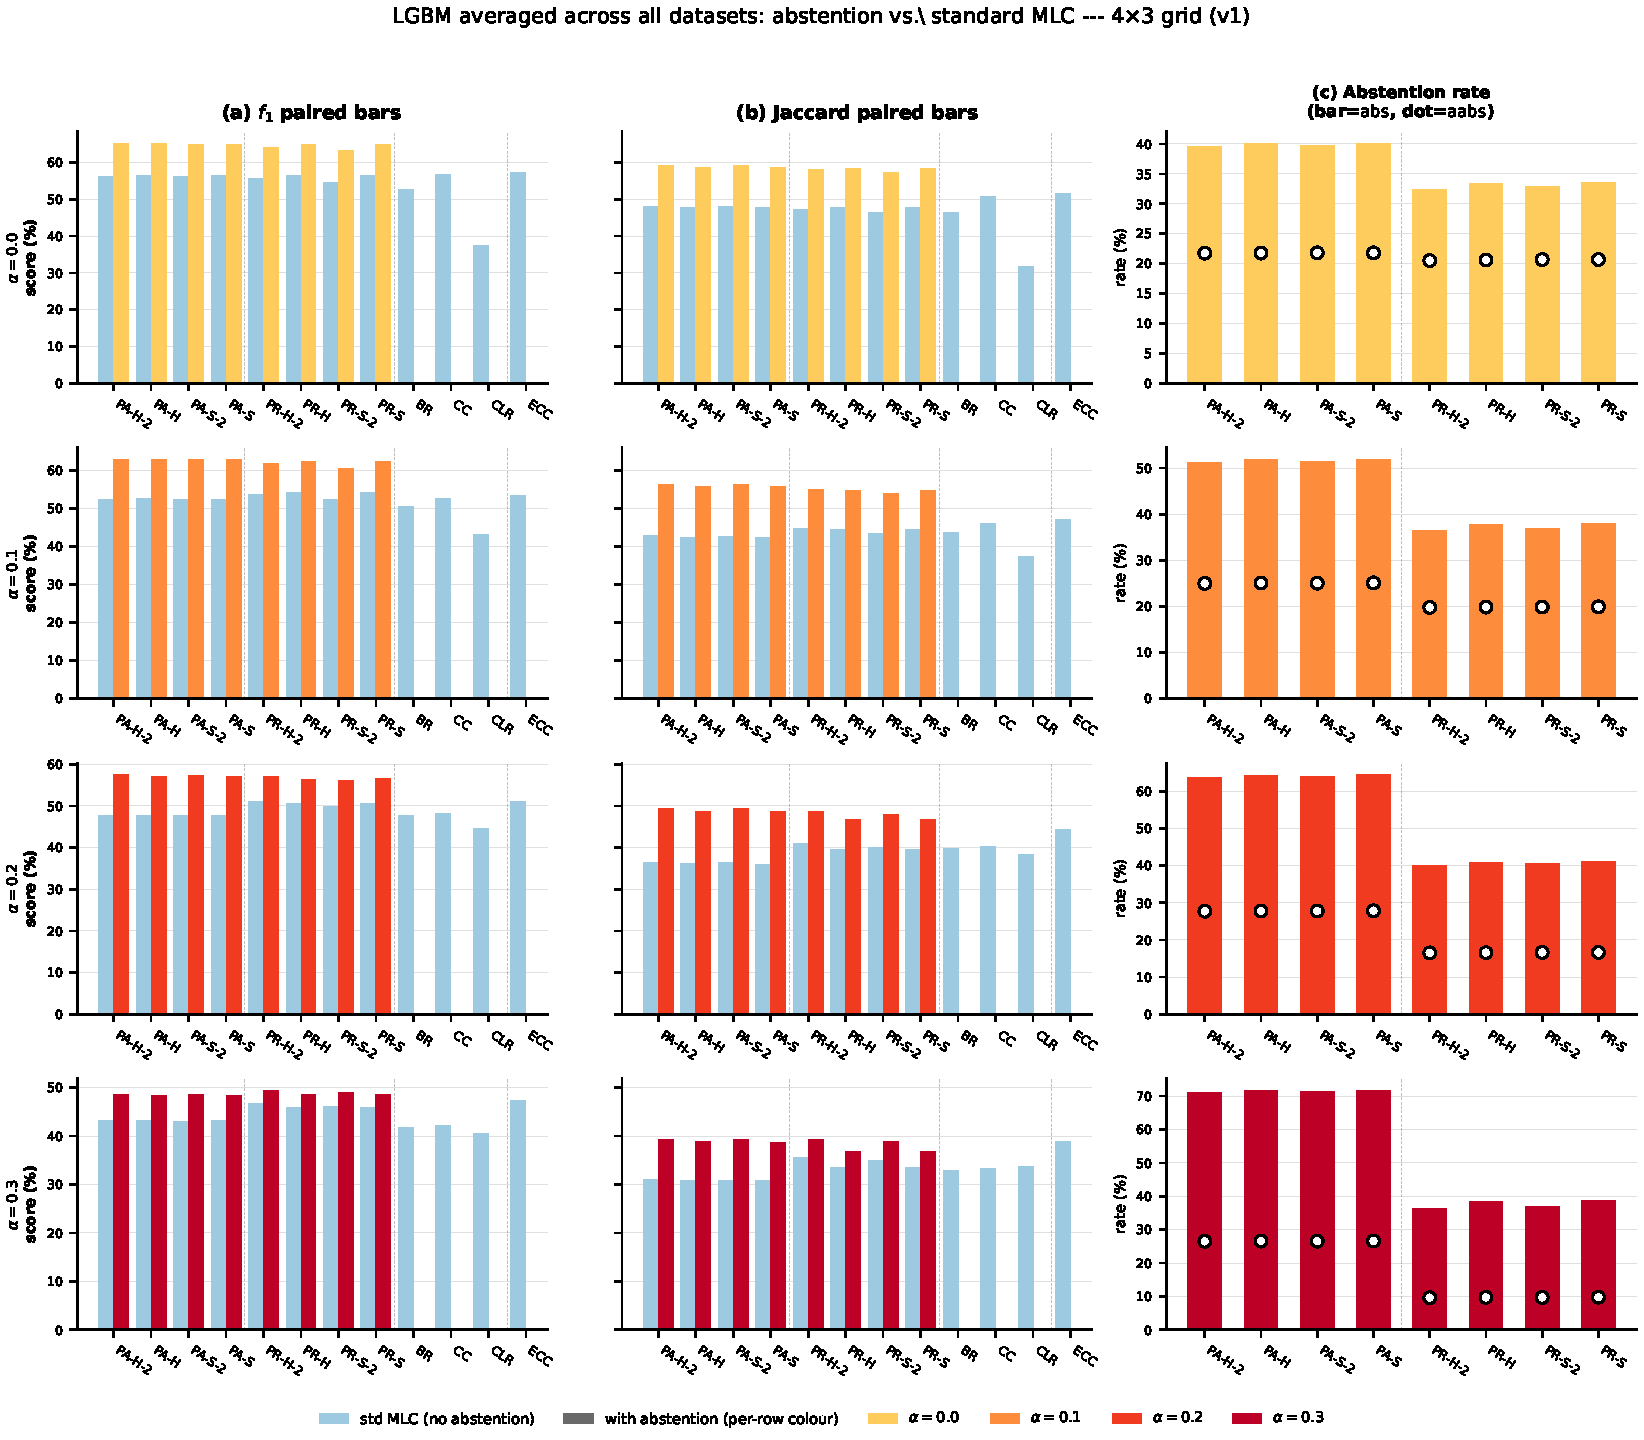
\includegraphics[width=\linewidth]{lgbm/abstain/_shared/aggregate/summary_grid.pdf}
\caption{LGBM averaged across all datasets, $4\times 3$ grid (rows $=\alpha$, cols $=$ $f_1$ / Jaccard / abstention rate) --- (version~1) all 12 methods on the $x$-axis (PA + PR + baselines BR/CC/CLR/ECC); baselines plot only the std-MLC bar since they cannot abstain. Light blue $=$ standard MLC, $\alpha$-coloured $=$ with-abstention; in (c), bar $=$ \texttt{abs} (instance-level), dot $=$ \texttt{aabs} (per-cell). Color = $\alpha\in\{0.0, 0.1, 0.2, 0.3\}$.}
\label{fig:abstain_summary_lgbm_v1}
\end{figure}

\begin{figure}[!htbp]
\centering
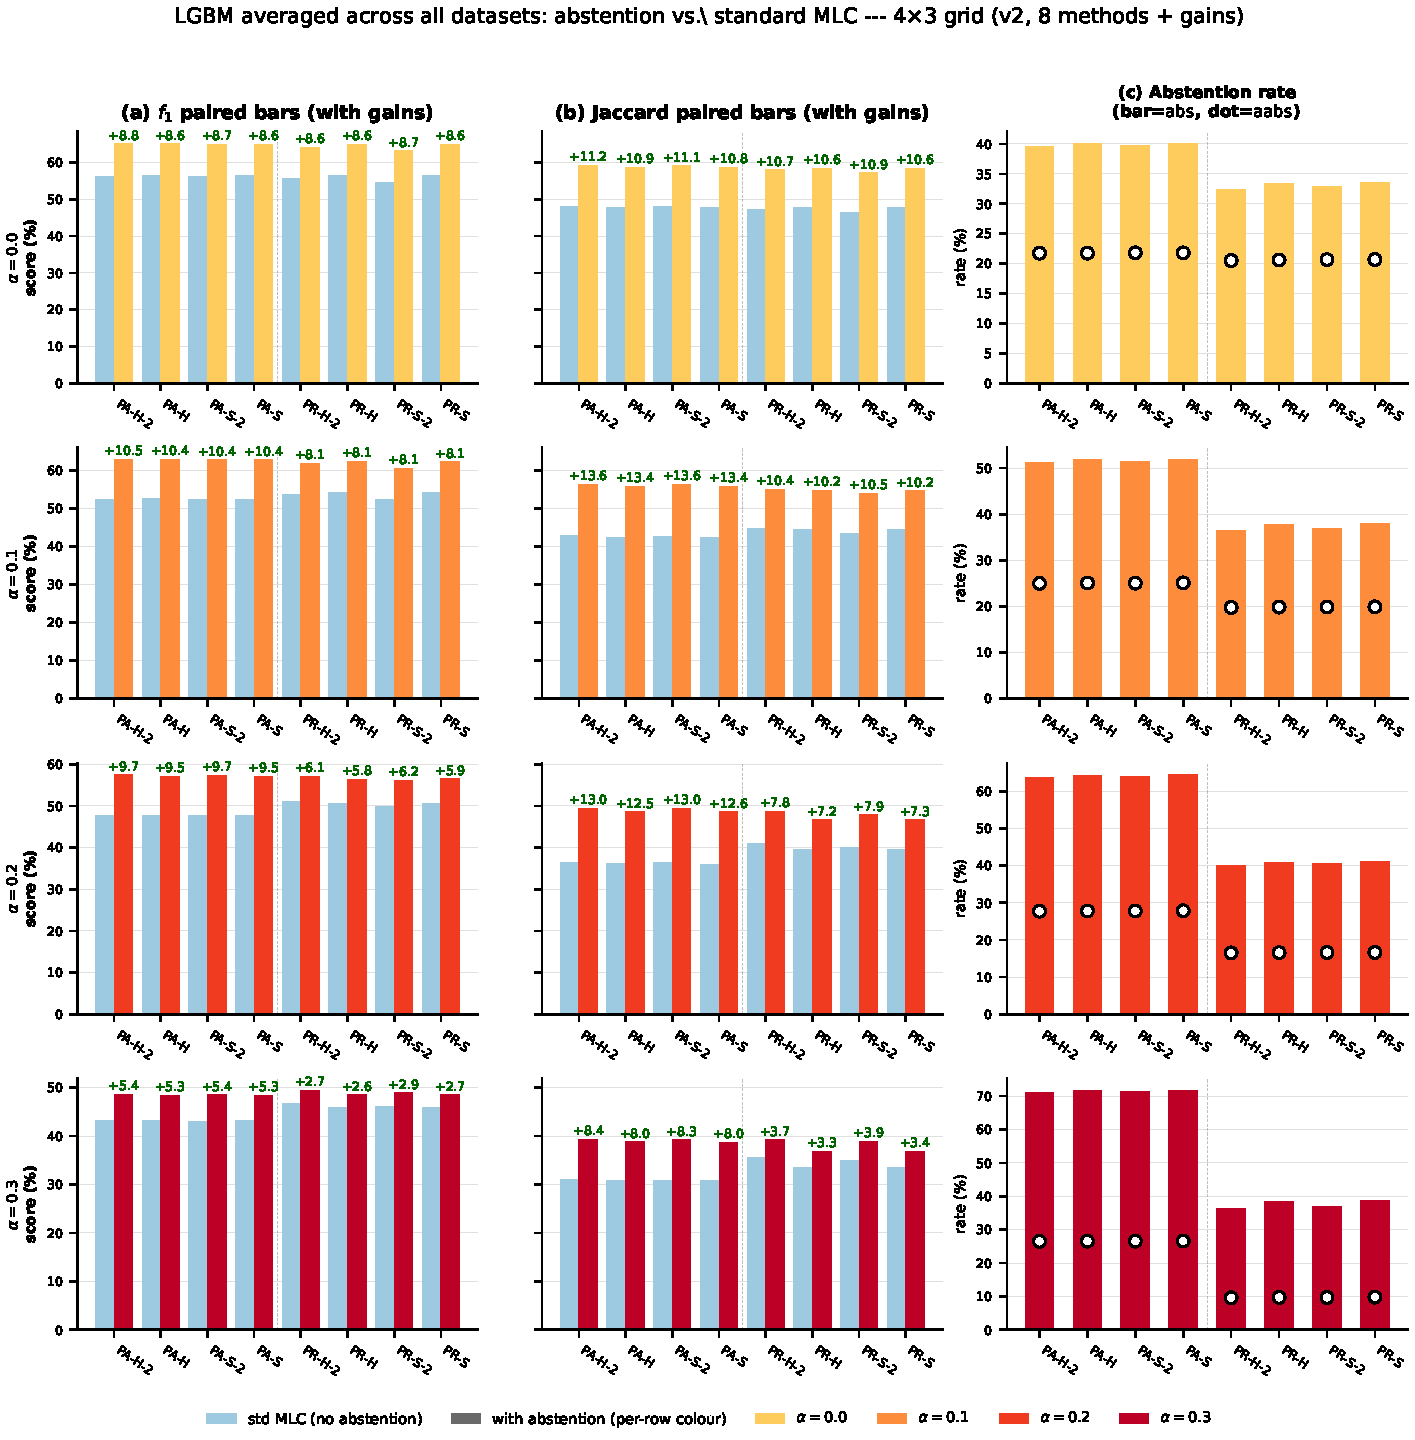
\includegraphics[width=\linewidth]{lgbm/abstain/_shared/aggregate/summary_grid_v2.pdf}
\caption{LGBM averaged across all datasets, $4\times 3$ grid (rows $=\alpha$, cols $=$ $f_1$ / Jaccard / abstention rate) --- (version~2) only the 8 PA/PR methods that can abstain; gain labels $+x.y$ printed above each with-abstention bar so the score-point benefit over the std-MLC bar at the same method is visible at a glance. Same colour / layout conventions as version~1. Color = $\alpha\in\{0.0, 0.1, 0.2, 0.3\}$.}
\label{fig:abstain_summary_lgbm_v2}
\end{figure}

\FloatBarrier
\clearpage

\clearpage

\section{Main results: RF base learner, aggregated}

\subsubsection*{RF $\bullet$ Aggregate $\bullet$ BinaryVector --- Standard MLC predictions}
\begin{table}[!htbp]
\centering
\setlength{\tabcolsep}{2pt}
\renewcommand{\arraystretch}{0.6}
\begin{tabular}{ccc}
\mpanel{rf/aggregate/bv/afrd.pdf} & \mpanel{rf/aggregate/bv/afrd_notitle.pdf} & \mpanel{rf/aggregate/bv/example_precision.pdf} \\
\mpanel{rf/aggregate/bv/example_precision_notitle.pdf} & \mpanel{rf/aggregate/bv/example_recall.pdf} & \mpanel{rf/aggregate/bv/example_recall_notitle.pdf} \\
\mpanel{rf/aggregate/bv/f1.pdf} & \mpanel{rf/aggregate/bv/f1_notitle.pdf} & \mpanel{rf/aggregate/bv/hamming_accuracy.pdf} \\
\mpanel{rf/aggregate/bv/hamming_accuracy_notitle.pdf} & \mpanel{rf/aggregate/bv/jaccard.pdf} & \mpanel{rf/aggregate/bv/jaccard_notitle.pdf} \\
\mpanel{rf/aggregate/bv/macro_f1.pdf} & \mpanel{rf/aggregate/bv/macro_f1_notitle.pdf} & \mpanel{rf/aggregate/bv/macro_precision.pdf} \\
\mpanel{rf/aggregate/bv/macro_precision_notitle.pdf} & \mpanel{rf/aggregate/bv/macro_recall.pdf} & \mpanel{rf/aggregate/bv/macro_recall_notitle.pdf} \\
\mpanel{rf/aggregate/bv/mfrd.pdf} & \mpanel{rf/aggregate/bv/mfrd_notitle.pdf} & \mpanel{rf/aggregate/bv/micro_f1.pdf} \\
\mpanel{rf/aggregate/bv/micro_f1_notitle.pdf} & \mpanel{rf/aggregate/bv/micro_precision.pdf} & \mpanel{rf/aggregate/bv/micro_precision_notitle.pdf} \\
\mpanel{rf/aggregate/bv/micro_recall.pdf} & \mpanel{rf/aggregate/bv/micro_recall_notitle.pdf} & \mpanel{rf/aggregate/bv/subset0_1.pdf} \\
\mpanel{rf/aggregate/bv/subset0_1_notitle.pdf} &  &  \\
\end{tabular}
\caption{Standard MLC predictions (BinaryVector), RF base learner, averaged across datasets. Method indices and line colors follow the encoding paragraph above.}
\label{tab:rf_agg_bv}
\end{table}

\subsubsection*{RF $\bullet$ Aggregate $\bullet$ PartialAbstention --- Partial abstention}
\begin{table}[!htbp]
\centering
\setlength{\tabcolsep}{2pt}
\renewcommand{\arraystretch}{0.6}
\begin{tabular}{ccc}
\mpanel{rf/aggregate/pa/aabs.pdf} & \mpanel{rf/aggregate/pa/aabs_notitle.pdf} & \mpanel{rf/aggregate/pa/abs.pdf} \\
\mpanel{rf/aggregate/pa/abs_notitle.pdf} & \mpanel{rf/aggregate/pa/afrd_pa.pdf} & \mpanel{rf/aggregate/pa/afrd_pa_notitle.pdf} \\
\mpanel{rf/aggregate/pa/arec.pdf} & \mpanel{rf/aggregate/pa/arec_notitle.pdf} & \mpanel{rf/aggregate/pa/example_precision_pa.pdf} \\
\mpanel{rf/aggregate/pa/example_precision_pa_notitle.pdf} & \mpanel{rf/aggregate/pa/example_recall_pa.pdf} & \mpanel{rf/aggregate/pa/example_recall_pa_notitle.pdf} \\
\mpanel{rf/aggregate/pa/f1_pa.pdf} & \mpanel{rf/aggregate/pa/f1_pa_notitle.pdf} & \mpanel{rf/aggregate/pa/hamming_accuracy_pa.pdf} \\
\mpanel{rf/aggregate/pa/hamming_accuracy_pa_notitle.pdf} & \mpanel{rf/aggregate/pa/jaccard_pa.pdf} & \mpanel{rf/aggregate/pa/jaccard_pa_notitle.pdf} \\
\mpanel{rf/aggregate/pa/macro_f1_pa.pdf} & \mpanel{rf/aggregate/pa/macro_f1_pa_notitle.pdf} & \mpanel{rf/aggregate/pa/macro_precision_pa.pdf} \\
\mpanel{rf/aggregate/pa/macro_precision_pa_notitle.pdf} & \mpanel{rf/aggregate/pa/macro_recall_pa.pdf} & \mpanel{rf/aggregate/pa/macro_recall_pa_notitle.pdf} \\
\mpanel{rf/aggregate/pa/mfrd_pa.pdf} & \mpanel{rf/aggregate/pa/mfrd_pa_notitle.pdf} & \mpanel{rf/aggregate/pa/micro_f1_pa.pdf} \\
\mpanel{rf/aggregate/pa/micro_f1_pa_notitle.pdf} & \mpanel{rf/aggregate/pa/micro_precision_pa.pdf} & \mpanel{rf/aggregate/pa/micro_precision_pa_notitle.pdf} \\
\mpanel{rf/aggregate/pa/micro_recall_pa.pdf} & \mpanel{rf/aggregate/pa/micro_recall_pa_notitle.pdf} & \mpanel{rf/aggregate/pa/rec.pdf} \\
\mpanel{rf/aggregate/pa/rec_notitle.pdf} & \mpanel{rf/aggregate/pa/subset0_1_pa.pdf} & \mpanel{rf/aggregate/pa/subset0_1_pa_notitle.pdf} \\
\end{tabular}
\caption{Partial abstention (PartialAbstention), RF base learner, averaged across datasets. Method indices and line colors follow the encoding paragraph above.}
\label{tab:rf_agg_pa}
\end{table}

\subsubsection*{RF $\bullet$ Aggregate $\bullet$ ScoreVector --- Score-vector ranking metrics (AUROC, AUPRC, etc.)}
\begin{table}[!htbp]
\centering
\setlength{\tabcolsep}{2pt}
\renewcommand{\arraystretch}{0.6}
\begin{tabular}{ccc}
\mpanel{rf/aggregate/sv/auc_macro.pdf} & \mpanel{rf/aggregate/sv/auc_macro_notitle.pdf} & \mpanel{rf/aggregate/sv/auc_micro.pdf} \\
\mpanel{rf/aggregate/sv/auc_micro_notitle.pdf} & \mpanel{rf/aggregate/sv/auprc_macro.pdf} & \mpanel{rf/aggregate/sv/auprc_macro_notitle.pdf} \\
\mpanel{rf/aggregate/sv/auprc_micro.pdf} & \mpanel{rf/aggregate/sv/auprc_micro_notitle.pdf} & \mpanel{rf/aggregate/sv/coverage.pdf} \\
\mpanel{rf/aggregate/sv/coverage_notitle.pdf} & \mpanel{rf/aggregate/sv/lr_ap.pdf} & \mpanel{rf/aggregate/sv/lr_ap_notitle.pdf} \\
\mpanel{rf/aggregate/sv/one_error.pdf} & \mpanel{rf/aggregate/sv/one_error_notitle.pdf} & \mpanel{rf/aggregate/sv/ranking_loss.pdf} \\
\mpanel{rf/aggregate/sv/ranking_loss_notitle.pdf} &  &  \\
\end{tabular}
\caption{Score-vector ranking metrics (AUROC, AUPRC, etc.) (ScoreVector), RF base learner, averaged across datasets. Method indices and line colors follow the encoding paragraph above.}
\label{tab:rf_agg_sv}
\end{table}

\clearpage

\section{Abstention vs standard MLC}\label{sec:abstain_vs_mlc}
\paragraph{Why this section exists.} The paper's central claim is that an order-based predictor can \emph{abstain} on labels it is unsure about and, on the labels it does predict, achieve higher quality than a standard MLC method that is forced to predict every label. The two chart families below make that claim visible.

\paragraph{Terminology.} `\emph{Standard MLC}' (a.k.a.\ \texttt{BinaryVector} / BV) means each method outputs a 0/1 prediction for every one of the $K$ labels. `\emph{With abstention}' (a.k.a.\ \texttt{PartialAbstention} / PA) means an order-based predictor may return $\bot$ (abstain) on some labels; the PA quality metrics (\texttt{f1\_pa}, \texttt{jaccard\_pa}, \ldots) are computed only over the non-abstained labels. Only the 8 PA/PR methods (indices 1--8) can abstain; BR/CC/CLR/ECC cannot.

\paragraph{Reading the coverage-risk chart.} Each point is one (PA/PR method, noise level $\alpha$) pair. The x-axis is the abstention rate (fraction of labels the method skipped); the y-axis is the quality metric on the labels that \emph{were} predicted (higher is better). Marker shape encodes method, colour encodes noise level. The dashed grey line is the best standard-MLC baseline (BR / CC / CLR / ECC) on the BV quality metric --- it is the bar that ``no abstention'' has to clear. \textbf{Any point above the dashed line is direct evidence that abstaining improved quality beyond what any standard MLC method achieves.} Points further right traded coverage for that gain.

\paragraph{Reading the paired-bars chart.} Same data, different view. The four sub-panels correspond to the four noise levels. Inside each sub-panel: 12 method positions, two bars per position --- blue is the standard-MLC quality (\texttt{f1}, no abstention), warm-colour is the with-abstention quality on retained labels. Only the 8 PA/PR methods (1--8) have a warm bar; the standard MLC baselines (9--12) only have a blue bar by construction. The green ``$+x.y$'' label above each warm bar is the gain in score-points over that method's own BV bar.

\subsection{RF, metric \texttt{f1\_pa} --- aggregate}

\begin{figure}[!htbp]
\centering
\mpanel{rf/abstain/_shared/aggregate/abstention_rate.pdf}\hfill
\mpanel{rf/abstain/f1_pa/aggregate/paired_bars.pdf}
\caption{RF (f1\_pa) averaged across all datasets: abstention rates (left) and standard-MLC-vs-abstention paired bars (right), across $\alpha\in\{0.0,0.1,0.2,0.3\}$. Left: bar = \texttt{abs} (\% of instances with at least one abstained label, instance-level); dot = \texttt{aabs} (\% of labels skipped, per-cell label-level). These rates are independent of the quality metric. Right: blue = standard MLC quality (no abstention) on the matched BV metric; coloured = with-abstention quality on retained labels.}
\label{fig:abstain_rf_f1_pa_agg_rates_quality}
\end{figure}

\begin{figure}[!htbp]
\centering
\mpanel{rf/abstain/f1_pa/aggregate/coverage_risk.pdf}
\caption{RF (f1\_pa) averaged across all datasets: coverage-risk scatter. Each point is one (method, noise) pair; x = abstention rate, y = quality on retained labels. Points above the dashed line beat the best standard-MLC baseline.}
\label{fig:abstain_rf_f1_pa_agg_coverage_risk}
\end{figure}

\begin{figure}[!htbp]
\centering
\mpanel{rf/abstain/f1_pa/aggregate/coverage_risk_pareto.pdf}\hfill
\mpanel{rf/abstain/f1_pa/aggregate/gain_heatmap.pdf}
\caption{RF (f1\_pa) averaged across all datasets: Pareto frontier of (abstention, retained quality) with the win-region shaded green (left); per-method per-noise gain $(\text{f1\_pa}-f_1)$ heatmap (right).}
\label{fig:abstain_rf_f1_pa_agg_gain}
\end{figure}

\begin{figure}[!htbp]
\centering
\mpanel{rf/abstain/f1_pa/aggregate/efficiency_quality.pdf}\hfill
\mpanel{rf/abstain/f1_pa/aggregate/effective_f1.pdf}
\caption{RF (f1\_pa) averaged across all datasets --- robustness view. Left: efficiency-quality scatter (x = coverage $= 1-\text{abs}$); upper-right is robust (predicts many labels and keeps quality high). Right: effective f1\_pa $= (1-\text{abs}) \cdot f1\_pa$, i.e.\ retained quality penalised by skipped coverage. A method whose effective curve stays above the dashed standard-MLC baseline at every $\alpha$ is robust to noise, not just selectively abstaining on hard labels.}
\label{fig:abstain_rf_f1_pa_agg_robust}
\end{figure}

\FloatBarrier

\subsection{RF, metric \texttt{f1\_pa} --- per dataset}

\begin{figure}[!htbp]
\centering
\mpanel{rf/abstain/_shared/per_dataset/GpositivePseAAC/abstention_rate.pdf}\hfill
\mpanel{rf/abstain/f1_pa/per_dataset/GpositivePseAAC/paired_bars.pdf}
\caption{RF (f1\_pa) on \texttt{GpositivePseAAC}: abstention rates (left) and standard-MLC-vs-abstention paired bars (right), across $\alpha\in\{0.0,0.1,0.2,0.3\}$. Left: bar = \texttt{abs} (\% of instances with at least one abstained label, instance-level); dot = \texttt{aabs} (\% of labels skipped, per-cell label-level). These rates are independent of the quality metric. Right: blue = standard MLC quality (no abstention) on the matched BV metric; coloured = with-abstention quality on retained labels.}
\label{fig:abstain_rf_f1_pa_GpositivePseAAC_rates_quality}
\end{figure}

\begin{figure}[!htbp]
\centering
\mpanel{rf/abstain/f1_pa/per_dataset/GpositivePseAAC/coverage_risk.pdf}
\caption{RF (f1\_pa) on \texttt{GpositivePseAAC}: coverage-risk scatter. Each point is one (method, noise) pair; x = abstention rate, y = quality on retained labels. Points above the dashed line beat the best standard-MLC baseline.}
\label{fig:abstain_rf_f1_pa_GpositivePseAAC_coverage_risk}
\end{figure}

\begin{figure}[!htbp]
\centering
\mpanel{rf/abstain/f1_pa/per_dataset/GpositivePseAAC/coverage_risk_pareto.pdf}\hfill
\mpanel{rf/abstain/f1_pa/per_dataset/GpositivePseAAC/gain_heatmap.pdf}
\caption{RF (f1\_pa) on \texttt{GpositivePseAAC}: Pareto frontier of (abstention, retained quality) with the win-region shaded green (left); per-method per-noise gain $(\text{f1\_pa}-f_1)$ heatmap (right).}
\label{fig:abstain_rf_f1_pa_GpositivePseAAC_gain}
\end{figure}

\begin{figure}[!htbp]
\centering
\mpanel{rf/abstain/f1_pa/per_dataset/GpositivePseAAC/efficiency_quality.pdf}\hfill
\mpanel{rf/abstain/f1_pa/per_dataset/GpositivePseAAC/effective_f1.pdf}
\caption{RF (f1\_pa) on \texttt{GpositivePseAAC} --- robustness view. Left: efficiency-quality scatter (x = coverage $= 1-\text{abs}$); upper-right is robust (predicts many labels and keeps quality high). Right: effective f1\_pa $= (1-\text{abs}) \cdot f1\_pa$, i.e.\ retained quality penalised by skipped coverage. A method whose effective curve stays above the dashed standard-MLC baseline at every $\alpha$ is robust to noise, not just selectively abstaining on hard labels.}
\label{fig:abstain_rf_f1_pa_GpositivePseAAC_robust}
\end{figure}

\FloatBarrier

\begin{figure}[!htbp]
\centering
\mpanel{rf/abstain/_shared/per_dataset/emotions/abstention_rate.pdf}\hfill
\mpanel{rf/abstain/f1_pa/per_dataset/emotions/paired_bars.pdf}
\caption{RF (f1\_pa) on \texttt{emotions}: abstention rates (left) and standard-MLC-vs-abstention paired bars (right), across $\alpha\in\{0.0,0.1,0.2,0.3\}$. Left: bar = \texttt{abs} (\% of instances with at least one abstained label, instance-level); dot = \texttt{aabs} (\% of labels skipped, per-cell label-level). These rates are independent of the quality metric. Right: blue = standard MLC quality (no abstention) on the matched BV metric; coloured = with-abstention quality on retained labels.}
\label{fig:abstain_rf_f1_pa_emotions_rates_quality}
\end{figure}

\begin{figure}[!htbp]
\centering
\mpanel{rf/abstain/f1_pa/per_dataset/emotions/coverage_risk.pdf}
\caption{RF (f1\_pa) on \texttt{emotions}: coverage-risk scatter. Each point is one (method, noise) pair; x = abstention rate, y = quality on retained labels. Points above the dashed line beat the best standard-MLC baseline.}
\label{fig:abstain_rf_f1_pa_emotions_coverage_risk}
\end{figure}

\begin{figure}[!htbp]
\centering
\mpanel{rf/abstain/f1_pa/per_dataset/emotions/coverage_risk_pareto.pdf}\hfill
\mpanel{rf/abstain/f1_pa/per_dataset/emotions/gain_heatmap.pdf}
\caption{RF (f1\_pa) on \texttt{emotions}: Pareto frontier of (abstention, retained quality) with the win-region shaded green (left); per-method per-noise gain $(\text{f1\_pa}-f_1)$ heatmap (right).}
\label{fig:abstain_rf_f1_pa_emotions_gain}
\end{figure}

\begin{figure}[!htbp]
\centering
\mpanel{rf/abstain/f1_pa/per_dataset/emotions/efficiency_quality.pdf}\hfill
\mpanel{rf/abstain/f1_pa/per_dataset/emotions/effective_f1.pdf}
\caption{RF (f1\_pa) on \texttt{emotions} --- robustness view. Left: efficiency-quality scatter (x = coverage $= 1-\text{abs}$); upper-right is robust (predicts many labels and keeps quality high). Right: effective f1\_pa $= (1-\text{abs}) \cdot f1\_pa$, i.e.\ retained quality penalised by skipped coverage. A method whose effective curve stays above the dashed standard-MLC baseline at every $\alpha$ is robust to noise, not just selectively abstaining on hard labels.}
\label{fig:abstain_rf_f1_pa_emotions_robust}
\end{figure}

\FloatBarrier

\begin{figure}[!htbp]
\centering
\mpanel{rf/abstain/_shared/per_dataset/scene/abstention_rate.pdf}\hfill
\mpanel{rf/abstain/f1_pa/per_dataset/scene/paired_bars.pdf}
\caption{RF (f1\_pa) on \texttt{scene}: abstention rates (left) and standard-MLC-vs-abstention paired bars (right), across $\alpha\in\{0.0,0.1,0.2,0.3\}$. Left: bar = \texttt{abs} (\% of instances with at least one abstained label, instance-level); dot = \texttt{aabs} (\% of labels skipped, per-cell label-level). These rates are independent of the quality metric. Right: blue = standard MLC quality (no abstention) on the matched BV metric; coloured = with-abstention quality on retained labels.}
\label{fig:abstain_rf_f1_pa_scene_rates_quality}
\end{figure}

\begin{figure}[!htbp]
\centering
\mpanel{rf/abstain/f1_pa/per_dataset/scene/coverage_risk.pdf}
\caption{RF (f1\_pa) on \texttt{scene}: coverage-risk scatter. Each point is one (method, noise) pair; x = abstention rate, y = quality on retained labels. Points above the dashed line beat the best standard-MLC baseline.}
\label{fig:abstain_rf_f1_pa_scene_coverage_risk}
\end{figure}

\begin{figure}[!htbp]
\centering
\mpanel{rf/abstain/f1_pa/per_dataset/scene/coverage_risk_pareto.pdf}\hfill
\mpanel{rf/abstain/f1_pa/per_dataset/scene/gain_heatmap.pdf}
\caption{RF (f1\_pa) on \texttt{scene}: Pareto frontier of (abstention, retained quality) with the win-region shaded green (left); per-method per-noise gain $(\text{f1\_pa}-f_1)$ heatmap (right).}
\label{fig:abstain_rf_f1_pa_scene_gain}
\end{figure}

\begin{figure}[!htbp]
\centering
\mpanel{rf/abstain/f1_pa/per_dataset/scene/efficiency_quality.pdf}\hfill
\mpanel{rf/abstain/f1_pa/per_dataset/scene/effective_f1.pdf}
\caption{RF (f1\_pa) on \texttt{scene} --- robustness view. Left: efficiency-quality scatter (x = coverage $= 1-\text{abs}$); upper-right is robust (predicts many labels and keeps quality high). Right: effective f1\_pa $= (1-\text{abs}) \cdot f1\_pa$, i.e.\ retained quality penalised by skipped coverage. A method whose effective curve stays above the dashed standard-MLC baseline at every $\alpha$ is robust to noise, not just selectively abstaining on hard labels.}
\label{fig:abstain_rf_f1_pa_scene_robust}
\end{figure}

\FloatBarrier

\begin{figure}[!htbp]
\centering
\mpanel{rf/abstain/_shared/per_dataset/PlantPseAAC/abstention_rate.pdf}\hfill
\mpanel{rf/abstain/f1_pa/per_dataset/PlantPseAAC/paired_bars.pdf}
\caption{RF (f1\_pa) on \texttt{PlantPseAAC}: abstention rates (left) and standard-MLC-vs-abstention paired bars (right), across $\alpha\in\{0.0,0.1,0.2,0.3\}$. Left: bar = \texttt{abs} (\% of instances with at least one abstained label, instance-level); dot = \texttt{aabs} (\% of labels skipped, per-cell label-level). These rates are independent of the quality metric. Right: blue = standard MLC quality (no abstention) on the matched BV metric; coloured = with-abstention quality on retained labels.}
\label{fig:abstain_rf_f1_pa_PlantPseAAC_rates_quality}
\end{figure}

\begin{figure}[!htbp]
\centering
\mpanel{rf/abstain/f1_pa/per_dataset/PlantPseAAC/coverage_risk.pdf}
\caption{RF (f1\_pa) on \texttt{PlantPseAAC}: coverage-risk scatter. Each point is one (method, noise) pair; x = abstention rate, y = quality on retained labels. Points above the dashed line beat the best standard-MLC baseline.}
\label{fig:abstain_rf_f1_pa_PlantPseAAC_coverage_risk}
\end{figure}

\begin{figure}[!htbp]
\centering
\mpanel{rf/abstain/f1_pa/per_dataset/PlantPseAAC/coverage_risk_pareto.pdf}\hfill
\mpanel{rf/abstain/f1_pa/per_dataset/PlantPseAAC/gain_heatmap.pdf}
\caption{RF (f1\_pa) on \texttt{PlantPseAAC}: Pareto frontier of (abstention, retained quality) with the win-region shaded green (left); per-method per-noise gain $(\text{f1\_pa}-f_1)$ heatmap (right).}
\label{fig:abstain_rf_f1_pa_PlantPseAAC_gain}
\end{figure}

\begin{figure}[!htbp]
\centering
\mpanel{rf/abstain/f1_pa/per_dataset/PlantPseAAC/efficiency_quality.pdf}\hfill
\mpanel{rf/abstain/f1_pa/per_dataset/PlantPseAAC/effective_f1.pdf}
\caption{RF (f1\_pa) on \texttt{PlantPseAAC} --- robustness view. Left: efficiency-quality scatter (x = coverage $= 1-\text{abs}$); upper-right is robust (predicts many labels and keeps quality high). Right: effective f1\_pa $= (1-\text{abs}) \cdot f1\_pa$, i.e.\ retained quality penalised by skipped coverage. A method whose effective curve stays above the dashed standard-MLC baseline at every $\alpha$ is robust to noise, not just selectively abstaining on hard labels.}
\label{fig:abstain_rf_f1_pa_PlantPseAAC_robust}
\end{figure}

\FloatBarrier

\begin{figure}[!htbp]
\centering
\mpanel{rf/abstain/_shared/per_dataset/HumanPseAAC/abstention_rate.pdf}\hfill
\mpanel{rf/abstain/f1_pa/per_dataset/HumanPseAAC/paired_bars.pdf}
\caption{RF (f1\_pa) on \texttt{HumanPseAAC}: abstention rates (left) and standard-MLC-vs-abstention paired bars (right), across $\alpha\in\{0.0,0.1,0.2,0.3\}$. Left: bar = \texttt{abs} (\% of instances with at least one abstained label, instance-level); dot = \texttt{aabs} (\% of labels skipped, per-cell label-level). These rates are independent of the quality metric. Right: blue = standard MLC quality (no abstention) on the matched BV metric; coloured = with-abstention quality on retained labels.}
\label{fig:abstain_rf_f1_pa_HumanPseAAC_rates_quality}
\end{figure}

\begin{figure}[!htbp]
\centering
\mpanel{rf/abstain/f1_pa/per_dataset/HumanPseAAC/coverage_risk.pdf}
\caption{RF (f1\_pa) on \texttt{HumanPseAAC}: coverage-risk scatter. Each point is one (method, noise) pair; x = abstention rate, y = quality on retained labels. Points above the dashed line beat the best standard-MLC baseline.}
\label{fig:abstain_rf_f1_pa_HumanPseAAC_coverage_risk}
\end{figure}

\begin{figure}[!htbp]
\centering
\mpanel{rf/abstain/f1_pa/per_dataset/HumanPseAAC/coverage_risk_pareto.pdf}\hfill
\mpanel{rf/abstain/f1_pa/per_dataset/HumanPseAAC/gain_heatmap.pdf}
\caption{RF (f1\_pa) on \texttt{HumanPseAAC}: Pareto frontier of (abstention, retained quality) with the win-region shaded green (left); per-method per-noise gain $(\text{f1\_pa}-f_1)$ heatmap (right).}
\label{fig:abstain_rf_f1_pa_HumanPseAAC_gain}
\end{figure}

\begin{figure}[!htbp]
\centering
\mpanel{rf/abstain/f1_pa/per_dataset/HumanPseAAC/efficiency_quality.pdf}\hfill
\mpanel{rf/abstain/f1_pa/per_dataset/HumanPseAAC/effective_f1.pdf}
\caption{RF (f1\_pa) on \texttt{HumanPseAAC} --- robustness view. Left: efficiency-quality scatter (x = coverage $= 1-\text{abs}$); upper-right is robust (predicts many labels and keeps quality high). Right: effective f1\_pa $= (1-\text{abs}) \cdot f1\_pa$, i.e.\ retained quality penalised by skipped coverage. A method whose effective curve stays above the dashed standard-MLC baseline at every $\alpha$ is robust to noise, not just selectively abstaining on hard labels.}
\label{fig:abstain_rf_f1_pa_HumanPseAAC_robust}
\end{figure}

\FloatBarrier

\begin{figure}[!htbp]
\centering
\mpanel{rf/abstain/_shared/per_dataset/Yeast/abstention_rate.pdf}\hfill
\mpanel{rf/abstain/f1_pa/per_dataset/Yeast/paired_bars.pdf}
\caption{RF (f1\_pa) on \texttt{Yeast}: abstention rates (left) and standard-MLC-vs-abstention paired bars (right), across $\alpha\in\{0.0,0.1,0.2,0.3\}$. Left: bar = \texttt{abs} (\% of instances with at least one abstained label, instance-level); dot = \texttt{aabs} (\% of labels skipped, per-cell label-level). These rates are independent of the quality metric. Right: blue = standard MLC quality (no abstention) on the matched BV metric; coloured = with-abstention quality on retained labels.}
\label{fig:abstain_rf_f1_pa_Yeast_rates_quality}
\end{figure}

\begin{figure}[!htbp]
\centering
\mpanel{rf/abstain/f1_pa/per_dataset/Yeast/coverage_risk.pdf}
\caption{RF (f1\_pa) on \texttt{Yeast}: coverage-risk scatter. Each point is one (method, noise) pair; x = abstention rate, y = quality on retained labels. Points above the dashed line beat the best standard-MLC baseline.}
\label{fig:abstain_rf_f1_pa_Yeast_coverage_risk}
\end{figure}

\begin{figure}[!htbp]
\centering
\mpanel{rf/abstain/f1_pa/per_dataset/Yeast/coverage_risk_pareto.pdf}\hfill
\mpanel{rf/abstain/f1_pa/per_dataset/Yeast/gain_heatmap.pdf}
\caption{RF (f1\_pa) on \texttt{Yeast}: Pareto frontier of (abstention, retained quality) with the win-region shaded green (left); per-method per-noise gain $(\text{f1\_pa}-f_1)$ heatmap (right).}
\label{fig:abstain_rf_f1_pa_Yeast_gain}
\end{figure}

\begin{figure}[!htbp]
\centering
\mpanel{rf/abstain/f1_pa/per_dataset/Yeast/efficiency_quality.pdf}\hfill
\mpanel{rf/abstain/f1_pa/per_dataset/Yeast/effective_f1.pdf}
\caption{RF (f1\_pa) on \texttt{Yeast} --- robustness view. Left: efficiency-quality scatter (x = coverage $= 1-\text{abs}$); upper-right is robust (predicts many labels and keeps quality high). Right: effective f1\_pa $= (1-\text{abs}) \cdot f1\_pa$, i.e.\ retained quality penalised by skipped coverage. A method whose effective curve stays above the dashed standard-MLC baseline at every $\alpha$ is robust to noise, not just selectively abstaining on hard labels.}
\label{fig:abstain_rf_f1_pa_Yeast_robust}
\end{figure}

\FloatBarrier

\begin{figure}[!htbp]
\centering
\mpanel{rf/abstain/_shared/per_dataset/CHD_49/abstention_rate.pdf}\hfill
\mpanel{rf/abstain/f1_pa/per_dataset/CHD_49/paired_bars.pdf}
\caption{RF (f1\_pa) on \texttt{CHD\_49}: abstention rates (left) and standard-MLC-vs-abstention paired bars (right), across $\alpha\in\{0.0,0.1,0.2,0.3\}$. Left: bar = \texttt{abs} (\% of instances with at least one abstained label, instance-level); dot = \texttt{aabs} (\% of labels skipped, per-cell label-level). These rates are independent of the quality metric. Right: blue = standard MLC quality (no abstention) on the matched BV metric; coloured = with-abstention quality on retained labels.}
\label{fig:abstain_rf_f1_pa_CHD_49_rates_quality}
\end{figure}

\begin{figure}[!htbp]
\centering
\mpanel{rf/abstain/f1_pa/per_dataset/CHD_49/coverage_risk.pdf}
\caption{RF (f1\_pa) on \texttt{CHD\_49}: coverage-risk scatter. Each point is one (method, noise) pair; x = abstention rate, y = quality on retained labels. Points above the dashed line beat the best standard-MLC baseline.}
\label{fig:abstain_rf_f1_pa_CHD_49_coverage_risk}
\end{figure}

\begin{figure}[!htbp]
\centering
\mpanel{rf/abstain/f1_pa/per_dataset/CHD_49/coverage_risk_pareto.pdf}\hfill
\mpanel{rf/abstain/f1_pa/per_dataset/CHD_49/gain_heatmap.pdf}
\caption{RF (f1\_pa) on \texttt{CHD\_49}: Pareto frontier of (abstention, retained quality) with the win-region shaded green (left); per-method per-noise gain $(\text{f1\_pa}-f_1)$ heatmap (right).}
\label{fig:abstain_rf_f1_pa_CHD_49_gain}
\end{figure}

\begin{figure}[!htbp]
\centering
\mpanel{rf/abstain/f1_pa/per_dataset/CHD_49/efficiency_quality.pdf}\hfill
\mpanel{rf/abstain/f1_pa/per_dataset/CHD_49/effective_f1.pdf}
\caption{RF (f1\_pa) on \texttt{CHD\_49} --- robustness view. Left: efficiency-quality scatter (x = coverage $= 1-\text{abs}$); upper-right is robust (predicts many labels and keeps quality high). Right: effective f1\_pa $= (1-\text{abs}) \cdot f1\_pa$, i.e.\ retained quality penalised by skipped coverage. A method whose effective curve stays above the dashed standard-MLC baseline at every $\alpha$ is robust to noise, not just selectively abstaining on hard labels.}
\label{fig:abstain_rf_f1_pa_CHD_49_robust}
\end{figure}

\FloatBarrier

\begin{figure}[!htbp]
\centering
\mpanel{rf/abstain/_shared/per_dataset/Water-quality/abstention_rate.pdf}\hfill
\mpanel{rf/abstain/f1_pa/per_dataset/Water-quality/paired_bars.pdf}
\caption{RF (f1\_pa) on \texttt{Water-quality}: abstention rates (left) and standard-MLC-vs-abstention paired bars (right), across $\alpha\in\{0.0,0.1,0.2,0.3\}$. Left: bar = \texttt{abs} (\% of instances with at least one abstained label, instance-level); dot = \texttt{aabs} (\% of labels skipped, per-cell label-level). These rates are independent of the quality metric. Right: blue = standard MLC quality (no abstention) on the matched BV metric; coloured = with-abstention quality on retained labels.}
\label{fig:abstain_rf_f1_pa_Water-quality_rates_quality}
\end{figure}

\begin{figure}[!htbp]
\centering
\mpanel{rf/abstain/f1_pa/per_dataset/Water-quality/coverage_risk.pdf}
\caption{RF (f1\_pa) on \texttt{Water-quality}: coverage-risk scatter. Each point is one (method, noise) pair; x = abstention rate, y = quality on retained labels. Points above the dashed line beat the best standard-MLC baseline.}
\label{fig:abstain_rf_f1_pa_Water-quality_coverage_risk}
\end{figure}

\begin{figure}[!htbp]
\centering
\mpanel{rf/abstain/f1_pa/per_dataset/Water-quality/coverage_risk_pareto.pdf}\hfill
\mpanel{rf/abstain/f1_pa/per_dataset/Water-quality/gain_heatmap.pdf}
\caption{RF (f1\_pa) on \texttt{Water-quality}: Pareto frontier of (abstention, retained quality) with the win-region shaded green (left); per-method per-noise gain $(\text{f1\_pa}-f_1)$ heatmap (right).}
\label{fig:abstain_rf_f1_pa_Water-quality_gain}
\end{figure}

\begin{figure}[!htbp]
\centering
\mpanel{rf/abstain/f1_pa/per_dataset/Water-quality/efficiency_quality.pdf}\hfill
\mpanel{rf/abstain/f1_pa/per_dataset/Water-quality/effective_f1.pdf}
\caption{RF (f1\_pa) on \texttt{Water-quality} --- robustness view. Left: efficiency-quality scatter (x = coverage $= 1-\text{abs}$); upper-right is robust (predicts many labels and keeps quality high). Right: effective f1\_pa $= (1-\text{abs}) \cdot f1\_pa$, i.e.\ retained quality penalised by skipped coverage. A method whose effective curve stays above the dashed standard-MLC baseline at every $\alpha$ is robust to noise, not just selectively abstaining on hard labels.}
\label{fig:abstain_rf_f1_pa_Water-quality_robust}
\end{figure}

\FloatBarrier

\begin{figure}[!htbp]
\centering
\mpanel{rf/abstain/_shared/per_dataset/enron/abstention_rate.pdf}\hfill
\mpanel{rf/abstain/f1_pa/per_dataset/enron/paired_bars.pdf}
\caption{RF (f1\_pa) on \texttt{enron}: abstention rates (left) and standard-MLC-vs-abstention paired bars (right), across $\alpha\in\{0.0,0.1,0.2,0.3\}$. Left: bar = \texttt{abs} (\% of instances with at least one abstained label, instance-level); dot = \texttt{aabs} (\% of labels skipped, per-cell label-level). These rates are independent of the quality metric. Right: blue = standard MLC quality (no abstention) on the matched BV metric; coloured = with-abstention quality on retained labels.}
\label{fig:abstain_rf_f1_pa_enron_rates_quality}
\end{figure}

\begin{figure}[!htbp]
\centering
\mpanel{rf/abstain/f1_pa/per_dataset/enron/coverage_risk.pdf}
\caption{RF (f1\_pa) on \texttt{enron}: coverage-risk scatter. Each point is one (method, noise) pair; x = abstention rate, y = quality on retained labels. Points above the dashed line beat the best standard-MLC baseline.}
\label{fig:abstain_rf_f1_pa_enron_coverage_risk}
\end{figure}

\begin{figure}[!htbp]
\centering
\mpanel{rf/abstain/f1_pa/per_dataset/enron/coverage_risk_pareto.pdf}\hfill
\mpanel{rf/abstain/f1_pa/per_dataset/enron/gain_heatmap.pdf}
\caption{RF (f1\_pa) on \texttt{enron}: Pareto frontier of (abstention, retained quality) with the win-region shaded green (left); per-method per-noise gain $(\text{f1\_pa}-f_1)$ heatmap (right).}
\label{fig:abstain_rf_f1_pa_enron_gain}
\end{figure}

\begin{figure}[!htbp]
\centering
\mpanel{rf/abstain/f1_pa/per_dataset/enron/efficiency_quality.pdf}\hfill
\mpanel{rf/abstain/f1_pa/per_dataset/enron/effective_f1.pdf}
\caption{RF (f1\_pa) on \texttt{enron} --- robustness view. Left: efficiency-quality scatter (x = coverage $= 1-\text{abs}$); upper-right is robust (predicts many labels and keeps quality high). Right: effective f1\_pa $= (1-\text{abs}) \cdot f1\_pa$, i.e.\ retained quality penalised by skipped coverage. A method whose effective curve stays above the dashed standard-MLC baseline at every $\alpha$ is robust to noise, not just selectively abstaining on hard labels.}
\label{fig:abstain_rf_f1_pa_enron_robust}
\end{figure}

\FloatBarrier

\clearpage

\subsection{RF, metric \texttt{jaccard\_pa} --- aggregate}

\begin{figure}[!htbp]
\centering
\mpanel{rf/abstain/_shared/aggregate/abstention_rate.pdf}\hfill
\mpanel{rf/abstain/jaccard_pa/aggregate/paired_bars.pdf}
\caption{RF (jaccard\_pa) averaged across all datasets: abstention rates (left) and standard-MLC-vs-abstention paired bars (right), across $\alpha\in\{0.0,0.1,0.2,0.3\}$. Left: bar = \texttt{abs} (\% of instances with at least one abstained label, instance-level); dot = \texttt{aabs} (\% of labels skipped, per-cell label-level). These rates are independent of the quality metric. Right: blue = standard MLC quality (no abstention) on the matched BV metric; coloured = with-abstention quality on retained labels.}
\label{fig:abstain_rf_jaccard_pa_agg_rates_quality}
\end{figure}

\begin{figure}[!htbp]
\centering
\mpanel{rf/abstain/jaccard_pa/aggregate/coverage_risk.pdf}
\caption{RF (jaccard\_pa) averaged across all datasets: coverage-risk scatter. Each point is one (method, noise) pair; x = abstention rate, y = quality on retained labels. Points above the dashed line beat the best standard-MLC baseline.}
\label{fig:abstain_rf_jaccard_pa_agg_coverage_risk}
\end{figure}

\begin{figure}[!htbp]
\centering
\mpanel{rf/abstain/jaccard_pa/aggregate/coverage_risk_pareto.pdf}\hfill
\mpanel{rf/abstain/jaccard_pa/aggregate/gain_heatmap.pdf}
\caption{RF (jaccard\_pa) averaged across all datasets: Pareto frontier of (abstention, retained quality) with the win-region shaded green (left); per-method per-noise gain $(\text{jaccard\_pa}-f_1)$ heatmap (right).}
\label{fig:abstain_rf_jaccard_pa_agg_gain}
\end{figure}

\begin{figure}[!htbp]
\centering
\mpanel{rf/abstain/jaccard_pa/aggregate/efficiency_quality.pdf}\hfill
\mpanel{rf/abstain/jaccard_pa/aggregate/effective_f1.pdf}
\caption{RF (jaccard\_pa) averaged across all datasets --- robustness view. Left: efficiency-quality scatter (x = coverage $= 1-\text{abs}$); upper-right is robust (predicts many labels and keeps quality high). Right: effective jaccard\_pa $= (1-\text{abs}) \cdot jaccard\_pa$, i.e.\ retained quality penalised by skipped coverage. A method whose effective curve stays above the dashed standard-MLC baseline at every $\alpha$ is robust to noise, not just selectively abstaining on hard labels.}
\label{fig:abstain_rf_jaccard_pa_agg_robust}
\end{figure}

\FloatBarrier

\subsection{RF, metric \texttt{jaccard\_pa} --- per dataset}

\begin{figure}[!htbp]
\centering
\mpanel{rf/abstain/_shared/per_dataset/GpositivePseAAC/abstention_rate.pdf}\hfill
\mpanel{rf/abstain/jaccard_pa/per_dataset/GpositivePseAAC/paired_bars.pdf}
\caption{RF (jaccard\_pa) on \texttt{GpositivePseAAC}: abstention rates (left) and standard-MLC-vs-abstention paired bars (right), across $\alpha\in\{0.0,0.1,0.2,0.3\}$. Left: bar = \texttt{abs} (\% of instances with at least one abstained label, instance-level); dot = \texttt{aabs} (\% of labels skipped, per-cell label-level). These rates are independent of the quality metric. Right: blue = standard MLC quality (no abstention) on the matched BV metric; coloured = with-abstention quality on retained labels.}
\label{fig:abstain_rf_jaccard_pa_GpositivePseAAC_rates_quality}
\end{figure}

\begin{figure}[!htbp]
\centering
\mpanel{rf/abstain/jaccard_pa/per_dataset/GpositivePseAAC/coverage_risk.pdf}
\caption{RF (jaccard\_pa) on \texttt{GpositivePseAAC}: coverage-risk scatter. Each point is one (method, noise) pair; x = abstention rate, y = quality on retained labels. Points above the dashed line beat the best standard-MLC baseline.}
\label{fig:abstain_rf_jaccard_pa_GpositivePseAAC_coverage_risk}
\end{figure}

\begin{figure}[!htbp]
\centering
\mpanel{rf/abstain/jaccard_pa/per_dataset/GpositivePseAAC/coverage_risk_pareto.pdf}\hfill
\mpanel{rf/abstain/jaccard_pa/per_dataset/GpositivePseAAC/gain_heatmap.pdf}
\caption{RF (jaccard\_pa) on \texttt{GpositivePseAAC}: Pareto frontier of (abstention, retained quality) with the win-region shaded green (left); per-method per-noise gain $(\text{jaccard\_pa}-f_1)$ heatmap (right).}
\label{fig:abstain_rf_jaccard_pa_GpositivePseAAC_gain}
\end{figure}

\begin{figure}[!htbp]
\centering
\mpanel{rf/abstain/jaccard_pa/per_dataset/GpositivePseAAC/efficiency_quality.pdf}\hfill
\mpanel{rf/abstain/jaccard_pa/per_dataset/GpositivePseAAC/effective_f1.pdf}
\caption{RF (jaccard\_pa) on \texttt{GpositivePseAAC} --- robustness view. Left: efficiency-quality scatter (x = coverage $= 1-\text{abs}$); upper-right is robust (predicts many labels and keeps quality high). Right: effective jaccard\_pa $= (1-\text{abs}) \cdot jaccard\_pa$, i.e.\ retained quality penalised by skipped coverage. A method whose effective curve stays above the dashed standard-MLC baseline at every $\alpha$ is robust to noise, not just selectively abstaining on hard labels.}
\label{fig:abstain_rf_jaccard_pa_GpositivePseAAC_robust}
\end{figure}

\FloatBarrier

\begin{figure}[!htbp]
\centering
\mpanel{rf/abstain/_shared/per_dataset/emotions/abstention_rate.pdf}\hfill
\mpanel{rf/abstain/jaccard_pa/per_dataset/emotions/paired_bars.pdf}
\caption{RF (jaccard\_pa) on \texttt{emotions}: abstention rates (left) and standard-MLC-vs-abstention paired bars (right), across $\alpha\in\{0.0,0.1,0.2,0.3\}$. Left: bar = \texttt{abs} (\% of instances with at least one abstained label, instance-level); dot = \texttt{aabs} (\% of labels skipped, per-cell label-level). These rates are independent of the quality metric. Right: blue = standard MLC quality (no abstention) on the matched BV metric; coloured = with-abstention quality on retained labels.}
\label{fig:abstain_rf_jaccard_pa_emotions_rates_quality}
\end{figure}

\begin{figure}[!htbp]
\centering
\mpanel{rf/abstain/jaccard_pa/per_dataset/emotions/coverage_risk.pdf}
\caption{RF (jaccard\_pa) on \texttt{emotions}: coverage-risk scatter. Each point is one (method, noise) pair; x = abstention rate, y = quality on retained labels. Points above the dashed line beat the best standard-MLC baseline.}
\label{fig:abstain_rf_jaccard_pa_emotions_coverage_risk}
\end{figure}

\begin{figure}[!htbp]
\centering
\mpanel{rf/abstain/jaccard_pa/per_dataset/emotions/coverage_risk_pareto.pdf}\hfill
\mpanel{rf/abstain/jaccard_pa/per_dataset/emotions/gain_heatmap.pdf}
\caption{RF (jaccard\_pa) on \texttt{emotions}: Pareto frontier of (abstention, retained quality) with the win-region shaded green (left); per-method per-noise gain $(\text{jaccard\_pa}-f_1)$ heatmap (right).}
\label{fig:abstain_rf_jaccard_pa_emotions_gain}
\end{figure}

\begin{figure}[!htbp]
\centering
\mpanel{rf/abstain/jaccard_pa/per_dataset/emotions/efficiency_quality.pdf}\hfill
\mpanel{rf/abstain/jaccard_pa/per_dataset/emotions/effective_f1.pdf}
\caption{RF (jaccard\_pa) on \texttt{emotions} --- robustness view. Left: efficiency-quality scatter (x = coverage $= 1-\text{abs}$); upper-right is robust (predicts many labels and keeps quality high). Right: effective jaccard\_pa $= (1-\text{abs}) \cdot jaccard\_pa$, i.e.\ retained quality penalised by skipped coverage. A method whose effective curve stays above the dashed standard-MLC baseline at every $\alpha$ is robust to noise, not just selectively abstaining on hard labels.}
\label{fig:abstain_rf_jaccard_pa_emotions_robust}
\end{figure}

\FloatBarrier

\begin{figure}[!htbp]
\centering
\mpanel{rf/abstain/_shared/per_dataset/scene/abstention_rate.pdf}\hfill
\mpanel{rf/abstain/jaccard_pa/per_dataset/scene/paired_bars.pdf}
\caption{RF (jaccard\_pa) on \texttt{scene}: abstention rates (left) and standard-MLC-vs-abstention paired bars (right), across $\alpha\in\{0.0,0.1,0.2,0.3\}$. Left: bar = \texttt{abs} (\% of instances with at least one abstained label, instance-level); dot = \texttt{aabs} (\% of labels skipped, per-cell label-level). These rates are independent of the quality metric. Right: blue = standard MLC quality (no abstention) on the matched BV metric; coloured = with-abstention quality on retained labels.}
\label{fig:abstain_rf_jaccard_pa_scene_rates_quality}
\end{figure}

\begin{figure}[!htbp]
\centering
\mpanel{rf/abstain/jaccard_pa/per_dataset/scene/coverage_risk.pdf}
\caption{RF (jaccard\_pa) on \texttt{scene}: coverage-risk scatter. Each point is one (method, noise) pair; x = abstention rate, y = quality on retained labels. Points above the dashed line beat the best standard-MLC baseline.}
\label{fig:abstain_rf_jaccard_pa_scene_coverage_risk}
\end{figure}

\begin{figure}[!htbp]
\centering
\mpanel{rf/abstain/jaccard_pa/per_dataset/scene/coverage_risk_pareto.pdf}\hfill
\mpanel{rf/abstain/jaccard_pa/per_dataset/scene/gain_heatmap.pdf}
\caption{RF (jaccard\_pa) on \texttt{scene}: Pareto frontier of (abstention, retained quality) with the win-region shaded green (left); per-method per-noise gain $(\text{jaccard\_pa}-f_1)$ heatmap (right).}
\label{fig:abstain_rf_jaccard_pa_scene_gain}
\end{figure}

\begin{figure}[!htbp]
\centering
\mpanel{rf/abstain/jaccard_pa/per_dataset/scene/efficiency_quality.pdf}\hfill
\mpanel{rf/abstain/jaccard_pa/per_dataset/scene/effective_f1.pdf}
\caption{RF (jaccard\_pa) on \texttt{scene} --- robustness view. Left: efficiency-quality scatter (x = coverage $= 1-\text{abs}$); upper-right is robust (predicts many labels and keeps quality high). Right: effective jaccard\_pa $= (1-\text{abs}) \cdot jaccard\_pa$, i.e.\ retained quality penalised by skipped coverage. A method whose effective curve stays above the dashed standard-MLC baseline at every $\alpha$ is robust to noise, not just selectively abstaining on hard labels.}
\label{fig:abstain_rf_jaccard_pa_scene_robust}
\end{figure}

\FloatBarrier

\begin{figure}[!htbp]
\centering
\mpanel{rf/abstain/_shared/per_dataset/PlantPseAAC/abstention_rate.pdf}\hfill
\mpanel{rf/abstain/jaccard_pa/per_dataset/PlantPseAAC/paired_bars.pdf}
\caption{RF (jaccard\_pa) on \texttt{PlantPseAAC}: abstention rates (left) and standard-MLC-vs-abstention paired bars (right), across $\alpha\in\{0.0,0.1,0.2,0.3\}$. Left: bar = \texttt{abs} (\% of instances with at least one abstained label, instance-level); dot = \texttt{aabs} (\% of labels skipped, per-cell label-level). These rates are independent of the quality metric. Right: blue = standard MLC quality (no abstention) on the matched BV metric; coloured = with-abstention quality on retained labels.}
\label{fig:abstain_rf_jaccard_pa_PlantPseAAC_rates_quality}
\end{figure}

\begin{figure}[!htbp]
\centering
\mpanel{rf/abstain/jaccard_pa/per_dataset/PlantPseAAC/coverage_risk.pdf}
\caption{RF (jaccard\_pa) on \texttt{PlantPseAAC}: coverage-risk scatter. Each point is one (method, noise) pair; x = abstention rate, y = quality on retained labels. Points above the dashed line beat the best standard-MLC baseline.}
\label{fig:abstain_rf_jaccard_pa_PlantPseAAC_coverage_risk}
\end{figure}

\begin{figure}[!htbp]
\centering
\mpanel{rf/abstain/jaccard_pa/per_dataset/PlantPseAAC/coverage_risk_pareto.pdf}\hfill
\mpanel{rf/abstain/jaccard_pa/per_dataset/PlantPseAAC/gain_heatmap.pdf}
\caption{RF (jaccard\_pa) on \texttt{PlantPseAAC}: Pareto frontier of (abstention, retained quality) with the win-region shaded green (left); per-method per-noise gain $(\text{jaccard\_pa}-f_1)$ heatmap (right).}
\label{fig:abstain_rf_jaccard_pa_PlantPseAAC_gain}
\end{figure}

\begin{figure}[!htbp]
\centering
\mpanel{rf/abstain/jaccard_pa/per_dataset/PlantPseAAC/efficiency_quality.pdf}\hfill
\mpanel{rf/abstain/jaccard_pa/per_dataset/PlantPseAAC/effective_f1.pdf}
\caption{RF (jaccard\_pa) on \texttt{PlantPseAAC} --- robustness view. Left: efficiency-quality scatter (x = coverage $= 1-\text{abs}$); upper-right is robust (predicts many labels and keeps quality high). Right: effective jaccard\_pa $= (1-\text{abs}) \cdot jaccard\_pa$, i.e.\ retained quality penalised by skipped coverage. A method whose effective curve stays above the dashed standard-MLC baseline at every $\alpha$ is robust to noise, not just selectively abstaining on hard labels.}
\label{fig:abstain_rf_jaccard_pa_PlantPseAAC_robust}
\end{figure}

\FloatBarrier

\begin{figure}[!htbp]
\centering
\mpanel{rf/abstain/_shared/per_dataset/HumanPseAAC/abstention_rate.pdf}\hfill
\mpanel{rf/abstain/jaccard_pa/per_dataset/HumanPseAAC/paired_bars.pdf}
\caption{RF (jaccard\_pa) on \texttt{HumanPseAAC}: abstention rates (left) and standard-MLC-vs-abstention paired bars (right), across $\alpha\in\{0.0,0.1,0.2,0.3\}$. Left: bar = \texttt{abs} (\% of instances with at least one abstained label, instance-level); dot = \texttt{aabs} (\% of labels skipped, per-cell label-level). These rates are independent of the quality metric. Right: blue = standard MLC quality (no abstention) on the matched BV metric; coloured = with-abstention quality on retained labels.}
\label{fig:abstain_rf_jaccard_pa_HumanPseAAC_rates_quality}
\end{figure}

\begin{figure}[!htbp]
\centering
\mpanel{rf/abstain/jaccard_pa/per_dataset/HumanPseAAC/coverage_risk.pdf}
\caption{RF (jaccard\_pa) on \texttt{HumanPseAAC}: coverage-risk scatter. Each point is one (method, noise) pair; x = abstention rate, y = quality on retained labels. Points above the dashed line beat the best standard-MLC baseline.}
\label{fig:abstain_rf_jaccard_pa_HumanPseAAC_coverage_risk}
\end{figure}

\begin{figure}[!htbp]
\centering
\mpanel{rf/abstain/jaccard_pa/per_dataset/HumanPseAAC/coverage_risk_pareto.pdf}\hfill
\mpanel{rf/abstain/jaccard_pa/per_dataset/HumanPseAAC/gain_heatmap.pdf}
\caption{RF (jaccard\_pa) on \texttt{HumanPseAAC}: Pareto frontier of (abstention, retained quality) with the win-region shaded green (left); per-method per-noise gain $(\text{jaccard\_pa}-f_1)$ heatmap (right).}
\label{fig:abstain_rf_jaccard_pa_HumanPseAAC_gain}
\end{figure}

\begin{figure}[!htbp]
\centering
\mpanel{rf/abstain/jaccard_pa/per_dataset/HumanPseAAC/efficiency_quality.pdf}\hfill
\mpanel{rf/abstain/jaccard_pa/per_dataset/HumanPseAAC/effective_f1.pdf}
\caption{RF (jaccard\_pa) on \texttt{HumanPseAAC} --- robustness view. Left: efficiency-quality scatter (x = coverage $= 1-\text{abs}$); upper-right is robust (predicts many labels and keeps quality high). Right: effective jaccard\_pa $= (1-\text{abs}) \cdot jaccard\_pa$, i.e.\ retained quality penalised by skipped coverage. A method whose effective curve stays above the dashed standard-MLC baseline at every $\alpha$ is robust to noise, not just selectively abstaining on hard labels.}
\label{fig:abstain_rf_jaccard_pa_HumanPseAAC_robust}
\end{figure}

\FloatBarrier

\begin{figure}[!htbp]
\centering
\mpanel{rf/abstain/_shared/per_dataset/Yeast/abstention_rate.pdf}\hfill
\mpanel{rf/abstain/jaccard_pa/per_dataset/Yeast/paired_bars.pdf}
\caption{RF (jaccard\_pa) on \texttt{Yeast}: abstention rates (left) and standard-MLC-vs-abstention paired bars (right), across $\alpha\in\{0.0,0.1,0.2,0.3\}$. Left: bar = \texttt{abs} (\% of instances with at least one abstained label, instance-level); dot = \texttt{aabs} (\% of labels skipped, per-cell label-level). These rates are independent of the quality metric. Right: blue = standard MLC quality (no abstention) on the matched BV metric; coloured = with-abstention quality on retained labels.}
\label{fig:abstain_rf_jaccard_pa_Yeast_rates_quality}
\end{figure}

\begin{figure}[!htbp]
\centering
\mpanel{rf/abstain/jaccard_pa/per_dataset/Yeast/coverage_risk.pdf}
\caption{RF (jaccard\_pa) on \texttt{Yeast}: coverage-risk scatter. Each point is one (method, noise) pair; x = abstention rate, y = quality on retained labels. Points above the dashed line beat the best standard-MLC baseline.}
\label{fig:abstain_rf_jaccard_pa_Yeast_coverage_risk}
\end{figure}

\begin{figure}[!htbp]
\centering
\mpanel{rf/abstain/jaccard_pa/per_dataset/Yeast/coverage_risk_pareto.pdf}\hfill
\mpanel{rf/abstain/jaccard_pa/per_dataset/Yeast/gain_heatmap.pdf}
\caption{RF (jaccard\_pa) on \texttt{Yeast}: Pareto frontier of (abstention, retained quality) with the win-region shaded green (left); per-method per-noise gain $(\text{jaccard\_pa}-f_1)$ heatmap (right).}
\label{fig:abstain_rf_jaccard_pa_Yeast_gain}
\end{figure}

\begin{figure}[!htbp]
\centering
\mpanel{rf/abstain/jaccard_pa/per_dataset/Yeast/efficiency_quality.pdf}\hfill
\mpanel{rf/abstain/jaccard_pa/per_dataset/Yeast/effective_f1.pdf}
\caption{RF (jaccard\_pa) on \texttt{Yeast} --- robustness view. Left: efficiency-quality scatter (x = coverage $= 1-\text{abs}$); upper-right is robust (predicts many labels and keeps quality high). Right: effective jaccard\_pa $= (1-\text{abs}) \cdot jaccard\_pa$, i.e.\ retained quality penalised by skipped coverage. A method whose effective curve stays above the dashed standard-MLC baseline at every $\alpha$ is robust to noise, not just selectively abstaining on hard labels.}
\label{fig:abstain_rf_jaccard_pa_Yeast_robust}
\end{figure}

\FloatBarrier

\begin{figure}[!htbp]
\centering
\mpanel{rf/abstain/_shared/per_dataset/CHD_49/abstention_rate.pdf}\hfill
\mpanel{rf/abstain/jaccard_pa/per_dataset/CHD_49/paired_bars.pdf}
\caption{RF (jaccard\_pa) on \texttt{CHD\_49}: abstention rates (left) and standard-MLC-vs-abstention paired bars (right), across $\alpha\in\{0.0,0.1,0.2,0.3\}$. Left: bar = \texttt{abs} (\% of instances with at least one abstained label, instance-level); dot = \texttt{aabs} (\% of labels skipped, per-cell label-level). These rates are independent of the quality metric. Right: blue = standard MLC quality (no abstention) on the matched BV metric; coloured = with-abstention quality on retained labels.}
\label{fig:abstain_rf_jaccard_pa_CHD_49_rates_quality}
\end{figure}

\begin{figure}[!htbp]
\centering
\mpanel{rf/abstain/jaccard_pa/per_dataset/CHD_49/coverage_risk.pdf}
\caption{RF (jaccard\_pa) on \texttt{CHD\_49}: coverage-risk scatter. Each point is one (method, noise) pair; x = abstention rate, y = quality on retained labels. Points above the dashed line beat the best standard-MLC baseline.}
\label{fig:abstain_rf_jaccard_pa_CHD_49_coverage_risk}
\end{figure}

\begin{figure}[!htbp]
\centering
\mpanel{rf/abstain/jaccard_pa/per_dataset/CHD_49/coverage_risk_pareto.pdf}\hfill
\mpanel{rf/abstain/jaccard_pa/per_dataset/CHD_49/gain_heatmap.pdf}
\caption{RF (jaccard\_pa) on \texttt{CHD\_49}: Pareto frontier of (abstention, retained quality) with the win-region shaded green (left); per-method per-noise gain $(\text{jaccard\_pa}-f_1)$ heatmap (right).}
\label{fig:abstain_rf_jaccard_pa_CHD_49_gain}
\end{figure}

\begin{figure}[!htbp]
\centering
\mpanel{rf/abstain/jaccard_pa/per_dataset/CHD_49/efficiency_quality.pdf}\hfill
\mpanel{rf/abstain/jaccard_pa/per_dataset/CHD_49/effective_f1.pdf}
\caption{RF (jaccard\_pa) on \texttt{CHD\_49} --- robustness view. Left: efficiency-quality scatter (x = coverage $= 1-\text{abs}$); upper-right is robust (predicts many labels and keeps quality high). Right: effective jaccard\_pa $= (1-\text{abs}) \cdot jaccard\_pa$, i.e.\ retained quality penalised by skipped coverage. A method whose effective curve stays above the dashed standard-MLC baseline at every $\alpha$ is robust to noise, not just selectively abstaining on hard labels.}
\label{fig:abstain_rf_jaccard_pa_CHD_49_robust}
\end{figure}

\FloatBarrier

\begin{figure}[!htbp]
\centering
\mpanel{rf/abstain/_shared/per_dataset/Water-quality/abstention_rate.pdf}\hfill
\mpanel{rf/abstain/jaccard_pa/per_dataset/Water-quality/paired_bars.pdf}
\caption{RF (jaccard\_pa) on \texttt{Water-quality}: abstention rates (left) and standard-MLC-vs-abstention paired bars (right), across $\alpha\in\{0.0,0.1,0.2,0.3\}$. Left: bar = \texttt{abs} (\% of instances with at least one abstained label, instance-level); dot = \texttt{aabs} (\% of labels skipped, per-cell label-level). These rates are independent of the quality metric. Right: blue = standard MLC quality (no abstention) on the matched BV metric; coloured = with-abstention quality on retained labels.}
\label{fig:abstain_rf_jaccard_pa_Water-quality_rates_quality}
\end{figure}

\begin{figure}[!htbp]
\centering
\mpanel{rf/abstain/jaccard_pa/per_dataset/Water-quality/coverage_risk.pdf}
\caption{RF (jaccard\_pa) on \texttt{Water-quality}: coverage-risk scatter. Each point is one (method, noise) pair; x = abstention rate, y = quality on retained labels. Points above the dashed line beat the best standard-MLC baseline.}
\label{fig:abstain_rf_jaccard_pa_Water-quality_coverage_risk}
\end{figure}

\begin{figure}[!htbp]
\centering
\mpanel{rf/abstain/jaccard_pa/per_dataset/Water-quality/coverage_risk_pareto.pdf}\hfill
\mpanel{rf/abstain/jaccard_pa/per_dataset/Water-quality/gain_heatmap.pdf}
\caption{RF (jaccard\_pa) on \texttt{Water-quality}: Pareto frontier of (abstention, retained quality) with the win-region shaded green (left); per-method per-noise gain $(\text{jaccard\_pa}-f_1)$ heatmap (right).}
\label{fig:abstain_rf_jaccard_pa_Water-quality_gain}
\end{figure}

\begin{figure}[!htbp]
\centering
\mpanel{rf/abstain/jaccard_pa/per_dataset/Water-quality/efficiency_quality.pdf}\hfill
\mpanel{rf/abstain/jaccard_pa/per_dataset/Water-quality/effective_f1.pdf}
\caption{RF (jaccard\_pa) on \texttt{Water-quality} --- robustness view. Left: efficiency-quality scatter (x = coverage $= 1-\text{abs}$); upper-right is robust (predicts many labels and keeps quality high). Right: effective jaccard\_pa $= (1-\text{abs}) \cdot jaccard\_pa$, i.e.\ retained quality penalised by skipped coverage. A method whose effective curve stays above the dashed standard-MLC baseline at every $\alpha$ is robust to noise, not just selectively abstaining on hard labels.}
\label{fig:abstain_rf_jaccard_pa_Water-quality_robust}
\end{figure}

\FloatBarrier

\begin{figure}[!htbp]
\centering
\mpanel{rf/abstain/_shared/per_dataset/enron/abstention_rate.pdf}\hfill
\mpanel{rf/abstain/jaccard_pa/per_dataset/enron/paired_bars.pdf}
\caption{RF (jaccard\_pa) on \texttt{enron}: abstention rates (left) and standard-MLC-vs-abstention paired bars (right), across $\alpha\in\{0.0,0.1,0.2,0.3\}$. Left: bar = \texttt{abs} (\% of instances with at least one abstained label, instance-level); dot = \texttt{aabs} (\% of labels skipped, per-cell label-level). These rates are independent of the quality metric. Right: blue = standard MLC quality (no abstention) on the matched BV metric; coloured = with-abstention quality on retained labels.}
\label{fig:abstain_rf_jaccard_pa_enron_rates_quality}
\end{figure}

\begin{figure}[!htbp]
\centering
\mpanel{rf/abstain/jaccard_pa/per_dataset/enron/coverage_risk.pdf}
\caption{RF (jaccard\_pa) on \texttt{enron}: coverage-risk scatter. Each point is one (method, noise) pair; x = abstention rate, y = quality on retained labels. Points above the dashed line beat the best standard-MLC baseline.}
\label{fig:abstain_rf_jaccard_pa_enron_coverage_risk}
\end{figure}

\begin{figure}[!htbp]
\centering
\mpanel{rf/abstain/jaccard_pa/per_dataset/enron/coverage_risk_pareto.pdf}\hfill
\mpanel{rf/abstain/jaccard_pa/per_dataset/enron/gain_heatmap.pdf}
\caption{RF (jaccard\_pa) on \texttt{enron}: Pareto frontier of (abstention, retained quality) with the win-region shaded green (left); per-method per-noise gain $(\text{jaccard\_pa}-f_1)$ heatmap (right).}
\label{fig:abstain_rf_jaccard_pa_enron_gain}
\end{figure}

\begin{figure}[!htbp]
\centering
\mpanel{rf/abstain/jaccard_pa/per_dataset/enron/efficiency_quality.pdf}\hfill
\mpanel{rf/abstain/jaccard_pa/per_dataset/enron/effective_f1.pdf}
\caption{RF (jaccard\_pa) on \texttt{enron} --- robustness view. Left: efficiency-quality scatter (x = coverage $= 1-\text{abs}$); upper-right is robust (predicts many labels and keeps quality high). Right: effective jaccard\_pa $= (1-\text{abs}) \cdot jaccard\_pa$, i.e.\ retained quality penalised by skipped coverage. A method whose effective curve stays above the dashed standard-MLC baseline at every $\alpha$ is robust to noise, not just selectively abstaining on hard labels.}
\label{fig:abstain_rf_jaccard_pa_enron_robust}
\end{figure}

\FloatBarrier

\clearpage

\subsection{LGBM, metric \texttt{f1\_pa} --- aggregate}

\begin{figure}[!htbp]
\centering
\mpanel{lgbm/abstain/_shared/aggregate/abstention_rate.pdf}\hfill
\mpanel{lgbm/abstain/f1_pa/aggregate/paired_bars.pdf}
\caption{LGBM (f1\_pa) averaged across all datasets: abstention rates (left) and standard-MLC-vs-abstention paired bars (right), across $\alpha\in\{0.0,0.1,0.2,0.3\}$. Left: bar = \texttt{abs} (\% of instances with at least one abstained label, instance-level); dot = \texttt{aabs} (\% of labels skipped, per-cell label-level). These rates are independent of the quality metric. Right: blue = standard MLC quality (no abstention) on the matched BV metric; coloured = with-abstention quality on retained labels.}
\label{fig:abstain_lgbm_f1_pa_agg_rates_quality}
\end{figure}

\begin{figure}[!htbp]
\centering
\mpanel{lgbm/abstain/f1_pa/aggregate/coverage_risk.pdf}
\caption{LGBM (f1\_pa) averaged across all datasets: coverage-risk scatter. Each point is one (method, noise) pair; x = abstention rate, y = quality on retained labels. Points above the dashed line beat the best standard-MLC baseline.}
\label{fig:abstain_lgbm_f1_pa_agg_coverage_risk}
\end{figure}

\begin{figure}[!htbp]
\centering
\mpanel{lgbm/abstain/f1_pa/aggregate/coverage_risk_pareto.pdf}\hfill
\mpanel{lgbm/abstain/f1_pa/aggregate/gain_heatmap.pdf}
\caption{LGBM (f1\_pa) averaged across all datasets: Pareto frontier of (abstention, retained quality) with the win-region shaded green (left); per-method per-noise gain $(\text{f1\_pa}-f_1)$ heatmap (right).}
\label{fig:abstain_lgbm_f1_pa_agg_gain}
\end{figure}

\begin{figure}[!htbp]
\centering
\mpanel{lgbm/abstain/f1_pa/aggregate/efficiency_quality.pdf}\hfill
\mpanel{lgbm/abstain/f1_pa/aggregate/effective_f1.pdf}
\caption{LGBM (f1\_pa) averaged across all datasets --- robustness view. Left: efficiency-quality scatter (x = coverage $= 1-\text{abs}$); upper-right is robust (predicts many labels and keeps quality high). Right: effective f1\_pa $= (1-\text{abs}) \cdot f1\_pa$, i.e.\ retained quality penalised by skipped coverage. A method whose effective curve stays above the dashed standard-MLC baseline at every $\alpha$ is robust to noise, not just selectively abstaining on hard labels.}
\label{fig:abstain_lgbm_f1_pa_agg_robust}
\end{figure}

\FloatBarrier

\subsection{LGBM, metric \texttt{f1\_pa} --- per dataset}

\begin{figure}[!htbp]
\centering
\mpanel{lgbm/abstain/_shared/per_dataset/GpositivePseAAC/abstention_rate.pdf}\hfill
\mpanel{lgbm/abstain/f1_pa/per_dataset/GpositivePseAAC/paired_bars.pdf}
\caption{LGBM (f1\_pa) on \texttt{GpositivePseAAC}: abstention rates (left) and standard-MLC-vs-abstention paired bars (right), across $\alpha\in\{0.0,0.1,0.2,0.3\}$. Left: bar = \texttt{abs} (\% of instances with at least one abstained label, instance-level); dot = \texttt{aabs} (\% of labels skipped, per-cell label-level). These rates are independent of the quality metric. Right: blue = standard MLC quality (no abstention) on the matched BV metric; coloured = with-abstention quality on retained labels.}
\label{fig:abstain_lgbm_f1_pa_GpositivePseAAC_rates_quality}
\end{figure}

\begin{figure}[!htbp]
\centering
\mpanel{lgbm/abstain/f1_pa/per_dataset/GpositivePseAAC/coverage_risk.pdf}
\caption{LGBM (f1\_pa) on \texttt{GpositivePseAAC}: coverage-risk scatter. Each point is one (method, noise) pair; x = abstention rate, y = quality on retained labels. Points above the dashed line beat the best standard-MLC baseline.}
\label{fig:abstain_lgbm_f1_pa_GpositivePseAAC_coverage_risk}
\end{figure}

\begin{figure}[!htbp]
\centering
\mpanel{lgbm/abstain/f1_pa/per_dataset/GpositivePseAAC/coverage_risk_pareto.pdf}\hfill
\mpanel{lgbm/abstain/f1_pa/per_dataset/GpositivePseAAC/gain_heatmap.pdf}
\caption{LGBM (f1\_pa) on \texttt{GpositivePseAAC}: Pareto frontier of (abstention, retained quality) with the win-region shaded green (left); per-method per-noise gain $(\text{f1\_pa}-f_1)$ heatmap (right).}
\label{fig:abstain_lgbm_f1_pa_GpositivePseAAC_gain}
\end{figure}

\begin{figure}[!htbp]
\centering
\mpanel{lgbm/abstain/f1_pa/per_dataset/GpositivePseAAC/efficiency_quality.pdf}\hfill
\mpanel{lgbm/abstain/f1_pa/per_dataset/GpositivePseAAC/effective_f1.pdf}
\caption{LGBM (f1\_pa) on \texttt{GpositivePseAAC} --- robustness view. Left: efficiency-quality scatter (x = coverage $= 1-\text{abs}$); upper-right is robust (predicts many labels and keeps quality high). Right: effective f1\_pa $= (1-\text{abs}) \cdot f1\_pa$, i.e.\ retained quality penalised by skipped coverage. A method whose effective curve stays above the dashed standard-MLC baseline at every $\alpha$ is robust to noise, not just selectively abstaining on hard labels.}
\label{fig:abstain_lgbm_f1_pa_GpositivePseAAC_robust}
\end{figure}

\FloatBarrier

\begin{figure}[!htbp]
\centering
\mpanel{lgbm/abstain/_shared/per_dataset/emotions/abstention_rate.pdf}\hfill
\mpanel{lgbm/abstain/f1_pa/per_dataset/emotions/paired_bars.pdf}
\caption{LGBM (f1\_pa) on \texttt{emotions}: abstention rates (left) and standard-MLC-vs-abstention paired bars (right), across $\alpha\in\{0.0,0.1,0.2,0.3\}$. Left: bar = \texttt{abs} (\% of instances with at least one abstained label, instance-level); dot = \texttt{aabs} (\% of labels skipped, per-cell label-level). These rates are independent of the quality metric. Right: blue = standard MLC quality (no abstention) on the matched BV metric; coloured = with-abstention quality on retained labels.}
\label{fig:abstain_lgbm_f1_pa_emotions_rates_quality}
\end{figure}

\begin{figure}[!htbp]
\centering
\mpanel{lgbm/abstain/f1_pa/per_dataset/emotions/coverage_risk.pdf}
\caption{LGBM (f1\_pa) on \texttt{emotions}: coverage-risk scatter. Each point is one (method, noise) pair; x = abstention rate, y = quality on retained labels. Points above the dashed line beat the best standard-MLC baseline.}
\label{fig:abstain_lgbm_f1_pa_emotions_coverage_risk}
\end{figure}

\begin{figure}[!htbp]
\centering
\mpanel{lgbm/abstain/f1_pa/per_dataset/emotions/coverage_risk_pareto.pdf}\hfill
\mpanel{lgbm/abstain/f1_pa/per_dataset/emotions/gain_heatmap.pdf}
\caption{LGBM (f1\_pa) on \texttt{emotions}: Pareto frontier of (abstention, retained quality) with the win-region shaded green (left); per-method per-noise gain $(\text{f1\_pa}-f_1)$ heatmap (right).}
\label{fig:abstain_lgbm_f1_pa_emotions_gain}
\end{figure}

\begin{figure}[!htbp]
\centering
\mpanel{lgbm/abstain/f1_pa/per_dataset/emotions/efficiency_quality.pdf}\hfill
\mpanel{lgbm/abstain/f1_pa/per_dataset/emotions/effective_f1.pdf}
\caption{LGBM (f1\_pa) on \texttt{emotions} --- robustness view. Left: efficiency-quality scatter (x = coverage $= 1-\text{abs}$); upper-right is robust (predicts many labels and keeps quality high). Right: effective f1\_pa $= (1-\text{abs}) \cdot f1\_pa$, i.e.\ retained quality penalised by skipped coverage. A method whose effective curve stays above the dashed standard-MLC baseline at every $\alpha$ is robust to noise, not just selectively abstaining on hard labels.}
\label{fig:abstain_lgbm_f1_pa_emotions_robust}
\end{figure}

\FloatBarrier

\begin{figure}[!htbp]
\centering
\mpanel{lgbm/abstain/_shared/per_dataset/scene/abstention_rate.pdf}\hfill
\mpanel{lgbm/abstain/f1_pa/per_dataset/scene/paired_bars.pdf}
\caption{LGBM (f1\_pa) on \texttt{scene}: abstention rates (left) and standard-MLC-vs-abstention paired bars (right), across $\alpha\in\{0.0,0.1,0.2,0.3\}$. Left: bar = \texttt{abs} (\% of instances with at least one abstained label, instance-level); dot = \texttt{aabs} (\% of labels skipped, per-cell label-level). These rates are independent of the quality metric. Right: blue = standard MLC quality (no abstention) on the matched BV metric; coloured = with-abstention quality on retained labels.}
\label{fig:abstain_lgbm_f1_pa_scene_rates_quality}
\end{figure}

\begin{figure}[!htbp]
\centering
\mpanel{lgbm/abstain/f1_pa/per_dataset/scene/coverage_risk.pdf}
\caption{LGBM (f1\_pa) on \texttt{scene}: coverage-risk scatter. Each point is one (method, noise) pair; x = abstention rate, y = quality on retained labels. Points above the dashed line beat the best standard-MLC baseline.}
\label{fig:abstain_lgbm_f1_pa_scene_coverage_risk}
\end{figure}

\begin{figure}[!htbp]
\centering
\mpanel{lgbm/abstain/f1_pa/per_dataset/scene/coverage_risk_pareto.pdf}\hfill
\mpanel{lgbm/abstain/f1_pa/per_dataset/scene/gain_heatmap.pdf}
\caption{LGBM (f1\_pa) on \texttt{scene}: Pareto frontier of (abstention, retained quality) with the win-region shaded green (left); per-method per-noise gain $(\text{f1\_pa}-f_1)$ heatmap (right).}
\label{fig:abstain_lgbm_f1_pa_scene_gain}
\end{figure}

\begin{figure}[!htbp]
\centering
\mpanel{lgbm/abstain/f1_pa/per_dataset/scene/efficiency_quality.pdf}\hfill
\mpanel{lgbm/abstain/f1_pa/per_dataset/scene/effective_f1.pdf}
\caption{LGBM (f1\_pa) on \texttt{scene} --- robustness view. Left: efficiency-quality scatter (x = coverage $= 1-\text{abs}$); upper-right is robust (predicts many labels and keeps quality high). Right: effective f1\_pa $= (1-\text{abs}) \cdot f1\_pa$, i.e.\ retained quality penalised by skipped coverage. A method whose effective curve stays above the dashed standard-MLC baseline at every $\alpha$ is robust to noise, not just selectively abstaining on hard labels.}
\label{fig:abstain_lgbm_f1_pa_scene_robust}
\end{figure}

\FloatBarrier

\begin{figure}[!htbp]
\centering
\mpanel{lgbm/abstain/_shared/per_dataset/PlantPseAAC/abstention_rate.pdf}\hfill
\mpanel{lgbm/abstain/f1_pa/per_dataset/PlantPseAAC/paired_bars.pdf}
\caption{LGBM (f1\_pa) on \texttt{PlantPseAAC}: abstention rates (left) and standard-MLC-vs-abstention paired bars (right), across $\alpha\in\{0.0,0.1,0.2,0.3\}$. Left: bar = \texttt{abs} (\% of instances with at least one abstained label, instance-level); dot = \texttt{aabs} (\% of labels skipped, per-cell label-level). These rates are independent of the quality metric. Right: blue = standard MLC quality (no abstention) on the matched BV metric; coloured = with-abstention quality on retained labels.}
\label{fig:abstain_lgbm_f1_pa_PlantPseAAC_rates_quality}
\end{figure}

\begin{figure}[!htbp]
\centering
\mpanel{lgbm/abstain/f1_pa/per_dataset/PlantPseAAC/coverage_risk.pdf}
\caption{LGBM (f1\_pa) on \texttt{PlantPseAAC}: coverage-risk scatter. Each point is one (method, noise) pair; x = abstention rate, y = quality on retained labels. Points above the dashed line beat the best standard-MLC baseline.}
\label{fig:abstain_lgbm_f1_pa_PlantPseAAC_coverage_risk}
\end{figure}

\begin{figure}[!htbp]
\centering
\mpanel{lgbm/abstain/f1_pa/per_dataset/PlantPseAAC/coverage_risk_pareto.pdf}\hfill
\mpanel{lgbm/abstain/f1_pa/per_dataset/PlantPseAAC/gain_heatmap.pdf}
\caption{LGBM (f1\_pa) on \texttt{PlantPseAAC}: Pareto frontier of (abstention, retained quality) with the win-region shaded green (left); per-method per-noise gain $(\text{f1\_pa}-f_1)$ heatmap (right).}
\label{fig:abstain_lgbm_f1_pa_PlantPseAAC_gain}
\end{figure}

\begin{figure}[!htbp]
\centering
\mpanel{lgbm/abstain/f1_pa/per_dataset/PlantPseAAC/efficiency_quality.pdf}\hfill
\mpanel{lgbm/abstain/f1_pa/per_dataset/PlantPseAAC/effective_f1.pdf}
\caption{LGBM (f1\_pa) on \texttt{PlantPseAAC} --- robustness view. Left: efficiency-quality scatter (x = coverage $= 1-\text{abs}$); upper-right is robust (predicts many labels and keeps quality high). Right: effective f1\_pa $= (1-\text{abs}) \cdot f1\_pa$, i.e.\ retained quality penalised by skipped coverage. A method whose effective curve stays above the dashed standard-MLC baseline at every $\alpha$ is robust to noise, not just selectively abstaining on hard labels.}
\label{fig:abstain_lgbm_f1_pa_PlantPseAAC_robust}
\end{figure}

\FloatBarrier

\begin{figure}[!htbp]
\centering
\mpanel{lgbm/abstain/_shared/per_dataset/HumanPseAAC/abstention_rate.pdf}\hfill
\mpanel{lgbm/abstain/f1_pa/per_dataset/HumanPseAAC/paired_bars.pdf}
\caption{LGBM (f1\_pa) on \texttt{HumanPseAAC}: abstention rates (left) and standard-MLC-vs-abstention paired bars (right), across $\alpha\in\{0.0,0.1,0.2,0.3\}$. Left: bar = \texttt{abs} (\% of instances with at least one abstained label, instance-level); dot = \texttt{aabs} (\% of labels skipped, per-cell label-level). These rates are independent of the quality metric. Right: blue = standard MLC quality (no abstention) on the matched BV metric; coloured = with-abstention quality on retained labels.}
\label{fig:abstain_lgbm_f1_pa_HumanPseAAC_rates_quality}
\end{figure}

\begin{figure}[!htbp]
\centering
\mpanel{lgbm/abstain/f1_pa/per_dataset/HumanPseAAC/coverage_risk.pdf}
\caption{LGBM (f1\_pa) on \texttt{HumanPseAAC}: coverage-risk scatter. Each point is one (method, noise) pair; x = abstention rate, y = quality on retained labels. Points above the dashed line beat the best standard-MLC baseline.}
\label{fig:abstain_lgbm_f1_pa_HumanPseAAC_coverage_risk}
\end{figure}

\begin{figure}[!htbp]
\centering
\mpanel{lgbm/abstain/f1_pa/per_dataset/HumanPseAAC/coverage_risk_pareto.pdf}\hfill
\mpanel{lgbm/abstain/f1_pa/per_dataset/HumanPseAAC/gain_heatmap.pdf}
\caption{LGBM (f1\_pa) on \texttt{HumanPseAAC}: Pareto frontier of (abstention, retained quality) with the win-region shaded green (left); per-method per-noise gain $(\text{f1\_pa}-f_1)$ heatmap (right).}
\label{fig:abstain_lgbm_f1_pa_HumanPseAAC_gain}
\end{figure}

\begin{figure}[!htbp]
\centering
\mpanel{lgbm/abstain/f1_pa/per_dataset/HumanPseAAC/efficiency_quality.pdf}\hfill
\mpanel{lgbm/abstain/f1_pa/per_dataset/HumanPseAAC/effective_f1.pdf}
\caption{LGBM (f1\_pa) on \texttt{HumanPseAAC} --- robustness view. Left: efficiency-quality scatter (x = coverage $= 1-\text{abs}$); upper-right is robust (predicts many labels and keeps quality high). Right: effective f1\_pa $= (1-\text{abs}) \cdot f1\_pa$, i.e.\ retained quality penalised by skipped coverage. A method whose effective curve stays above the dashed standard-MLC baseline at every $\alpha$ is robust to noise, not just selectively abstaining on hard labels.}
\label{fig:abstain_lgbm_f1_pa_HumanPseAAC_robust}
\end{figure}

\FloatBarrier

\begin{figure}[!htbp]
\centering
\mpanel{lgbm/abstain/_shared/per_dataset/Yeast/abstention_rate.pdf}\hfill
\mpanel{lgbm/abstain/f1_pa/per_dataset/Yeast/paired_bars.pdf}
\caption{LGBM (f1\_pa) on \texttt{Yeast}: abstention rates (left) and standard-MLC-vs-abstention paired bars (right), across $\alpha\in\{0.0,0.1,0.2,0.3\}$. Left: bar = \texttt{abs} (\% of instances with at least one abstained label, instance-level); dot = \texttt{aabs} (\% of labels skipped, per-cell label-level). These rates are independent of the quality metric. Right: blue = standard MLC quality (no abstention) on the matched BV metric; coloured = with-abstention quality on retained labels.}
\label{fig:abstain_lgbm_f1_pa_Yeast_rates_quality}
\end{figure}

\begin{figure}[!htbp]
\centering
\mpanel{lgbm/abstain/f1_pa/per_dataset/Yeast/coverage_risk.pdf}
\caption{LGBM (f1\_pa) on \texttt{Yeast}: coverage-risk scatter. Each point is one (method, noise) pair; x = abstention rate, y = quality on retained labels. Points above the dashed line beat the best standard-MLC baseline.}
\label{fig:abstain_lgbm_f1_pa_Yeast_coverage_risk}
\end{figure}

\begin{figure}[!htbp]
\centering
\mpanel{lgbm/abstain/f1_pa/per_dataset/Yeast/coverage_risk_pareto.pdf}\hfill
\mpanel{lgbm/abstain/f1_pa/per_dataset/Yeast/gain_heatmap.pdf}
\caption{LGBM (f1\_pa) on \texttt{Yeast}: Pareto frontier of (abstention, retained quality) with the win-region shaded green (left); per-method per-noise gain $(\text{f1\_pa}-f_1)$ heatmap (right).}
\label{fig:abstain_lgbm_f1_pa_Yeast_gain}
\end{figure}

\begin{figure}[!htbp]
\centering
\mpanel{lgbm/abstain/f1_pa/per_dataset/Yeast/efficiency_quality.pdf}\hfill
\mpanel{lgbm/abstain/f1_pa/per_dataset/Yeast/effective_f1.pdf}
\caption{LGBM (f1\_pa) on \texttt{Yeast} --- robustness view. Left: efficiency-quality scatter (x = coverage $= 1-\text{abs}$); upper-right is robust (predicts many labels and keeps quality high). Right: effective f1\_pa $= (1-\text{abs}) \cdot f1\_pa$, i.e.\ retained quality penalised by skipped coverage. A method whose effective curve stays above the dashed standard-MLC baseline at every $\alpha$ is robust to noise, not just selectively abstaining on hard labels.}
\label{fig:abstain_lgbm_f1_pa_Yeast_robust}
\end{figure}

\FloatBarrier

\begin{figure}[!htbp]
\centering
\mpanel{lgbm/abstain/_shared/per_dataset/CHD_49/abstention_rate.pdf}\hfill
\mpanel{lgbm/abstain/f1_pa/per_dataset/CHD_49/paired_bars.pdf}
\caption{LGBM (f1\_pa) on \texttt{CHD\_49}: abstention rates (left) and standard-MLC-vs-abstention paired bars (right), across $\alpha\in\{0.0,0.1,0.2,0.3\}$. Left: bar = \texttt{abs} (\% of instances with at least one abstained label, instance-level); dot = \texttt{aabs} (\% of labels skipped, per-cell label-level). These rates are independent of the quality metric. Right: blue = standard MLC quality (no abstention) on the matched BV metric; coloured = with-abstention quality on retained labels.}
\label{fig:abstain_lgbm_f1_pa_CHD_49_rates_quality}
\end{figure}

\begin{figure}[!htbp]
\centering
\mpanel{lgbm/abstain/f1_pa/per_dataset/CHD_49/coverage_risk.pdf}
\caption{LGBM (f1\_pa) on \texttt{CHD\_49}: coverage-risk scatter. Each point is one (method, noise) pair; x = abstention rate, y = quality on retained labels. Points above the dashed line beat the best standard-MLC baseline.}
\label{fig:abstain_lgbm_f1_pa_CHD_49_coverage_risk}
\end{figure}

\begin{figure}[!htbp]
\centering
\mpanel{lgbm/abstain/f1_pa/per_dataset/CHD_49/coverage_risk_pareto.pdf}\hfill
\mpanel{lgbm/abstain/f1_pa/per_dataset/CHD_49/gain_heatmap.pdf}
\caption{LGBM (f1\_pa) on \texttt{CHD\_49}: Pareto frontier of (abstention, retained quality) with the win-region shaded green (left); per-method per-noise gain $(\text{f1\_pa}-f_1)$ heatmap (right).}
\label{fig:abstain_lgbm_f1_pa_CHD_49_gain}
\end{figure}

\begin{figure}[!htbp]
\centering
\mpanel{lgbm/abstain/f1_pa/per_dataset/CHD_49/efficiency_quality.pdf}\hfill
\mpanel{lgbm/abstain/f1_pa/per_dataset/CHD_49/effective_f1.pdf}
\caption{LGBM (f1\_pa) on \texttt{CHD\_49} --- robustness view. Left: efficiency-quality scatter (x = coverage $= 1-\text{abs}$); upper-right is robust (predicts many labels and keeps quality high). Right: effective f1\_pa $= (1-\text{abs}) \cdot f1\_pa$, i.e.\ retained quality penalised by skipped coverage. A method whose effective curve stays above the dashed standard-MLC baseline at every $\alpha$ is robust to noise, not just selectively abstaining on hard labels.}
\label{fig:abstain_lgbm_f1_pa_CHD_49_robust}
\end{figure}

\FloatBarrier

\begin{figure}[!htbp]
\centering
\mpanel{lgbm/abstain/_shared/per_dataset/Water-quality/abstention_rate.pdf}\hfill
\mpanel{lgbm/abstain/f1_pa/per_dataset/Water-quality/paired_bars.pdf}
\caption{LGBM (f1\_pa) on \texttt{Water-quality}: abstention rates (left) and standard-MLC-vs-abstention paired bars (right), across $\alpha\in\{0.0,0.1,0.2,0.3\}$. Left: bar = \texttt{abs} (\% of instances with at least one abstained label, instance-level); dot = \texttt{aabs} (\% of labels skipped, per-cell label-level). These rates are independent of the quality metric. Right: blue = standard MLC quality (no abstention) on the matched BV metric; coloured = with-abstention quality on retained labels.}
\label{fig:abstain_lgbm_f1_pa_Water-quality_rates_quality}
\end{figure}

\begin{figure}[!htbp]
\centering
\mpanel{lgbm/abstain/f1_pa/per_dataset/Water-quality/coverage_risk.pdf}
\caption{LGBM (f1\_pa) on \texttt{Water-quality}: coverage-risk scatter. Each point is one (method, noise) pair; x = abstention rate, y = quality on retained labels. Points above the dashed line beat the best standard-MLC baseline.}
\label{fig:abstain_lgbm_f1_pa_Water-quality_coverage_risk}
\end{figure}

\begin{figure}[!htbp]
\centering
\mpanel{lgbm/abstain/f1_pa/per_dataset/Water-quality/coverage_risk_pareto.pdf}\hfill
\mpanel{lgbm/abstain/f1_pa/per_dataset/Water-quality/gain_heatmap.pdf}
\caption{LGBM (f1\_pa) on \texttt{Water-quality}: Pareto frontier of (abstention, retained quality) with the win-region shaded green (left); per-method per-noise gain $(\text{f1\_pa}-f_1)$ heatmap (right).}
\label{fig:abstain_lgbm_f1_pa_Water-quality_gain}
\end{figure}

\begin{figure}[!htbp]
\centering
\mpanel{lgbm/abstain/f1_pa/per_dataset/Water-quality/efficiency_quality.pdf}\hfill
\mpanel{lgbm/abstain/f1_pa/per_dataset/Water-quality/effective_f1.pdf}
\caption{LGBM (f1\_pa) on \texttt{Water-quality} --- robustness view. Left: efficiency-quality scatter (x = coverage $= 1-\text{abs}$); upper-right is robust (predicts many labels and keeps quality high). Right: effective f1\_pa $= (1-\text{abs}) \cdot f1\_pa$, i.e.\ retained quality penalised by skipped coverage. A method whose effective curve stays above the dashed standard-MLC baseline at every $\alpha$ is robust to noise, not just selectively abstaining on hard labels.}
\label{fig:abstain_lgbm_f1_pa_Water-quality_robust}
\end{figure}

\FloatBarrier

\clearpage

\subsection{LGBM, metric \texttt{jaccard\_pa} --- aggregate}

\begin{figure}[!htbp]
\centering
\mpanel{lgbm/abstain/_shared/aggregate/abstention_rate.pdf}\hfill
\mpanel{lgbm/abstain/jaccard_pa/aggregate/paired_bars.pdf}
\caption{LGBM (jaccard\_pa) averaged across all datasets: abstention rates (left) and standard-MLC-vs-abstention paired bars (right), across $\alpha\in\{0.0,0.1,0.2,0.3\}$. Left: bar = \texttt{abs} (\% of instances with at least one abstained label, instance-level); dot = \texttt{aabs} (\% of labels skipped, per-cell label-level). These rates are independent of the quality metric. Right: blue = standard MLC quality (no abstention) on the matched BV metric; coloured = with-abstention quality on retained labels.}
\label{fig:abstain_lgbm_jaccard_pa_agg_rates_quality}
\end{figure}

\begin{figure}[!htbp]
\centering
\mpanel{lgbm/abstain/jaccard_pa/aggregate/coverage_risk.pdf}
\caption{LGBM (jaccard\_pa) averaged across all datasets: coverage-risk scatter. Each point is one (method, noise) pair; x = abstention rate, y = quality on retained labels. Points above the dashed line beat the best standard-MLC baseline.}
\label{fig:abstain_lgbm_jaccard_pa_agg_coverage_risk}
\end{figure}

\begin{figure}[!htbp]
\centering
\mpanel{lgbm/abstain/jaccard_pa/aggregate/coverage_risk_pareto.pdf}\hfill
\mpanel{lgbm/abstain/jaccard_pa/aggregate/gain_heatmap.pdf}
\caption{LGBM (jaccard\_pa) averaged across all datasets: Pareto frontier of (abstention, retained quality) with the win-region shaded green (left); per-method per-noise gain $(\text{jaccard\_pa}-f_1)$ heatmap (right).}
\label{fig:abstain_lgbm_jaccard_pa_agg_gain}
\end{figure}

\begin{figure}[!htbp]
\centering
\mpanel{lgbm/abstain/jaccard_pa/aggregate/efficiency_quality.pdf}\hfill
\mpanel{lgbm/abstain/jaccard_pa/aggregate/effective_f1.pdf}
\caption{LGBM (jaccard\_pa) averaged across all datasets --- robustness view. Left: efficiency-quality scatter (x = coverage $= 1-\text{abs}$); upper-right is robust (predicts many labels and keeps quality high). Right: effective jaccard\_pa $= (1-\text{abs}) \cdot jaccard\_pa$, i.e.\ retained quality penalised by skipped coverage. A method whose effective curve stays above the dashed standard-MLC baseline at every $\alpha$ is robust to noise, not just selectively abstaining on hard labels.}
\label{fig:abstain_lgbm_jaccard_pa_agg_robust}
\end{figure}

\FloatBarrier

\subsection{LGBM, metric \texttt{jaccard\_pa} --- per dataset}

\begin{figure}[!htbp]
\centering
\mpanel{lgbm/abstain/_shared/per_dataset/GpositivePseAAC/abstention_rate.pdf}\hfill
\mpanel{lgbm/abstain/jaccard_pa/per_dataset/GpositivePseAAC/paired_bars.pdf}
\caption{LGBM (jaccard\_pa) on \texttt{GpositivePseAAC}: abstention rates (left) and standard-MLC-vs-abstention paired bars (right), across $\alpha\in\{0.0,0.1,0.2,0.3\}$. Left: bar = \texttt{abs} (\% of instances with at least one abstained label, instance-level); dot = \texttt{aabs} (\% of labels skipped, per-cell label-level). These rates are independent of the quality metric. Right: blue = standard MLC quality (no abstention) on the matched BV metric; coloured = with-abstention quality on retained labels.}
\label{fig:abstain_lgbm_jaccard_pa_GpositivePseAAC_rates_quality}
\end{figure}

\begin{figure}[!htbp]
\centering
\mpanel{lgbm/abstain/jaccard_pa/per_dataset/GpositivePseAAC/coverage_risk.pdf}
\caption{LGBM (jaccard\_pa) on \texttt{GpositivePseAAC}: coverage-risk scatter. Each point is one (method, noise) pair; x = abstention rate, y = quality on retained labels. Points above the dashed line beat the best standard-MLC baseline.}
\label{fig:abstain_lgbm_jaccard_pa_GpositivePseAAC_coverage_risk}
\end{figure}

\begin{figure}[!htbp]
\centering
\mpanel{lgbm/abstain/jaccard_pa/per_dataset/GpositivePseAAC/coverage_risk_pareto.pdf}\hfill
\mpanel{lgbm/abstain/jaccard_pa/per_dataset/GpositivePseAAC/gain_heatmap.pdf}
\caption{LGBM (jaccard\_pa) on \texttt{GpositivePseAAC}: Pareto frontier of (abstention, retained quality) with the win-region shaded green (left); per-method per-noise gain $(\text{jaccard\_pa}-f_1)$ heatmap (right).}
\label{fig:abstain_lgbm_jaccard_pa_GpositivePseAAC_gain}
\end{figure}

\begin{figure}[!htbp]
\centering
\mpanel{lgbm/abstain/jaccard_pa/per_dataset/GpositivePseAAC/efficiency_quality.pdf}\hfill
\mpanel{lgbm/abstain/jaccard_pa/per_dataset/GpositivePseAAC/effective_f1.pdf}
\caption{LGBM (jaccard\_pa) on \texttt{GpositivePseAAC} --- robustness view. Left: efficiency-quality scatter (x = coverage $= 1-\text{abs}$); upper-right is robust (predicts many labels and keeps quality high). Right: effective jaccard\_pa $= (1-\text{abs}) \cdot jaccard\_pa$, i.e.\ retained quality penalised by skipped coverage. A method whose effective curve stays above the dashed standard-MLC baseline at every $\alpha$ is robust to noise, not just selectively abstaining on hard labels.}
\label{fig:abstain_lgbm_jaccard_pa_GpositivePseAAC_robust}
\end{figure}

\FloatBarrier

\begin{figure}[!htbp]
\centering
\mpanel{lgbm/abstain/_shared/per_dataset/emotions/abstention_rate.pdf}\hfill
\mpanel{lgbm/abstain/jaccard_pa/per_dataset/emotions/paired_bars.pdf}
\caption{LGBM (jaccard\_pa) on \texttt{emotions}: abstention rates (left) and standard-MLC-vs-abstention paired bars (right), across $\alpha\in\{0.0,0.1,0.2,0.3\}$. Left: bar = \texttt{abs} (\% of instances with at least one abstained label, instance-level); dot = \texttt{aabs} (\% of labels skipped, per-cell label-level). These rates are independent of the quality metric. Right: blue = standard MLC quality (no abstention) on the matched BV metric; coloured = with-abstention quality on retained labels.}
\label{fig:abstain_lgbm_jaccard_pa_emotions_rates_quality}
\end{figure}

\begin{figure}[!htbp]
\centering
\mpanel{lgbm/abstain/jaccard_pa/per_dataset/emotions/coverage_risk.pdf}
\caption{LGBM (jaccard\_pa) on \texttt{emotions}: coverage-risk scatter. Each point is one (method, noise) pair; x = abstention rate, y = quality on retained labels. Points above the dashed line beat the best standard-MLC baseline.}
\label{fig:abstain_lgbm_jaccard_pa_emotions_coverage_risk}
\end{figure}

\begin{figure}[!htbp]
\centering
\mpanel{lgbm/abstain/jaccard_pa/per_dataset/emotions/coverage_risk_pareto.pdf}\hfill
\mpanel{lgbm/abstain/jaccard_pa/per_dataset/emotions/gain_heatmap.pdf}
\caption{LGBM (jaccard\_pa) on \texttt{emotions}: Pareto frontier of (abstention, retained quality) with the win-region shaded green (left); per-method per-noise gain $(\text{jaccard\_pa}-f_1)$ heatmap (right).}
\label{fig:abstain_lgbm_jaccard_pa_emotions_gain}
\end{figure}

\begin{figure}[!htbp]
\centering
\mpanel{lgbm/abstain/jaccard_pa/per_dataset/emotions/efficiency_quality.pdf}\hfill
\mpanel{lgbm/abstain/jaccard_pa/per_dataset/emotions/effective_f1.pdf}
\caption{LGBM (jaccard\_pa) on \texttt{emotions} --- robustness view. Left: efficiency-quality scatter (x = coverage $= 1-\text{abs}$); upper-right is robust (predicts many labels and keeps quality high). Right: effective jaccard\_pa $= (1-\text{abs}) \cdot jaccard\_pa$, i.e.\ retained quality penalised by skipped coverage. A method whose effective curve stays above the dashed standard-MLC baseline at every $\alpha$ is robust to noise, not just selectively abstaining on hard labels.}
\label{fig:abstain_lgbm_jaccard_pa_emotions_robust}
\end{figure}

\FloatBarrier

\begin{figure}[!htbp]
\centering
\mpanel{lgbm/abstain/_shared/per_dataset/scene/abstention_rate.pdf}\hfill
\mpanel{lgbm/abstain/jaccard_pa/per_dataset/scene/paired_bars.pdf}
\caption{LGBM (jaccard\_pa) on \texttt{scene}: abstention rates (left) and standard-MLC-vs-abstention paired bars (right), across $\alpha\in\{0.0,0.1,0.2,0.3\}$. Left: bar = \texttt{abs} (\% of instances with at least one abstained label, instance-level); dot = \texttt{aabs} (\% of labels skipped, per-cell label-level). These rates are independent of the quality metric. Right: blue = standard MLC quality (no abstention) on the matched BV metric; coloured = with-abstention quality on retained labels.}
\label{fig:abstain_lgbm_jaccard_pa_scene_rates_quality}
\end{figure}

\begin{figure}[!htbp]
\centering
\mpanel{lgbm/abstain/jaccard_pa/per_dataset/scene/coverage_risk.pdf}
\caption{LGBM (jaccard\_pa) on \texttt{scene}: coverage-risk scatter. Each point is one (method, noise) pair; x = abstention rate, y = quality on retained labels. Points above the dashed line beat the best standard-MLC baseline.}
\label{fig:abstain_lgbm_jaccard_pa_scene_coverage_risk}
\end{figure}

\begin{figure}[!htbp]
\centering
\mpanel{lgbm/abstain/jaccard_pa/per_dataset/scene/coverage_risk_pareto.pdf}\hfill
\mpanel{lgbm/abstain/jaccard_pa/per_dataset/scene/gain_heatmap.pdf}
\caption{LGBM (jaccard\_pa) on \texttt{scene}: Pareto frontier of (abstention, retained quality) with the win-region shaded green (left); per-method per-noise gain $(\text{jaccard\_pa}-f_1)$ heatmap (right).}
\label{fig:abstain_lgbm_jaccard_pa_scene_gain}
\end{figure}

\begin{figure}[!htbp]
\centering
\mpanel{lgbm/abstain/jaccard_pa/per_dataset/scene/efficiency_quality.pdf}\hfill
\mpanel{lgbm/abstain/jaccard_pa/per_dataset/scene/effective_f1.pdf}
\caption{LGBM (jaccard\_pa) on \texttt{scene} --- robustness view. Left: efficiency-quality scatter (x = coverage $= 1-\text{abs}$); upper-right is robust (predicts many labels and keeps quality high). Right: effective jaccard\_pa $= (1-\text{abs}) \cdot jaccard\_pa$, i.e.\ retained quality penalised by skipped coverage. A method whose effective curve stays above the dashed standard-MLC baseline at every $\alpha$ is robust to noise, not just selectively abstaining on hard labels.}
\label{fig:abstain_lgbm_jaccard_pa_scene_robust}
\end{figure}

\FloatBarrier

\begin{figure}[!htbp]
\centering
\mpanel{lgbm/abstain/_shared/per_dataset/PlantPseAAC/abstention_rate.pdf}\hfill
\mpanel{lgbm/abstain/jaccard_pa/per_dataset/PlantPseAAC/paired_bars.pdf}
\caption{LGBM (jaccard\_pa) on \texttt{PlantPseAAC}: abstention rates (left) and standard-MLC-vs-abstention paired bars (right), across $\alpha\in\{0.0,0.1,0.2,0.3\}$. Left: bar = \texttt{abs} (\% of instances with at least one abstained label, instance-level); dot = \texttt{aabs} (\% of labels skipped, per-cell label-level). These rates are independent of the quality metric. Right: blue = standard MLC quality (no abstention) on the matched BV metric; coloured = with-abstention quality on retained labels.}
\label{fig:abstain_lgbm_jaccard_pa_PlantPseAAC_rates_quality}
\end{figure}

\begin{figure}[!htbp]
\centering
\mpanel{lgbm/abstain/jaccard_pa/per_dataset/PlantPseAAC/coverage_risk.pdf}
\caption{LGBM (jaccard\_pa) on \texttt{PlantPseAAC}: coverage-risk scatter. Each point is one (method, noise) pair; x = abstention rate, y = quality on retained labels. Points above the dashed line beat the best standard-MLC baseline.}
\label{fig:abstain_lgbm_jaccard_pa_PlantPseAAC_coverage_risk}
\end{figure}

\begin{figure}[!htbp]
\centering
\mpanel{lgbm/abstain/jaccard_pa/per_dataset/PlantPseAAC/coverage_risk_pareto.pdf}\hfill
\mpanel{lgbm/abstain/jaccard_pa/per_dataset/PlantPseAAC/gain_heatmap.pdf}
\caption{LGBM (jaccard\_pa) on \texttt{PlantPseAAC}: Pareto frontier of (abstention, retained quality) with the win-region shaded green (left); per-method per-noise gain $(\text{jaccard\_pa}-f_1)$ heatmap (right).}
\label{fig:abstain_lgbm_jaccard_pa_PlantPseAAC_gain}
\end{figure}

\begin{figure}[!htbp]
\centering
\mpanel{lgbm/abstain/jaccard_pa/per_dataset/PlantPseAAC/efficiency_quality.pdf}\hfill
\mpanel{lgbm/abstain/jaccard_pa/per_dataset/PlantPseAAC/effective_f1.pdf}
\caption{LGBM (jaccard\_pa) on \texttt{PlantPseAAC} --- robustness view. Left: efficiency-quality scatter (x = coverage $= 1-\text{abs}$); upper-right is robust (predicts many labels and keeps quality high). Right: effective jaccard\_pa $= (1-\text{abs}) \cdot jaccard\_pa$, i.e.\ retained quality penalised by skipped coverage. A method whose effective curve stays above the dashed standard-MLC baseline at every $\alpha$ is robust to noise, not just selectively abstaining on hard labels.}
\label{fig:abstain_lgbm_jaccard_pa_PlantPseAAC_robust}
\end{figure}

\FloatBarrier

\begin{figure}[!htbp]
\centering
\mpanel{lgbm/abstain/_shared/per_dataset/HumanPseAAC/abstention_rate.pdf}\hfill
\mpanel{lgbm/abstain/jaccard_pa/per_dataset/HumanPseAAC/paired_bars.pdf}
\caption{LGBM (jaccard\_pa) on \texttt{HumanPseAAC}: abstention rates (left) and standard-MLC-vs-abstention paired bars (right), across $\alpha\in\{0.0,0.1,0.2,0.3\}$. Left: bar = \texttt{abs} (\% of instances with at least one abstained label, instance-level); dot = \texttt{aabs} (\% of labels skipped, per-cell label-level). These rates are independent of the quality metric. Right: blue = standard MLC quality (no abstention) on the matched BV metric; coloured = with-abstention quality on retained labels.}
\label{fig:abstain_lgbm_jaccard_pa_HumanPseAAC_rates_quality}
\end{figure}

\begin{figure}[!htbp]
\centering
\mpanel{lgbm/abstain/jaccard_pa/per_dataset/HumanPseAAC/coverage_risk.pdf}
\caption{LGBM (jaccard\_pa) on \texttt{HumanPseAAC}: coverage-risk scatter. Each point is one (method, noise) pair; x = abstention rate, y = quality on retained labels. Points above the dashed line beat the best standard-MLC baseline.}
\label{fig:abstain_lgbm_jaccard_pa_HumanPseAAC_coverage_risk}
\end{figure}

\begin{figure}[!htbp]
\centering
\mpanel{lgbm/abstain/jaccard_pa/per_dataset/HumanPseAAC/coverage_risk_pareto.pdf}\hfill
\mpanel{lgbm/abstain/jaccard_pa/per_dataset/HumanPseAAC/gain_heatmap.pdf}
\caption{LGBM (jaccard\_pa) on \texttt{HumanPseAAC}: Pareto frontier of (abstention, retained quality) with the win-region shaded green (left); per-method per-noise gain $(\text{jaccard\_pa}-f_1)$ heatmap (right).}
\label{fig:abstain_lgbm_jaccard_pa_HumanPseAAC_gain}
\end{figure}

\begin{figure}[!htbp]
\centering
\mpanel{lgbm/abstain/jaccard_pa/per_dataset/HumanPseAAC/efficiency_quality.pdf}\hfill
\mpanel{lgbm/abstain/jaccard_pa/per_dataset/HumanPseAAC/effective_f1.pdf}
\caption{LGBM (jaccard\_pa) on \texttt{HumanPseAAC} --- robustness view. Left: efficiency-quality scatter (x = coverage $= 1-\text{abs}$); upper-right is robust (predicts many labels and keeps quality high). Right: effective jaccard\_pa $= (1-\text{abs}) \cdot jaccard\_pa$, i.e.\ retained quality penalised by skipped coverage. A method whose effective curve stays above the dashed standard-MLC baseline at every $\alpha$ is robust to noise, not just selectively abstaining on hard labels.}
\label{fig:abstain_lgbm_jaccard_pa_HumanPseAAC_robust}
\end{figure}

\FloatBarrier

\begin{figure}[!htbp]
\centering
\mpanel{lgbm/abstain/_shared/per_dataset/Yeast/abstention_rate.pdf}\hfill
\mpanel{lgbm/abstain/jaccard_pa/per_dataset/Yeast/paired_bars.pdf}
\caption{LGBM (jaccard\_pa) on \texttt{Yeast}: abstention rates (left) and standard-MLC-vs-abstention paired bars (right), across $\alpha\in\{0.0,0.1,0.2,0.3\}$. Left: bar = \texttt{abs} (\% of instances with at least one abstained label, instance-level); dot = \texttt{aabs} (\% of labels skipped, per-cell label-level). These rates are independent of the quality metric. Right: blue = standard MLC quality (no abstention) on the matched BV metric; coloured = with-abstention quality on retained labels.}
\label{fig:abstain_lgbm_jaccard_pa_Yeast_rates_quality}
\end{figure}

\begin{figure}[!htbp]
\centering
\mpanel{lgbm/abstain/jaccard_pa/per_dataset/Yeast/coverage_risk.pdf}
\caption{LGBM (jaccard\_pa) on \texttt{Yeast}: coverage-risk scatter. Each point is one (method, noise) pair; x = abstention rate, y = quality on retained labels. Points above the dashed line beat the best standard-MLC baseline.}
\label{fig:abstain_lgbm_jaccard_pa_Yeast_coverage_risk}
\end{figure}

\begin{figure}[!htbp]
\centering
\mpanel{lgbm/abstain/jaccard_pa/per_dataset/Yeast/coverage_risk_pareto.pdf}\hfill
\mpanel{lgbm/abstain/jaccard_pa/per_dataset/Yeast/gain_heatmap.pdf}
\caption{LGBM (jaccard\_pa) on \texttt{Yeast}: Pareto frontier of (abstention, retained quality) with the win-region shaded green (left); per-method per-noise gain $(\text{jaccard\_pa}-f_1)$ heatmap (right).}
\label{fig:abstain_lgbm_jaccard_pa_Yeast_gain}
\end{figure}

\begin{figure}[!htbp]
\centering
\mpanel{lgbm/abstain/jaccard_pa/per_dataset/Yeast/efficiency_quality.pdf}\hfill
\mpanel{lgbm/abstain/jaccard_pa/per_dataset/Yeast/effective_f1.pdf}
\caption{LGBM (jaccard\_pa) on \texttt{Yeast} --- robustness view. Left: efficiency-quality scatter (x = coverage $= 1-\text{abs}$); upper-right is robust (predicts many labels and keeps quality high). Right: effective jaccard\_pa $= (1-\text{abs}) \cdot jaccard\_pa$, i.e.\ retained quality penalised by skipped coverage. A method whose effective curve stays above the dashed standard-MLC baseline at every $\alpha$ is robust to noise, not just selectively abstaining on hard labels.}
\label{fig:abstain_lgbm_jaccard_pa_Yeast_robust}
\end{figure}

\FloatBarrier

\begin{figure}[!htbp]
\centering
\mpanel{lgbm/abstain/_shared/per_dataset/CHD_49/abstention_rate.pdf}\hfill
\mpanel{lgbm/abstain/jaccard_pa/per_dataset/CHD_49/paired_bars.pdf}
\caption{LGBM (jaccard\_pa) on \texttt{CHD\_49}: abstention rates (left) and standard-MLC-vs-abstention paired bars (right), across $\alpha\in\{0.0,0.1,0.2,0.3\}$. Left: bar = \texttt{abs} (\% of instances with at least one abstained label, instance-level); dot = \texttt{aabs} (\% of labels skipped, per-cell label-level). These rates are independent of the quality metric. Right: blue = standard MLC quality (no abstention) on the matched BV metric; coloured = with-abstention quality on retained labels.}
\label{fig:abstain_lgbm_jaccard_pa_CHD_49_rates_quality}
\end{figure}

\begin{figure}[!htbp]
\centering
\mpanel{lgbm/abstain/jaccard_pa/per_dataset/CHD_49/coverage_risk.pdf}
\caption{LGBM (jaccard\_pa) on \texttt{CHD\_49}: coverage-risk scatter. Each point is one (method, noise) pair; x = abstention rate, y = quality on retained labels. Points above the dashed line beat the best standard-MLC baseline.}
\label{fig:abstain_lgbm_jaccard_pa_CHD_49_coverage_risk}
\end{figure}

\begin{figure}[!htbp]
\centering
\mpanel{lgbm/abstain/jaccard_pa/per_dataset/CHD_49/coverage_risk_pareto.pdf}\hfill
\mpanel{lgbm/abstain/jaccard_pa/per_dataset/CHD_49/gain_heatmap.pdf}
\caption{LGBM (jaccard\_pa) on \texttt{CHD\_49}: Pareto frontier of (abstention, retained quality) with the win-region shaded green (left); per-method per-noise gain $(\text{jaccard\_pa}-f_1)$ heatmap (right).}
\label{fig:abstain_lgbm_jaccard_pa_CHD_49_gain}
\end{figure}

\begin{figure}[!htbp]
\centering
\mpanel{lgbm/abstain/jaccard_pa/per_dataset/CHD_49/efficiency_quality.pdf}\hfill
\mpanel{lgbm/abstain/jaccard_pa/per_dataset/CHD_49/effective_f1.pdf}
\caption{LGBM (jaccard\_pa) on \texttt{CHD\_49} --- robustness view. Left: efficiency-quality scatter (x = coverage $= 1-\text{abs}$); upper-right is robust (predicts many labels and keeps quality high). Right: effective jaccard\_pa $= (1-\text{abs}) \cdot jaccard\_pa$, i.e.\ retained quality penalised by skipped coverage. A method whose effective curve stays above the dashed standard-MLC baseline at every $\alpha$ is robust to noise, not just selectively abstaining on hard labels.}
\label{fig:abstain_lgbm_jaccard_pa_CHD_49_robust}
\end{figure}

\FloatBarrier

\begin{figure}[!htbp]
\centering
\mpanel{lgbm/abstain/_shared/per_dataset/Water-quality/abstention_rate.pdf}\hfill
\mpanel{lgbm/abstain/jaccard_pa/per_dataset/Water-quality/paired_bars.pdf}
\caption{LGBM (jaccard\_pa) on \texttt{Water-quality}: abstention rates (left) and standard-MLC-vs-abstention paired bars (right), across $\alpha\in\{0.0,0.1,0.2,0.3\}$. Left: bar = \texttt{abs} (\% of instances with at least one abstained label, instance-level); dot = \texttt{aabs} (\% of labels skipped, per-cell label-level). These rates are independent of the quality metric. Right: blue = standard MLC quality (no abstention) on the matched BV metric; coloured = with-abstention quality on retained labels.}
\label{fig:abstain_lgbm_jaccard_pa_Water-quality_rates_quality}
\end{figure}

\begin{figure}[!htbp]
\centering
\mpanel{lgbm/abstain/jaccard_pa/per_dataset/Water-quality/coverage_risk.pdf}
\caption{LGBM (jaccard\_pa) on \texttt{Water-quality}: coverage-risk scatter. Each point is one (method, noise) pair; x = abstention rate, y = quality on retained labels. Points above the dashed line beat the best standard-MLC baseline.}
\label{fig:abstain_lgbm_jaccard_pa_Water-quality_coverage_risk}
\end{figure}

\begin{figure}[!htbp]
\centering
\mpanel{lgbm/abstain/jaccard_pa/per_dataset/Water-quality/coverage_risk_pareto.pdf}\hfill
\mpanel{lgbm/abstain/jaccard_pa/per_dataset/Water-quality/gain_heatmap.pdf}
\caption{LGBM (jaccard\_pa) on \texttt{Water-quality}: Pareto frontier of (abstention, retained quality) with the win-region shaded green (left); per-method per-noise gain $(\text{jaccard\_pa}-f_1)$ heatmap (right).}
\label{fig:abstain_lgbm_jaccard_pa_Water-quality_gain}
\end{figure}

\begin{figure}[!htbp]
\centering
\mpanel{lgbm/abstain/jaccard_pa/per_dataset/Water-quality/efficiency_quality.pdf}\hfill
\mpanel{lgbm/abstain/jaccard_pa/per_dataset/Water-quality/effective_f1.pdf}
\caption{LGBM (jaccard\_pa) on \texttt{Water-quality} --- robustness view. Left: efficiency-quality scatter (x = coverage $= 1-\text{abs}$); upper-right is robust (predicts many labels and keeps quality high). Right: effective jaccard\_pa $= (1-\text{abs}) \cdot jaccard\_pa$, i.e.\ retained quality penalised by skipped coverage. A method whose effective curve stays above the dashed standard-MLC baseline at every $\alpha$ is robust to noise, not just selectively abstaining on hard labels.}
\label{fig:abstain_lgbm_jaccard_pa_Water-quality_robust}
\end{figure}

\FloatBarrier

\clearpage

\clearpage
\appendix

\section{Experimental results --- appendix tables (RF base learner)}\label{sec:paperapp-rf}

Appendix counterpart of the main Paper results section. Tables All tables share the same 8-metric set (original 5 + 3 revision additions: $f^{\mathrm{Jacc}}_{\mathrm{MLC}}$, macro-$f_1$, micro-$f_1$). G2/G4 = imbalanced datasets, G3/G5 = balanced datasets (split follows the original paper's appendix). G6/G7 = main-paper datasets (GpositivePse, PlantPse, HumanPse) shown with the full metric set; the main body only carries the revised compact Tables 4/5.


\subsection{Standard MLC predictions (BinaryVector)}

\pdfbookmark[3]{(Table G2) Group 1: CHD_49, Yeast, enron}{paperapp_g2-rf-bv-g1}
\begin{table}[!htbp]
\centering
\setlength{\tabcolsep}{2pt}
\renewcommand{\arraystretch}{0.65}
\begin{tabular}{c!{\color{black!25}\vrule width 0.3pt}c!{\color{black!25}\vrule width 0.3pt}c}
\textbf{CHD-49} & \textbf{Yeast} & \textbf{enron} \\
\begin{minipage}{0.27\textwidth}\centering
\includegraphics[width=\linewidth]{rf/per_dataset/CHD_49/bv/f1_notitle.pdf}\\\scriptsize $f^{1}_{\mathrm{MLC}}$ (\ref{eq:f1mlc}) ($\uparrow$)\end{minipage} & \begin{minipage}{0.27\textwidth}\centering
\includegraphics[width=\linewidth]{rf/per_dataset/Yeast/bv/f1_notitle.pdf}\\\scriptsize $f^{1}_{\mathrm{MLC}}$ (\ref{eq:f1mlc}) ($\uparrow$)\end{minipage} & \begin{minipage}{0.27\textwidth}\centering
\includegraphics[width=\linewidth]{rf/per_dataset/enron/bv/f1_notitle.pdf}\\\scriptsize $f^{1}_{\mathrm{MLC}}$ (\ref{eq:f1mlc}) ($\uparrow$)\end{minipage} \\[8pt]
\begin{minipage}{0.27\textwidth}\centering
\includegraphics[width=\linewidth]{rf/per_dataset/CHD_49/bv/hamming_accuracy_notitle.pdf}\\\scriptsize $f^{\mathrm{ham}}_{\mathrm{MLC}}$ (\ref{eq:fham}) ($\uparrow$)\end{minipage} & \begin{minipage}{0.27\textwidth}\centering
\includegraphics[width=\linewidth]{rf/per_dataset/Yeast/bv/hamming_accuracy_notitle.pdf}\\\scriptsize $f^{\mathrm{ham}}_{\mathrm{MLC}}$ (\ref{eq:fham}) ($\uparrow$)\end{minipage} & \begin{minipage}{0.27\textwidth}\centering
\includegraphics[width=\linewidth]{rf/per_dataset/enron/bv/hamming_accuracy_notitle.pdf}\\\scriptsize $f^{\mathrm{ham}}_{\mathrm{MLC}}$ (\ref{eq:fham}) ($\uparrow$)\end{minipage} \\[8pt]
\begin{minipage}{0.27\textwidth}\centering
\includegraphics[width=\linewidth]{rf/per_dataset/CHD_49/bv/subset0_1_notitle.pdf}\\\scriptsize $f^{\mathrm{sub}}_{\mathrm{MLC}}$ (\ref{eq:fsub}) ($\uparrow$)\end{minipage} & \begin{minipage}{0.27\textwidth}\centering
\includegraphics[width=\linewidth]{rf/per_dataset/Yeast/bv/subset0_1_notitle.pdf}\\\scriptsize $f^{\mathrm{sub}}_{\mathrm{MLC}}$ (\ref{eq:fsub}) ($\uparrow$)\end{minipage} & \begin{minipage}{0.27\textwidth}\centering
\includegraphics[width=\linewidth]{rf/per_dataset/enron/bv/subset0_1_notitle.pdf}\\\scriptsize $f^{\mathrm{sub}}_{\mathrm{MLC}}$ (\ref{eq:fsub}) ($\uparrow$)\end{minipage} \\[8pt]
\begin{minipage}{0.27\textwidth}\centering
\includegraphics[width=\linewidth]{rf/per_dataset/CHD_49/bv/jaccard_notitle.pdf}\\\scriptsize $f^{\mathrm{Jacc}}_{\mathrm{MLC}}$ (\ref{eq:jaccmlc}) ($\uparrow$)\end{minipage} & \begin{minipage}{0.27\textwidth}\centering
\includegraphics[width=\linewidth]{rf/per_dataset/Yeast/bv/jaccard_notitle.pdf}\\\scriptsize $f^{\mathrm{Jacc}}_{\mathrm{MLC}}$ (\ref{eq:jaccmlc}) ($\uparrow$)\end{minipage} & \begin{minipage}{0.27\textwidth}\centering
\includegraphics[width=\linewidth]{rf/per_dataset/enron/bv/jaccard_notitle.pdf}\\\scriptsize $f^{\mathrm{Jacc}}_{\mathrm{MLC}}$ (\ref{eq:jaccmlc}) ($\uparrow$)\end{minipage} \\[8pt]
\begin{minipage}{0.27\textwidth}\centering
\includegraphics[width=\linewidth]{rf/per_dataset/CHD_49/bv/macro_f1_notitle.pdf}\\\scriptsize macro-$f_1$ (\ref{eq:macrof1}) ($\uparrow$)\end{minipage} & \begin{minipage}{0.27\textwidth}\centering
\includegraphics[width=\linewidth]{rf/per_dataset/Yeast/bv/macro_f1_notitle.pdf}\\\scriptsize macro-$f_1$ (\ref{eq:macrof1}) ($\uparrow$)\end{minipage} & \begin{minipage}{0.27\textwidth}\centering
\includegraphics[width=\linewidth]{rf/per_dataset/enron/bv/macro_f1_notitle.pdf}\\\scriptsize macro-$f_1$ (\ref{eq:macrof1}) ($\uparrow$)\end{minipage} \\[8pt]
\begin{minipage}{0.27\textwidth}\centering
\includegraphics[width=\linewidth]{rf/per_dataset/CHD_49/bv/micro_f1_notitle.pdf}\\\scriptsize micro-$f_1$ (\ref{eq:microf1}) ($\uparrow$)\end{minipage} & \begin{minipage}{0.27\textwidth}\centering
\includegraphics[width=\linewidth]{rf/per_dataset/Yeast/bv/micro_f1_notitle.pdf}\\\scriptsize micro-$f_1$ (\ref{eq:microf1}) ($\uparrow$)\end{minipage} & \begin{minipage}{0.27\textwidth}\centering
\includegraphics[width=\linewidth]{rf/per_dataset/enron/bv/micro_f1_notitle.pdf}\\\scriptsize micro-$f_1$ (\ref{eq:microf1}) ($\uparrow$)\end{minipage} \\[8pt]
\begin{minipage}{0.27\textwidth}\centering
\includegraphics[width=\linewidth]{rf/per_dataset/CHD_49/bv/afrd_notitle.pdf}\\\scriptsize AFRD (\ref{eq:afrd}) ($\downarrow$)\end{minipage} & \begin{minipage}{0.27\textwidth}\centering
\includegraphics[width=\linewidth]{rf/per_dataset/Yeast/bv/afrd_notitle.pdf}\\\scriptsize AFRD (\ref{eq:afrd}) ($\downarrow$)\end{minipage} & \begin{minipage}{0.27\textwidth}\centering
\includegraphics[width=\linewidth]{rf/per_dataset/enron/bv/afrd_notitle.pdf}\\\scriptsize AFRD (\ref{eq:afrd}) ($\downarrow$)\end{minipage} \\[8pt]
\begin{minipage}{0.27\textwidth}\centering
\includegraphics[width=\linewidth]{rf/per_dataset/CHD_49/bv/mfrd_notitle.pdf}\\\scriptsize MFRD (\ref{eq:mfrd}) ($\downarrow$)\end{minipage} & \begin{minipage}{0.27\textwidth}\centering
\includegraphics[width=\linewidth]{rf/per_dataset/Yeast/bv/mfrd_notitle.pdf}\\\scriptsize MFRD (\ref{eq:mfrd}) ($\downarrow$)\end{minipage} & \begin{minipage}{0.27\textwidth}\centering
\includegraphics[width=\linewidth]{rf/per_dataset/enron/bv/mfrd_notitle.pdf}\\\scriptsize MFRD (\ref{eq:mfrd}) ($\downarrow$)\end{minipage} \\[8pt]
\end{tabular}
\caption{(Table G2) Average scores (in \%, $y$-axis) over $5\times 5$ cross-validation folds, plotted against the classifiers ($x$-axis): partial-order predictors (PA-H-2, PA-H, PA-S-2, PA-S), preorder predictors (PR-H-2, PR-H, PR-S-2, PR-S), and standard MLC baselines (BR, CC, CLR). Results are color-coded with respect to the noisy level $\alpha$ as follows: \textcolor[HTML]{fecc5c}{$\alpha = 0.0$}, \textcolor[HTML]{fd8d3c}{$\alpha = 0.1$}, \textcolor[HTML]{f03b20}{$\alpha = 0.2$} and \textcolor[HTML]{bd0026}{$\alpha = 0.3$}.}
\label{tab:paperapp_g2_rf_bv_g1}
\end{table}

\FloatBarrier

\pdfbookmark[3]{(Table G3) Group 1: emotions, scene, Water-quality}{paperapp_g3-rf-bv-g1}
\begin{table}[!htbp]
\centering
\setlength{\tabcolsep}{2pt}
\renewcommand{\arraystretch}{0.65}
\begin{tabular}{c!{\color{black!25}\vrule width 0.3pt}c!{\color{black!25}\vrule width 0.3pt}c}
\textbf{emotions} & \textbf{scene} & \textbf{Water-quality} \\
\begin{minipage}{0.27\textwidth}\centering
\includegraphics[width=\linewidth]{rf/per_dataset/emotions/bv/f1_notitle.pdf}\\\scriptsize $f^{1}_{\mathrm{MLC}}$ (\ref{eq:f1mlc}) ($\uparrow$)\end{minipage} & \begin{minipage}{0.27\textwidth}\centering
\includegraphics[width=\linewidth]{rf/per_dataset/scene/bv/f1_notitle.pdf}\\\scriptsize $f^{1}_{\mathrm{MLC}}$ (\ref{eq:f1mlc}) ($\uparrow$)\end{minipage} & \begin{minipage}{0.27\textwidth}\centering
\includegraphics[width=\linewidth]{rf/per_dataset/Water-quality/bv/f1_notitle.pdf}\\\scriptsize $f^{1}_{\mathrm{MLC}}$ (\ref{eq:f1mlc}) ($\uparrow$)\end{minipage} \\[8pt]
\begin{minipage}{0.27\textwidth}\centering
\includegraphics[width=\linewidth]{rf/per_dataset/emotions/bv/hamming_accuracy_notitle.pdf}\\\scriptsize $f^{\mathrm{ham}}_{\mathrm{MLC}}$ (\ref{eq:fham}) ($\uparrow$)\end{minipage} & \begin{minipage}{0.27\textwidth}\centering\includegraphics[width=\linewidth]{rf/per_dataset/scene/bv/hamming_accuracy_notitle.pdf}\\\scriptsize $f^{\mathrm{ham}}_{\mathrm{MLC}}$ (\ref{eq:fham}) ($\uparrow$)\end{minipage} & \begin{minipage}{0.27\textwidth}\centering\includegraphics[width=\linewidth]{rf/per_dataset/Water-quality/bv/hamming_accuracy_notitle.pdf}\\\scriptsize $f^{\mathrm{ham}}_{\mathrm{MLC}}$ (\ref{eq:fham}) ($\uparrow$)\end{minipage} \\[8pt]
\begin{minipage}{0.27\textwidth}\centering\includegraphics[width=\linewidth]{rf/per_dataset/emotions/bv/subset0_1_notitle.pdf}\\\scriptsize $f^{\mathrm{sub}}_{\mathrm{MLC}}$ (\ref{eq:fsub}) ($\uparrow$)\end{minipage} & \begin{minipage}{0.27\textwidth}\centering\includegraphics[width=\linewidth]{rf/per_dataset/scene/bv/subset0_1_notitle.pdf}\\\scriptsize $f^{\mathrm{sub}}_{\mathrm{MLC}}$ (\ref{eq:fsub}) ($\uparrow$)\end{minipage} & \begin{minipage}{0.27\textwidth}\centering\includegraphics[width=\linewidth]{rf/per_dataset/Water-quality/bv/subset0_1_notitle.pdf}\\\scriptsize $f^{\mathrm{sub}}_{\mathrm{MLC}}$ (\ref{eq:fsub}) ($\uparrow$)\end{minipage} \\[8pt]
\begin{minipage}{0.27\textwidth}\centering\includegraphics[width=\linewidth]{rf/per_dataset/emotions/bv/jaccard_notitle.pdf}\\\scriptsize $f^{\mathrm{Jacc}}_{\mathrm{MLC}}$ (\ref{eq:jaccmlc}) ($\uparrow$)\end{minipage} & \begin{minipage}{0.27\textwidth}\centering\includegraphics[width=\linewidth]{rf/per_dataset/scene/bv/jaccard_notitle.pdf}\\\scriptsize $f^{\mathrm{Jacc}}_{\mathrm{MLC}}$ (\ref{eq:jaccmlc}) ($\uparrow$)\end{minipage} & \begin{minipage}{0.27\textwidth}\centering\includegraphics[width=\linewidth]{rf/per_dataset/Water-quality/bv/jaccard_notitle.pdf}\\\scriptsize $f^{\mathrm{Jacc}}_{\mathrm{MLC}}$ (\ref{eq:jaccmlc}) ($\uparrow$)\end{minipage} \\[8pt]
\begin{minipage}{0.27\textwidth}\centering\includegraphics[width=\linewidth]{rf/per_dataset/emotions/bv/macro_f1_notitle.pdf}\\\scriptsize macro-$f_1$ (\ref{eq:macrof1}) ($\uparrow$)\end{minipage} & \begin{minipage}{0.27\textwidth}\centering\includegraphics[width=\linewidth]{rf/per_dataset/scene/bv/macro_f1_notitle.pdf}\\\scriptsize macro-$f_1$ (\ref{eq:macrof1}) ($\uparrow$)\end{minipage} & \begin{minipage}{0.27\textwidth}\centering\includegraphics[width=\linewidth]{rf/per_dataset/Water-quality/bv/macro_f1_notitle.pdf}\\\scriptsize macro-$f_1$ (\ref{eq:macrof1}) ($\uparrow$)\end{minipage} \\[8pt]
\begin{minipage}{0.27\textwidth}\centering\includegraphics[width=\linewidth]{rf/per_dataset/emotions/bv/micro_f1_notitle.pdf}\\\scriptsize micro-$f_1$ (\ref{eq:microf1}) ($\uparrow$)\end{minipage} & \begin{minipage}{0.27\textwidth}\centering\includegraphics[width=\linewidth]{rf/per_dataset/scene/bv/micro_f1_notitle.pdf}\\\scriptsize micro-$f_1$ (\ref{eq:microf1}) ($\uparrow$)\end{minipage} & \begin{minipage}{0.27\textwidth}\centering\includegraphics[width=\linewidth]{rf/per_dataset/Water-quality/bv/micro_f1_notitle.pdf}\\\scriptsize micro-$f_1$ (\ref{eq:microf1}) ($\uparrow$)\end{minipage} \\[8pt]
\begin{minipage}{0.27\textwidth}\centering\includegraphics[width=\linewidth]{rf/per_dataset/emotions/bv/afrd_notitle.pdf}\\\scriptsize AFRD (\ref{eq:afrd}) ($\downarrow$)\end{minipage} & \begin{minipage}{0.27\textwidth}\centering\includegraphics[width=\linewidth]{rf/per_dataset/scene/bv/afrd_notitle.pdf}\\\scriptsize AFRD (\ref{eq:afrd}) ($\downarrow$)\end{minipage} & \begin{minipage}{0.27\textwidth}\centering\includegraphics[width=\linewidth]{rf/per_dataset/Water-quality/bv/afrd_notitle.pdf}\\\scriptsize AFRD (\ref{eq:afrd}) ($\downarrow$)\end{minipage} \\[8pt]
\begin{minipage}{0.27\textwidth}\centering\includegraphics[width=\linewidth]{rf/per_dataset/emotions/bv/mfrd_notitle.pdf}\\\scriptsize MFRD (\ref{eq:mfrd}) ($\downarrow$)\end{minipage} & \begin{minipage}{0.27\textwidth}\centering\includegraphics[width=\linewidth]{rf/per_dataset/scene/bv/mfrd_notitle.pdf}\\\scriptsize MFRD (\ref{eq:mfrd}) ($\downarrow$)\end{minipage} & \begin{minipage}{0.27\textwidth}\centering\includegraphics[width=\linewidth]{rf/per_dataset/Water-quality/bv/mfrd_notitle.pdf}\\\scriptsize MFRD (\ref{eq:mfrd}) ($\downarrow$)\end{minipage} \\[8pt]
\end{tabular}
\caption{(Table G3) Average scores (in \%, $y$-axis) over $5\times 5$ cross-validation folds, plotted against the classifiers ($x$-axis): partial-order predictors (PA-H-2, PA-H, PA-S-2, PA-S), preorder predictors (PR-H-2, PR-H, PR-S-2, PR-S), and standard MLC baselines (BR, CC, CLR). Results are color-coded with respect to the noisy level $\alpha$ as follows: \textcolor[HTML]{fecc5c}{$\alpha = 0.0$}, \textcolor[HTML]{fd8d3c}{$\alpha = 0.1$}, \textcolor[HTML]{f03b20}{$\alpha = 0.2$} and \textcolor[HTML]{bd0026}{$\alpha = 0.3$}.}
\label{tab:paperapp_g3_rf_bv_g1}
\end{table}

\FloatBarrier

\subsection{Partial abstention (PartialAbstention)}

\pdfbookmark[3]{(Table G4) Group 1: CHD_49, Yeast, enron}{paperapp_g4-rf-pa-g1}
\begin{table}[!htbp]
\centering
\setlength{\tabcolsep}{2pt}
\renewcommand{\arraystretch}{0.65}
\begin{tabular}{c!{\color{black!25}\vrule width 0.3pt}c!{\color{black!25}\vrule width 0.3pt}c}
\textbf{CHD-49} & \textbf{Yeast} & \textbf{enron} \\
\begin{minipage}{0.27\textwidth}\centering\includegraphics[width=\linewidth]{rf/per_dataset/CHD_49/pa/f1_pa_notitle.pdf}\\\scriptsize $f^{1}_{\mathrm{MLC}}$ (\ref{eq:f1mlc}) ($\uparrow$)\end{minipage} & \begin{minipage}{0.27\textwidth}\centering\includegraphics[width=\linewidth]{rf/per_dataset/Yeast/pa/f1_pa_notitle.pdf}\\\scriptsize $f^{1}_{\mathrm{MLC}}$ (\ref{eq:f1mlc}) ($\uparrow$)\end{minipage} & \begin{minipage}{0.27\textwidth}\centering\includegraphics[width=\linewidth]{rf/per_dataset/enron/pa/f1_pa_notitle.pdf}\\\scriptsize $f^{1}_{\mathrm{MLC}}$ (\ref{eq:f1mlc}) ($\uparrow$)\end{minipage} \\[8pt]
\begin{minipage}{0.27\textwidth}\centering\includegraphics[width=\linewidth]{rf/per_dataset/CHD_49/pa/hamming_accuracy_pa_notitle.pdf}\\\scriptsize $f^{\mathrm{ham}}_{\mathrm{MLC}}$ (\ref{eq:fham}) ($\uparrow$)\end{minipage} & \begin{minipage}{0.27\textwidth}\centering\includegraphics[width=\linewidth]{rf/per_dataset/Yeast/pa/hamming_accuracy_pa_notitle.pdf}\\\scriptsize $f^{\mathrm{ham}}_{\mathrm{MLC}}$ (\ref{eq:fham}) ($\uparrow$)\end{minipage} & \begin{minipage}{0.27\textwidth}\centering\includegraphics[width=\linewidth]{rf/per_dataset/enron/pa/hamming_accuracy_pa_notitle.pdf}\\\scriptsize $f^{\mathrm{ham}}_{\mathrm{MLC}}$ (\ref{eq:fham}) ($\uparrow$)\end{minipage} \\[8pt]
\begin{minipage}{0.27\textwidth}\centering\includegraphics[width=\linewidth]{rf/per_dataset/CHD_49/pa/subset0_1_pa_notitle.pdf}\\\scriptsize $f^{\mathrm{sub}}_{\mathrm{MLC}}$ (\ref{eq:fsub}) ($\uparrow$)\end{minipage} & \begin{minipage}{0.27\textwidth}\centering\includegraphics[width=\linewidth]{rf/per_dataset/Yeast/pa/subset0_1_pa_notitle.pdf}\\\scriptsize $f^{\mathrm{sub}}_{\mathrm{MLC}}$ (\ref{eq:fsub}) ($\uparrow$)\end{minipage} & \begin{minipage}{0.27\textwidth}\centering\includegraphics[width=\linewidth]{rf/per_dataset/enron/pa/subset0_1_pa_notitle.pdf}\\\scriptsize $f^{\mathrm{sub}}_{\mathrm{MLC}}$ (\ref{eq:fsub}) ($\uparrow$)\end{minipage} \\[8pt]
\begin{minipage}{0.27\textwidth}\centering\includegraphics[width=\linewidth]{rf/per_dataset/CHD_49/pa/jaccard_pa_notitle.pdf}\\\scriptsize $f^{\mathrm{Jacc}}_{\mathrm{MLC}}$ (\ref{eq:jaccmlc}) ($\uparrow$)\end{minipage} & \begin{minipage}{0.27\textwidth}\centering\includegraphics[width=\linewidth]{rf/per_dataset/Yeast/pa/jaccard_pa_notitle.pdf}\\\scriptsize $f^{\mathrm{Jacc}}_{\mathrm{MLC}}$ (\ref{eq:jaccmlc}) ($\uparrow$)\end{minipage} & \begin{minipage}{0.27\textwidth}\centering\includegraphics[width=\linewidth]{rf/per_dataset/enron/pa/jaccard_pa_notitle.pdf}\\\scriptsize $f^{\mathrm{Jacc}}_{\mathrm{MLC}}$ (\ref{eq:jaccmlc}) ($\uparrow$)\end{minipage} \\[8pt]
\begin{minipage}{0.27\textwidth}\centering\includegraphics[width=\linewidth]{rf/per_dataset/CHD_49/pa/macro_f1_pa_notitle.pdf}\\\scriptsize macro-$f_1$ (\ref{eq:macrof1}) ($\uparrow$)\end{minipage} & \begin{minipage}{0.27\textwidth}\centering\includegraphics[width=\linewidth]{rf/per_dataset/Yeast/pa/macro_f1_pa_notitle.pdf}\\\scriptsize macro-$f_1$ (\ref{eq:macrof1}) ($\uparrow$)\end{minipage} & \begin{minipage}{0.27\textwidth}\centering\includegraphics[width=\linewidth]{rf/per_dataset/enron/pa/macro_f1_pa_notitle.pdf}\\\scriptsize macro-$f_1$ (\ref{eq:macrof1}) ($\uparrow$)\end{minipage} \\[8pt]
\begin{minipage}{0.27\textwidth}\centering\includegraphics[width=\linewidth]{rf/per_dataset/CHD_49/pa/micro_f1_pa_notitle.pdf}\\\scriptsize micro-$f_1$ (\ref{eq:microf1}) ($\uparrow$)\end{minipage} & \begin{minipage}{0.27\textwidth}\centering\includegraphics[width=\linewidth]{rf/per_dataset/Yeast/pa/micro_f1_pa_notitle.pdf}\\\scriptsize micro-$f_1$ (\ref{eq:microf1}) ($\uparrow$)\end{minipage} & \begin{minipage}{0.27\textwidth}\centering\includegraphics[width=\linewidth]{rf/per_dataset/enron/pa/micro_f1_pa_notitle.pdf}\\\scriptsize micro-$f_1$ (\ref{eq:microf1}) ($\uparrow$)\end{minipage} \\[8pt]
\begin{minipage}{0.27\textwidth}\centering\includegraphics[width=\linewidth]{rf/per_dataset/CHD_49/pa/aabs_notitle.pdf}\\\scriptsize AABS (\ref{eq:aabs}) ($\downarrow$)\end{minipage} & \begin{minipage}{0.27\textwidth}\centering\includegraphics[width=\linewidth]{rf/per_dataset/Yeast/pa/aabs_notitle.pdf}\\\scriptsize AABS (\ref{eq:aabs}) ($\downarrow$)\end{minipage} & \begin{minipage}{0.27\textwidth}\centering\includegraphics[width=\linewidth]{rf/per_dataset/enron/pa/aabs_notitle.pdf}\\\scriptsize AABS (\ref{eq:aabs}) ($\downarrow$)\end{minipage} \\[8pt]
\begin{minipage}{0.27\textwidth}\centering\includegraphics[width=\linewidth]{rf/per_dataset/CHD_49/pa/abs_notitle.pdf}\\\scriptsize ABS (\ref{eq:abs}) ($\downarrow$)\end{minipage} & \begin{minipage}{0.27\textwidth}\centering\includegraphics[width=\linewidth]{rf/per_dataset/Yeast/pa/abs_notitle.pdf}\\\scriptsize ABS (\ref{eq:abs}) ($\downarrow$)\end{minipage} & \begin{minipage}{0.27\textwidth}\centering\includegraphics[width=\linewidth]{rf/per_dataset/enron/pa/abs_notitle.pdf}\\\scriptsize ABS (\ref{eq:abs}) ($\downarrow$)\end{minipage} \\[8pt]
\end{tabular}
\caption{(Table G4) Average scores (in \%, $y$-axis) over $5\times 5$ cross-validation folds, plotted against the classifiers ($x$-axis): partial-order predictors (PA-H-2, PA-H, PA-S-2, PA-S) and preorder predictors (PR-H-2, PR-H, PR-S-2, PR-S). Results are color-coded with respect to the noisy level $\alpha$ as follows: \textcolor[HTML]{fecc5c}{$\alpha = 0.0$}, \textcolor[HTML]{fd8d3c}{$\alpha = 0.1$}, \textcolor[HTML]{f03b20}{$\alpha = 0.2$} and \textcolor[HTML]{bd0026}{$\alpha = 0.3$}.}
\label{tab:paperapp_g4_rf_pa_g1}
\end{table}

\FloatBarrier

\pdfbookmark[3]{(Table G5) Group 1: emotions, scene, Water-quality}{paperapp_g5-rf-pa-g1}
\begin{table}[!htbp]
\centering
\setlength{\tabcolsep}{2pt}
\renewcommand{\arraystretch}{0.65}
\begin{tabular}{c!{\color{black!25}\vrule width 0.3pt}c!{\color{black!25}\vrule width 0.3pt}c}
\textbf{emotions} & \textbf{scene} & \textbf{Water-quality} \\
\begin{minipage}{0.27\textwidth}\centering\includegraphics[width=\linewidth]{rf/per_dataset/emotions/pa/f1_pa_notitle.pdf}\\\scriptsize $f^{1}_{\mathrm{MLC}}$ (\ref{eq:f1mlc}) ($\uparrow$)\end{minipage} & \begin{minipage}{0.27\textwidth}\centering\includegraphics[width=\linewidth]{rf/per_dataset/scene/pa/f1_pa_notitle.pdf}\\\scriptsize $f^{1}_{\mathrm{MLC}}$ (\ref{eq:f1mlc}) ($\uparrow$)\end{minipage} & \begin{minipage}{0.27\textwidth}\centering\includegraphics[width=\linewidth]{rf/per_dataset/Water-quality/pa/f1_pa_notitle.pdf}\\\scriptsize $f^{1}_{\mathrm{MLC}}$ (\ref{eq:f1mlc}) ($\uparrow$)\end{minipage} \\[8pt]
\begin{minipage}{0.27\textwidth}\centering\includegraphics[width=\linewidth]{rf/per_dataset/emotions/pa/hamming_accuracy_pa_notitle.pdf}\\\scriptsize $f^{\mathrm{ham}}_{\mathrm{MLC}}$ (\ref{eq:fham}) ($\uparrow$)\end{minipage} & \begin{minipage}{0.27\textwidth}\centering\includegraphics[width=\linewidth]{rf/per_dataset/scene/pa/hamming_accuracy_pa_notitle.pdf}\\\scriptsize $f^{\mathrm{ham}}_{\mathrm{MLC}}$ (\ref{eq:fham}) ($\uparrow$)\end{minipage} & \begin{minipage}{0.27\textwidth}\centering\includegraphics[width=\linewidth]{rf/per_dataset/Water-quality/pa/hamming_accuracy_pa_notitle.pdf}\\\scriptsize $f^{\mathrm{ham}}_{\mathrm{MLC}}$ (\ref{eq:fham}) ($\uparrow$)\end{minipage} \\[8pt]
\begin{minipage}{0.27\textwidth}\centering\includegraphics[width=\linewidth]{rf/per_dataset/emotions/pa/subset0_1_pa_notitle.pdf}\\\scriptsize $f^{\mathrm{sub}}_{\mathrm{MLC}}$ (\ref{eq:fsub}) ($\uparrow$)\end{minipage} & \begin{minipage}{0.27\textwidth}\centering\includegraphics[width=\linewidth]{rf/per_dataset/scene/pa/subset0_1_pa_notitle.pdf}\\\scriptsize $f^{\mathrm{sub}}_{\mathrm{MLC}}$ (\ref{eq:fsub}) ($\uparrow$)\end{minipage} & \begin{minipage}{0.27\textwidth}\centering\includegraphics[width=\linewidth]{rf/per_dataset/Water-quality/pa/subset0_1_pa_notitle.pdf}\\\scriptsize $f^{\mathrm{sub}}_{\mathrm{MLC}}$ (\ref{eq:fsub}) ($\uparrow$)\end{minipage} \\[8pt]
\begin{minipage}{0.27\textwidth}\centering\includegraphics[width=\linewidth]{rf/per_dataset/emotions/pa/jaccard_pa_notitle.pdf}\\\scriptsize $f^{\mathrm{Jacc}}_{\mathrm{MLC}}$ (\ref{eq:jaccmlc}) ($\uparrow$)\end{minipage} & \begin{minipage}{0.27\textwidth}\centering\includegraphics[width=\linewidth]{rf/per_dataset/scene/pa/jaccard_pa_notitle.pdf}\\\scriptsize $f^{\mathrm{Jacc}}_{\mathrm{MLC}}$ (\ref{eq:jaccmlc}) ($\uparrow$)\end{minipage} & \begin{minipage}{0.27\textwidth}\centering\includegraphics[width=\linewidth]{rf/per_dataset/Water-quality/pa/jaccard_pa_notitle.pdf}\\\scriptsize $f^{\mathrm{Jacc}}_{\mathrm{MLC}}$ (\ref{eq:jaccmlc}) ($\uparrow$)\end{minipage} \\[8pt]
\begin{minipage}{0.27\textwidth}\centering\includegraphics[width=\linewidth]{rf/per_dataset/emotions/pa/macro_f1_pa_notitle.pdf}\\\scriptsize macro-$f_1$ (\ref{eq:macrof1}) ($\uparrow$)\end{minipage} & \begin{minipage}{0.27\textwidth}\centering\includegraphics[width=\linewidth]{rf/per_dataset/scene/pa/macro_f1_pa_notitle.pdf}\\\scriptsize macro-$f_1$ (\ref{eq:macrof1}) ($\uparrow$)\end{minipage} & \begin{minipage}{0.27\textwidth}\centering\includegraphics[width=\linewidth]{rf/per_dataset/Water-quality/pa/macro_f1_pa_notitle.pdf}\\\scriptsize macro-$f_1$ (\ref{eq:macrof1}) ($\uparrow$)\end{minipage} \\[8pt]
\begin{minipage}{0.27\textwidth}\centering\includegraphics[width=\linewidth]{rf/per_dataset/emotions/pa/micro_f1_pa_notitle.pdf}\\\scriptsize micro-$f_1$ (\ref{eq:microf1}) ($\uparrow$)\end{minipage} & \begin{minipage}{0.27\textwidth}\centering\includegraphics[width=\linewidth]{rf/per_dataset/scene/pa/micro_f1_pa_notitle.pdf}\\\scriptsize micro-$f_1$ (\ref{eq:microf1}) ($\uparrow$)\end{minipage} & \begin{minipage}{0.27\textwidth}\centering\includegraphics[width=\linewidth]{rf/per_dataset/Water-quality/pa/micro_f1_pa_notitle.pdf}\\\scriptsize micro-$f_1$ (\ref{eq:microf1}) ($\uparrow$)\end{minipage} \\[8pt]
\begin{minipage}{0.27\textwidth}\centering\includegraphics[width=\linewidth]{rf/per_dataset/emotions/pa/aabs_notitle.pdf}\\\scriptsize AABS (\ref{eq:aabs}) ($\downarrow$)\end{minipage} & \begin{minipage}{0.27\textwidth}\centering\includegraphics[width=\linewidth]{rf/per_dataset/scene/pa/aabs_notitle.pdf}\\\scriptsize AABS (\ref{eq:aabs}) ($\downarrow$)\end{minipage} & \begin{minipage}{0.27\textwidth}\centering\includegraphics[width=\linewidth]{rf/per_dataset/Water-quality/pa/aabs_notitle.pdf}\\\scriptsize AABS (\ref{eq:aabs}) ($\downarrow$)\end{minipage} \\[8pt]
\begin{minipage}{0.27\textwidth}\centering\includegraphics[width=\linewidth]{rf/per_dataset/emotions/pa/abs_notitle.pdf}\\\scriptsize ABS (\ref{eq:abs}) ($\downarrow$)\end{minipage} & \begin{minipage}{0.27\textwidth}\centering\includegraphics[width=\linewidth]{rf/per_dataset/scene/pa/abs_notitle.pdf}\\\scriptsize ABS (\ref{eq:abs}) ($\downarrow$)\end{minipage} & \begin{minipage}{0.27\textwidth}\centering\includegraphics[width=\linewidth]{rf/per_dataset/Water-quality/pa/abs_notitle.pdf}\\\scriptsize ABS (\ref{eq:abs}) ($\downarrow$)\end{minipage} \\[8pt]
\end{tabular}
\caption{(Table G5) Average scores (in \%, $y$-axis) over $5\times 5$ cross-validation folds, plotted against the classifiers ($x$-axis): partial-order predictors (PA-H-2, PA-H, PA-S-2, PA-S) and preorder predictors (PR-H-2, PR-H, PR-S-2, PR-S). Results are color-coded with respect to the noisy level $\alpha$ as follows: \textcolor[HTML]{fecc5c}{$\alpha = 0.0$}, \textcolor[HTML]{fd8d3c}{$\alpha = 0.1$}, \textcolor[HTML]{f03b20}{$\alpha = 0.2$} and \textcolor[HTML]{bd0026}{$\alpha = 0.3$}.}
\label{tab:paperapp_g5_rf_pa_g1}
\end{table}

\FloatBarrier

\subsection{Standard MLC predictions (BinaryVector)}

\pdfbookmark[3]{(Table G6) Group 1: GpositivePseAAC, PlantPseAAC, HumanPseAAC}{paperapp_g6-rf-bv-g1}
\begin{table}[!htbp]
\centering
\setlength{\tabcolsep}{2pt}
\renewcommand{\arraystretch}{0.65}
\begin{tabular}{c!{\color{black!25}\vrule width 0.3pt}c!{\color{black!25}\vrule width 0.3pt}c}
\textbf{GpositivePse} & \textbf{plantPse} & \textbf{HumanPse} \\
\begin{minipage}{0.27\textwidth}\centering\includegraphics[width=\linewidth]{rf/per_dataset/GpositivePseAAC/bv/f1_notitle.pdf}\\\scriptsize $f^{1}_{\mathrm{MLC}}$ (\ref{eq:f1mlc}) ($\uparrow$)\end{minipage} & \begin{minipage}{0.27\textwidth}\centering\includegraphics[width=\linewidth]{rf/per_dataset/PlantPseAAC/bv/f1_notitle.pdf}\\\scriptsize $f^{1}_{\mathrm{MLC}}$ (\ref{eq:f1mlc}) ($\uparrow$)\end{minipage} & \begin{minipage}{0.27\textwidth}\centering\includegraphics[width=\linewidth]{rf/per_dataset/HumanPseAAC/bv/f1_notitle.pdf}\\\scriptsize $f^{1}_{\mathrm{MLC}}$ (\ref{eq:f1mlc}) ($\uparrow$)\end{minipage} \\[8pt]
\begin{minipage}{0.27\textwidth}\centering\includegraphics[width=\linewidth]{rf/per_dataset/GpositivePseAAC/bv/hamming_accuracy_notitle.pdf}\\\scriptsize $f^{\mathrm{ham}}_{\mathrm{MLC}}$ (\ref{eq:fham}) ($\uparrow$)\end{minipage} & \begin{minipage}{0.27\textwidth}\centering\includegraphics[width=\linewidth]{rf/per_dataset/PlantPseAAC/bv/hamming_accuracy_notitle.pdf}\\\scriptsize $f^{\mathrm{ham}}_{\mathrm{MLC}}$ (\ref{eq:fham}) ($\uparrow$)\end{minipage} & \begin{minipage}{0.27\textwidth}\centering\includegraphics[width=\linewidth]{rf/per_dataset/HumanPseAAC/bv/hamming_accuracy_notitle.pdf}\\\scriptsize $f^{\mathrm{ham}}_{\mathrm{MLC}}$ (\ref{eq:fham}) ($\uparrow$)\end{minipage} \\[8pt]
\begin{minipage}{0.27\textwidth}\centering\includegraphics[width=\linewidth]{rf/per_dataset/GpositivePseAAC/bv/subset0_1_notitle.pdf}\\\scriptsize $f^{\mathrm{sub}}_{\mathrm{MLC}}$ (\ref{eq:fsub}) ($\uparrow$)\end{minipage} & \begin{minipage}{0.27\textwidth}\centering\includegraphics[width=\linewidth]{rf/per_dataset/PlantPseAAC/bv/subset0_1_notitle.pdf}\\\scriptsize $f^{\mathrm{sub}}_{\mathrm{MLC}}$ (\ref{eq:fsub}) ($\uparrow$)\end{minipage} & \begin{minipage}{0.27\textwidth}\centering\includegraphics[width=\linewidth]{rf/per_dataset/HumanPseAAC/bv/subset0_1_notitle.pdf}\\\scriptsize $f^{\mathrm{sub}}_{\mathrm{MLC}}$ (\ref{eq:fsub}) ($\uparrow$)\end{minipage} \\[8pt]
\begin{minipage}{0.27\textwidth}\centering\includegraphics[width=\linewidth]{rf/per_dataset/GpositivePseAAC/bv/jaccard_notitle.pdf}\\\scriptsize $f^{\mathrm{Jacc}}_{\mathrm{MLC}}$ (\ref{eq:jaccmlc}) ($\uparrow$)\end{minipage} & \begin{minipage}{0.27\textwidth}\centering\includegraphics[width=\linewidth]{rf/per_dataset/PlantPseAAC/bv/jaccard_notitle.pdf}\\\scriptsize $f^{\mathrm{Jacc}}_{\mathrm{MLC}}$ (\ref{eq:jaccmlc}) ($\uparrow$)\end{minipage} & \begin{minipage}{0.27\textwidth}\centering\includegraphics[width=\linewidth]{rf/per_dataset/HumanPseAAC/bv/jaccard_notitle.pdf}\\\scriptsize $f^{\mathrm{Jacc}}_{\mathrm{MLC}}$ (\ref{eq:jaccmlc}) ($\uparrow$)\end{minipage} \\[8pt]
\begin{minipage}{0.27\textwidth}\centering\includegraphics[width=\linewidth]{rf/per_dataset/GpositivePseAAC/bv/macro_f1_notitle.pdf}\\\scriptsize macro-$f_1$ (\ref{eq:macrof1}) ($\uparrow$)\end{minipage} & \begin{minipage}{0.27\textwidth}\centering\includegraphics[width=\linewidth]{rf/per_dataset/PlantPseAAC/bv/macro_f1_notitle.pdf}\\\scriptsize macro-$f_1$ (\ref{eq:macrof1}) ($\uparrow$)\end{minipage} & \begin{minipage}{0.27\textwidth}\centering\includegraphics[width=\linewidth]{rf/per_dataset/HumanPseAAC/bv/macro_f1_notitle.pdf}\\\scriptsize macro-$f_1$ (\ref{eq:macrof1}) ($\uparrow$)\end{minipage} \\[8pt]
\begin{minipage}{0.27\textwidth}\centering\includegraphics[width=\linewidth]{rf/per_dataset/GpositivePseAAC/bv/micro_f1_notitle.pdf}\\\scriptsize micro-$f_1$ (\ref{eq:microf1}) ($\uparrow$)\end{minipage} & \begin{minipage}{0.27\textwidth}\centering\includegraphics[width=\linewidth]{rf/per_dataset/PlantPseAAC/bv/micro_f1_notitle.pdf}\\\scriptsize micro-$f_1$ (\ref{eq:microf1}) ($\uparrow$)\end{minipage} & \begin{minipage}{0.27\textwidth}\centering\includegraphics[width=\linewidth]{rf/per_dataset/HumanPseAAC/bv/micro_f1_notitle.pdf}\\\scriptsize micro-$f_1$ (\ref{eq:microf1}) ($\uparrow$)\end{minipage} \\[8pt]
\begin{minipage}{0.27\textwidth}\centering\includegraphics[width=\linewidth]{rf/per_dataset/GpositivePseAAC/bv/afrd_notitle.pdf}\\\scriptsize AFRD (\ref{eq:afrd}) ($\downarrow$)\end{minipage} & \begin{minipage}{0.27\textwidth}\centering\includegraphics[width=\linewidth]{rf/per_dataset/PlantPseAAC/bv/afrd_notitle.pdf}\\\scriptsize AFRD (\ref{eq:afrd}) ($\downarrow$)\end{minipage} & \begin{minipage}{0.27\textwidth}\centering\includegraphics[width=\linewidth]{rf/per_dataset/HumanPseAAC/bv/afrd_notitle.pdf}\\\scriptsize AFRD (\ref{eq:afrd}) ($\downarrow$)\end{minipage} \\[8pt]
\begin{minipage}{0.27\textwidth}\centering\includegraphics[width=\linewidth]{rf/per_dataset/GpositivePseAAC/bv/mfrd_notitle.pdf}\\\scriptsize MFRD (\ref{eq:mfrd}) ($\downarrow$)\end{minipage} & \begin{minipage}{0.27\textwidth}\centering\includegraphics[width=\linewidth]{rf/per_dataset/PlantPseAAC/bv/mfrd_notitle.pdf}\\\scriptsize MFRD (\ref{eq:mfrd}) ($\downarrow$)\end{minipage} & \begin{minipage}{0.27\textwidth}\centering\includegraphics[width=\linewidth]{rf/per_dataset/HumanPseAAC/bv/mfrd_notitle.pdf}\\\scriptsize MFRD (\ref{eq:mfrd}) ($\downarrow$)\end{minipage} \\[8pt]
\end{tabular}
\caption{(Table G6) Average scores (in \%, $y$-axis) over $5\times 5$ cross-validation folds, plotted against the classifiers ($x$-axis): partial-order predictors (PA-H-2, PA-H, PA-S-2, PA-S), preorder predictors (PR-H-2, PR-H, PR-S-2, PR-S), and standard MLC baselines (BR, CC, CLR). Results are color-coded with respect to the noisy level $\alpha$ as follows: \textcolor[HTML]{fecc5c}{$\alpha = 0.0$}, \textcolor[HTML]{fd8d3c}{$\alpha = 0.1$}, \textcolor[HTML]{f03b20}{$\alpha = 0.2$} and \textcolor[HTML]{bd0026}{$\alpha = 0.3$}.}
\label{tab:paperapp_g6_rf_bv_g1}
\end{table}

\FloatBarrier

\subsection{Partial abstention (PartialAbstention)}

\pdfbookmark[3]{(Table G7) Group 1: GpositivePseAAC, PlantPseAAC, HumanPseAAC}{paperapp_g7-rf-pa-g1}
\begin{table}[!htbp]
\centering
\setlength{\tabcolsep}{2pt}
\renewcommand{\arraystretch}{0.65}
\begin{tabular}{c!{\color{black!25}\vrule width 0.3pt}c!{\color{black!25}\vrule width 0.3pt}c}
\textbf{GpositivePse} & \textbf{plantPse} & \textbf{HumanPse} \\
\begin{minipage}{0.27\textwidth}\centering\includegraphics[width=\linewidth]{rf/per_dataset/GpositivePseAAC/pa/f1_pa_notitle.pdf}\\\scriptsize $f^{1}_{\mathrm{MLC}}$ (\ref{eq:f1mlc}) ($\uparrow$)\end{minipage} & \begin{minipage}{0.27\textwidth}\centering\includegraphics[width=\linewidth]{rf/per_dataset/PlantPseAAC/pa/f1_pa_notitle.pdf}\\\scriptsize $f^{1}_{\mathrm{MLC}}$ (\ref{eq:f1mlc}) ($\uparrow$)\end{minipage} & \begin{minipage}{0.27\textwidth}\centering\includegraphics[width=\linewidth]{rf/per_dataset/HumanPseAAC/pa/f1_pa_notitle.pdf}\\\scriptsize $f^{1}_{\mathrm{MLC}}$ (\ref{eq:f1mlc}) ($\uparrow$)\end{minipage} \\[8pt]
\begin{minipage}{0.27\textwidth}\centering\includegraphics[width=\linewidth]{rf/per_dataset/GpositivePseAAC/pa/hamming_accuracy_pa_notitle.pdf}\\\scriptsize $f^{\mathrm{ham}}_{\mathrm{MLC}}$ (\ref{eq:fham}) ($\uparrow$)\end{minipage} & \begin{minipage}{0.27\textwidth}\centering\includegraphics[width=\linewidth]{rf/per_dataset/PlantPseAAC/pa/hamming_accuracy_pa_notitle.pdf}\\\scriptsize $f^{\mathrm{ham}}_{\mathrm{MLC}}$ (\ref{eq:fham}) ($\uparrow$)\end{minipage} & \begin{minipage}{0.27\textwidth}\centering\includegraphics[width=\linewidth]{rf/per_dataset/HumanPseAAC/pa/hamming_accuracy_pa_notitle.pdf}\\\scriptsize $f^{\mathrm{ham}}_{\mathrm{MLC}}$ (\ref{eq:fham}) ($\uparrow$)\end{minipage} \\[8pt]
\begin{minipage}{0.27\textwidth}\centering\includegraphics[width=\linewidth]{rf/per_dataset/GpositivePseAAC/pa/subset0_1_pa_notitle.pdf}\\\scriptsize $f^{\mathrm{sub}}_{\mathrm{MLC}}$ (\ref{eq:fsub}) ($\uparrow$)\end{minipage} & \begin{minipage}{0.27\textwidth}\centering\includegraphics[width=\linewidth]{rf/per_dataset/PlantPseAAC/pa/subset0_1_pa_notitle.pdf}\\\scriptsize $f^{\mathrm{sub}}_{\mathrm{MLC}}$ (\ref{eq:fsub}) ($\uparrow$)\end{minipage} & \begin{minipage}{0.27\textwidth}\centering\includegraphics[width=\linewidth]{rf/per_dataset/HumanPseAAC/pa/subset0_1_pa_notitle.pdf}\\\scriptsize $f^{\mathrm{sub}}_{\mathrm{MLC}}$ (\ref{eq:fsub}) ($\uparrow$)\end{minipage} \\[8pt]
\begin{minipage}{0.27\textwidth}\centering\includegraphics[width=\linewidth]{rf/per_dataset/GpositivePseAAC/pa/jaccard_pa_notitle.pdf}\\\scriptsize $f^{\mathrm{Jacc}}_{\mathrm{MLC}}$ (\ref{eq:jaccmlc}) ($\uparrow$)\end{minipage} & \begin{minipage}{0.27\textwidth}\centering\includegraphics[width=\linewidth]{rf/per_dataset/PlantPseAAC/pa/jaccard_pa_notitle.pdf}\\\scriptsize $f^{\mathrm{Jacc}}_{\mathrm{MLC}}$ (\ref{eq:jaccmlc}) ($\uparrow$)\end{minipage} & \begin{minipage}{0.27\textwidth}\centering\includegraphics[width=\linewidth]{rf/per_dataset/HumanPseAAC/pa/jaccard_pa_notitle.pdf}\\\scriptsize $f^{\mathrm{Jacc}}_{\mathrm{MLC}}$ (\ref{eq:jaccmlc}) ($\uparrow$)\end{minipage} \\[8pt]
\begin{minipage}{0.27\textwidth}\centering\includegraphics[width=\linewidth]{rf/per_dataset/GpositivePseAAC/pa/macro_f1_pa_notitle.pdf}\\\scriptsize macro-$f_1$ (\ref{eq:macrof1}) ($\uparrow$)\end{minipage} & \begin{minipage}{0.27\textwidth}\centering\includegraphics[width=\linewidth]{rf/per_dataset/PlantPseAAC/pa/macro_f1_pa_notitle.pdf}\\\scriptsize macro-$f_1$ (\ref{eq:macrof1}) ($\uparrow$)\end{minipage} & \begin{minipage}{0.27\textwidth}\centering\includegraphics[width=\linewidth]{rf/per_dataset/HumanPseAAC/pa/macro_f1_pa_notitle.pdf}\\\scriptsize macro-$f_1$ (\ref{eq:macrof1}) ($\uparrow$)\end{minipage} \\[8pt]
\begin{minipage}{0.27\textwidth}\centering\includegraphics[width=\linewidth]{rf/per_dataset/GpositivePseAAC/pa/micro_f1_pa_notitle.pdf}\\\scriptsize micro-$f_1$ (\ref{eq:microf1}) ($\uparrow$)\end{minipage} & \begin{minipage}{0.27\textwidth}\centering\includegraphics[width=\linewidth]{rf/per_dataset/PlantPseAAC/pa/micro_f1_pa_notitle.pdf}\\\scriptsize micro-$f_1$ (\ref{eq:microf1}) ($\uparrow$)\end{minipage} & \begin{minipage}{0.27\textwidth}\centering\includegraphics[width=\linewidth]{rf/per_dataset/HumanPseAAC/pa/micro_f1_pa_notitle.pdf}\\\scriptsize micro-$f_1$ (\ref{eq:microf1}) ($\uparrow$)\end{minipage} \\[8pt]
\begin{minipage}{0.27\textwidth}\centering\includegraphics[width=\linewidth]{rf/per_dataset/GpositivePseAAC/pa/aabs_notitle.pdf}\\\scriptsize AABS (\ref{eq:aabs}) ($\downarrow$)\end{minipage} & \begin{minipage}{0.27\textwidth}\centering\includegraphics[width=\linewidth]{rf/per_dataset/PlantPseAAC/pa/aabs_notitle.pdf}\\\scriptsize AABS (\ref{eq:aabs}) ($\downarrow$)\end{minipage} & \begin{minipage}{0.27\textwidth}\centering\includegraphics[width=\linewidth]{rf/per_dataset/HumanPseAAC/pa/aabs_notitle.pdf}\\\scriptsize AABS (\ref{eq:aabs}) ($\downarrow$)\end{minipage} \\[8pt]
\begin{minipage}{0.27\textwidth}\centering\includegraphics[width=\linewidth]{rf/per_dataset/GpositivePseAAC/pa/abs_notitle.pdf}\\\scriptsize ABS (\ref{eq:abs}) ($\downarrow$)\end{minipage} & \begin{minipage}{0.27\textwidth}\centering\includegraphics[width=\linewidth]{rf/per_dataset/PlantPseAAC/pa/abs_notitle.pdf}\\\scriptsize ABS (\ref{eq:abs}) ($\downarrow$)\end{minipage} & \begin{minipage}{0.27\textwidth}\centering\includegraphics[width=\linewidth]{rf/per_dataset/HumanPseAAC/pa/abs_notitle.pdf}\\\scriptsize ABS (\ref{eq:abs}) ($\downarrow$)\end{minipage} \\[8pt]
\end{tabular}
\caption{(Table G7) Average scores (in \%, $y$-axis) over $5\times 5$ cross-validation folds, plotted against the classifiers ($x$-axis): partial-order predictors (PA-H-2, PA-H, PA-S-2, PA-S) and preorder predictors (PR-H-2, PR-H, PR-S-2, PR-S). Results are color-coded with respect to the noisy level $\alpha$ as follows: \textcolor[HTML]{fecc5c}{$\alpha = 0.0$}, \textcolor[HTML]{fd8d3c}{$\alpha = 0.1$}, \textcolor[HTML]{f03b20}{$\alpha = 0.2$} and \textcolor[HTML]{bd0026}{$\alpha = 0.3$}.}
\label{tab:paperapp_g7_rf_pa_g1}
\end{table}

\FloatBarrier

\clearpage

\section{Per-dataset results (RF base learner)}

\subsection{GpositivePseAAC ($K=4$)}

\subsubsection*{RF $\bullet$ \texttt{GpositivePseAAC} $\bullet$ BinaryVector --- Standard MLC predictions}
\begin{table}[!htbp]
\centering
\setlength{\tabcolsep}{2pt}
\renewcommand{\arraystretch}{0.6}
\begin{tabular}{ccc}
\mpanel{rf/per_dataset/GpositivePseAAC/bv/afrd.pdf} & \mpanel{rf/per_dataset/GpositivePseAAC/bv/afrd_notitle.pdf} & \mpanel{rf/per_dataset/GpositivePseAAC/bv/example_precision.pdf} \\
\mpanel{rf/per_dataset/GpositivePseAAC/bv/example_precision_notitle.pdf} & \mpanel{rf/per_dataset/GpositivePseAAC/bv/example_recall.pdf} & \mpanel{rf/per_dataset/GpositivePseAAC/bv/example_recall_notitle.pdf} \\
\mpanel{rf/per_dataset/GpositivePseAAC/bv/f1.pdf} & \mpanel{rf/per_dataset/GpositivePseAAC/bv/f1_notitle.pdf} & \mpanel{rf/per_dataset/GpositivePseAAC/bv/hamming_accuracy.pdf} \\
\mpanel{rf/per_dataset/GpositivePseAAC/bv/hamming_accuracy_notitle.pdf} & \mpanel{rf/per_dataset/GpositivePseAAC/bv/jaccard.pdf} & \mpanel{rf/per_dataset/GpositivePseAAC/bv/jaccard_notitle.pdf} \\
\mpanel{rf/per_dataset/GpositivePseAAC/bv/macro_f1.pdf} & \mpanel{rf/per_dataset/GpositivePseAAC/bv/macro_f1_notitle.pdf} & \mpanel{rf/per_dataset/GpositivePseAAC/bv/macro_precision.pdf} \\
\mpanel{rf/per_dataset/GpositivePseAAC/bv/macro_precision_notitle.pdf} & \mpanel{rf/per_dataset/GpositivePseAAC/bv/macro_recall.pdf} & \mpanel{rf/per_dataset/GpositivePseAAC/bv/macro_recall_notitle.pdf} \\
\mpanel{rf/per_dataset/GpositivePseAAC/bv/mfrd.pdf} & \mpanel{rf/per_dataset/GpositivePseAAC/bv/mfrd_notitle.pdf} & \mpanel{rf/per_dataset/GpositivePseAAC/bv/micro_f1.pdf} \\
\mpanel{rf/per_dataset/GpositivePseAAC/bv/micro_f1_notitle.pdf} & \mpanel{rf/per_dataset/GpositivePseAAC/bv/micro_precision.pdf} & \mpanel{rf/per_dataset/GpositivePseAAC/bv/micro_precision_notitle.pdf} \\
\mpanel{rf/per_dataset/GpositivePseAAC/bv/micro_recall.pdf} & \mpanel{rf/per_dataset/GpositivePseAAC/bv/micro_recall_notitle.pdf} & \mpanel{rf/per_dataset/GpositivePseAAC/bv/subset0_1.pdf} \\
\mpanel{rf/per_dataset/GpositivePseAAC/bv/subset0_1_notitle.pdf} &  &  \\
\end{tabular}
\caption{Standard MLC predictions (BinaryVector) on \texttt{GpositivePseAAC} (RF base learner).}
\label{tab:rf_GpositivePseAAC_bv}
\end{table}

\subsubsection*{RF $\bullet$ \texttt{GpositivePseAAC} $\bullet$ PartialAbstention --- Partial abstention}
\begin{table}[!htbp]
\centering
\setlength{\tabcolsep}{2pt}
\renewcommand{\arraystretch}{0.6}
\begin{tabular}{ccc}
\mpanel{rf/per_dataset/GpositivePseAAC/pa/aabs.pdf} & \mpanel{rf/per_dataset/GpositivePseAAC/pa/aabs_notitle.pdf} & \mpanel{rf/per_dataset/GpositivePseAAC/pa/abs.pdf} \\
\mpanel{rf/per_dataset/GpositivePseAAC/pa/abs_notitle.pdf} & \mpanel{rf/per_dataset/GpositivePseAAC/pa/afrd_pa.pdf} & \mpanel{rf/per_dataset/GpositivePseAAC/pa/afrd_pa_notitle.pdf} \\
\mpanel{rf/per_dataset/GpositivePseAAC/pa/arec.pdf} & \mpanel{rf/per_dataset/GpositivePseAAC/pa/arec_notitle.pdf} & \mpanel{rf/per_dataset/GpositivePseAAC/pa/example_precision_pa.pdf} \\
\mpanel{rf/per_dataset/GpositivePseAAC/pa/example_precision_pa_notitle.pdf} & \mpanel{rf/per_dataset/GpositivePseAAC/pa/example_recall_pa.pdf} & \mpanel{rf/per_dataset/GpositivePseAAC/pa/example_recall_pa_notitle.pdf} \\
\mpanel{rf/per_dataset/GpositivePseAAC/pa/f1_pa.pdf} & \mpanel{rf/per_dataset/GpositivePseAAC/pa/f1_pa_notitle.pdf} & \mpanel{rf/per_dataset/GpositivePseAAC/pa/hamming_accuracy_pa.pdf} \\
\mpanel{rf/per_dataset/GpositivePseAAC/pa/hamming_accuracy_pa_notitle.pdf} & \mpanel{rf/per_dataset/GpositivePseAAC/pa/jaccard_pa.pdf} & \mpanel{rf/per_dataset/GpositivePseAAC/pa/jaccard_pa_notitle.pdf} \\
\mpanel{rf/per_dataset/GpositivePseAAC/pa/macro_f1_pa.pdf} & \mpanel{rf/per_dataset/GpositivePseAAC/pa/macro_f1_pa_notitle.pdf} & \mpanel{rf/per_dataset/GpositivePseAAC/pa/macro_precision_pa.pdf} \\
\mpanel{rf/per_dataset/GpositivePseAAC/pa/macro_precision_pa_notitle.pdf} & \mpanel{rf/per_dataset/GpositivePseAAC/pa/macro_recall_pa.pdf} & \mpanel{rf/per_dataset/GpositivePseAAC/pa/macro_recall_pa_notitle.pdf} \\
\mpanel{rf/per_dataset/GpositivePseAAC/pa/mfrd_pa.pdf} & \mpanel{rf/per_dataset/GpositivePseAAC/pa/mfrd_pa_notitle.pdf} & \mpanel{rf/per_dataset/GpositivePseAAC/pa/micro_f1_pa.pdf} \\
\mpanel{rf/per_dataset/GpositivePseAAC/pa/micro_f1_pa_notitle.pdf} & \mpanel{rf/per_dataset/GpositivePseAAC/pa/micro_precision_pa.pdf} & \mpanel{rf/per_dataset/GpositivePseAAC/pa/micro_precision_pa_notitle.pdf} \\
\mpanel{rf/per_dataset/GpositivePseAAC/pa/micro_recall_pa.pdf} & \mpanel{rf/per_dataset/GpositivePseAAC/pa/micro_recall_pa_notitle.pdf} & \mpanel{rf/per_dataset/GpositivePseAAC/pa/rec.pdf} \\
\mpanel{rf/per_dataset/GpositivePseAAC/pa/rec_notitle.pdf} & \mpanel{rf/per_dataset/GpositivePseAAC/pa/subset0_1_pa.pdf} & \mpanel{rf/per_dataset/GpositivePseAAC/pa/subset0_1_pa_notitle.pdf} \\
\end{tabular}
\caption{Partial abstention (PartialAbstention) on \texttt{GpositivePseAAC} (RF base learner).}
\label{tab:rf_GpositivePseAAC_pa}
\end{table}

\subsubsection*{RF $\bullet$ \texttt{GpositivePseAAC} $\bullet$ ScoreVector --- Score-vector ranking metrics (AUROC, AUPRC, etc.)}
\begin{table}[!htbp]
\centering
\setlength{\tabcolsep}{2pt}
\renewcommand{\arraystretch}{0.6}
\begin{tabular}{ccc}
\mpanel{rf/per_dataset/GpositivePseAAC/sv/auc_macro.pdf} & \mpanel{rf/per_dataset/GpositivePseAAC/sv/auc_macro_notitle.pdf} & \mpanel{rf/per_dataset/GpositivePseAAC/sv/auc_micro.pdf} \\
\mpanel{rf/per_dataset/GpositivePseAAC/sv/auc_micro_notitle.pdf} & \mpanel{rf/per_dataset/GpositivePseAAC/sv/auprc_macro.pdf} & \mpanel{rf/per_dataset/GpositivePseAAC/sv/auprc_macro_notitle.pdf} \\
\mpanel{rf/per_dataset/GpositivePseAAC/sv/auprc_micro.pdf} & \mpanel{rf/per_dataset/GpositivePseAAC/sv/auprc_micro_notitle.pdf} & \mpanel{rf/per_dataset/GpositivePseAAC/sv/coverage.pdf} \\
\mpanel{rf/per_dataset/GpositivePseAAC/sv/coverage_notitle.pdf} & \mpanel{rf/per_dataset/GpositivePseAAC/sv/lr_ap.pdf} & \mpanel{rf/per_dataset/GpositivePseAAC/sv/lr_ap_notitle.pdf} \\
\mpanel{rf/per_dataset/GpositivePseAAC/sv/one_error.pdf} & \mpanel{rf/per_dataset/GpositivePseAAC/sv/one_error_notitle.pdf} & \mpanel{rf/per_dataset/GpositivePseAAC/sv/ranking_loss.pdf} \\
\mpanel{rf/per_dataset/GpositivePseAAC/sv/ranking_loss_notitle.pdf} &  &  \\
\end{tabular}
\caption{Score-vector ranking metrics (AUROC, AUPRC, etc.) (ScoreVector) on \texttt{GpositivePseAAC} (RF base learner).}
\label{tab:rf_GpositivePseAAC_sv}
\end{table}

\FloatBarrier

\subsection{Emotions ($K=6$)}

\subsubsection*{RF $\bullet$ \texttt{emotions} $\bullet$ BinaryVector --- Standard MLC predictions}
\begin{table}[!htbp]
\centering
\setlength{\tabcolsep}{2pt}
\renewcommand{\arraystretch}{0.6}
\begin{tabular}{ccc}
\mpanel{rf/per_dataset/emotions/bv/afrd.pdf} & \mpanel{rf/per_dataset/emotions/bv/afrd_notitle.pdf} & \mpanel{rf/per_dataset/emotions/bv/example_precision.pdf} \\
\mpanel{rf/per_dataset/emotions/bv/example_precision_notitle.pdf} & \mpanel{rf/per_dataset/emotions/bv/example_recall.pdf} & \mpanel{rf/per_dataset/emotions/bv/example_recall_notitle.pdf} \\
\mpanel{rf/per_dataset/emotions/bv/f1.pdf} & \mpanel{rf/per_dataset/emotions/bv/f1_notitle.pdf} & \mpanel{rf/per_dataset/emotions/bv/hamming_accuracy.pdf} \\
\mpanel{rf/per_dataset/emotions/bv/hamming_accuracy_notitle.pdf} & \mpanel{rf/per_dataset/emotions/bv/jaccard.pdf} & \mpanel{rf/per_dataset/emotions/bv/jaccard_notitle.pdf} \\
\mpanel{rf/per_dataset/emotions/bv/macro_f1.pdf} & \mpanel{rf/per_dataset/emotions/bv/macro_f1_notitle.pdf} & \mpanel{rf/per_dataset/emotions/bv/macro_precision.pdf} \\
\mpanel{rf/per_dataset/emotions/bv/macro_precision_notitle.pdf} & \mpanel{rf/per_dataset/emotions/bv/macro_recall.pdf} & \mpanel{rf/per_dataset/emotions/bv/macro_recall_notitle.pdf} \\
\mpanel{rf/per_dataset/emotions/bv/mfrd.pdf} & \mpanel{rf/per_dataset/emotions/bv/mfrd_notitle.pdf} & \mpanel{rf/per_dataset/emotions/bv/micro_f1.pdf} \\
\mpanel{rf/per_dataset/emotions/bv/micro_f1_notitle.pdf} & \mpanel{rf/per_dataset/emotions/bv/micro_precision.pdf} & \mpanel{rf/per_dataset/emotions/bv/micro_precision_notitle.pdf} \\
\mpanel{rf/per_dataset/emotions/bv/micro_recall.pdf} & \mpanel{rf/per_dataset/emotions/bv/micro_recall_notitle.pdf} & \mpanel{rf/per_dataset/emotions/bv/subset0_1.pdf} \\
\mpanel{rf/per_dataset/emotions/bv/subset0_1_notitle.pdf} &  &  \\
\end{tabular}
\caption{Standard MLC predictions (BinaryVector) on \texttt{emotions} (RF base learner).}
\label{tab:rf_emotions_bv}
\end{table}

\subsubsection*{RF $\bullet$ \texttt{emotions} $\bullet$ PartialAbstention --- Partial abstention}
\begin{table}[!htbp]
\centering
\setlength{\tabcolsep}{2pt}
\renewcommand{\arraystretch}{0.6}
\begin{tabular}{ccc}
\mpanel{rf/per_dataset/emotions/pa/aabs.pdf} & \mpanel{rf/per_dataset/emotions/pa/aabs_notitle.pdf} & \mpanel{rf/per_dataset/emotions/pa/abs.pdf} \\
\mpanel{rf/per_dataset/emotions/pa/abs_notitle.pdf} & \mpanel{rf/per_dataset/emotions/pa/afrd_pa.pdf} & \mpanel{rf/per_dataset/emotions/pa/afrd_pa_notitle.pdf} \\
\mpanel{rf/per_dataset/emotions/pa/arec.pdf} & \mpanel{rf/per_dataset/emotions/pa/arec_notitle.pdf} & \mpanel{rf/per_dataset/emotions/pa/example_precision_pa.pdf} \\
\mpanel{rf/per_dataset/emotions/pa/example_precision_pa_notitle.pdf} & \mpanel{rf/per_dataset/emotions/pa/example_recall_pa.pdf} & \mpanel{rf/per_dataset/emotions/pa/example_recall_pa_notitle.pdf} \\
\mpanel{rf/per_dataset/emotions/pa/f1_pa.pdf} & \mpanel{rf/per_dataset/emotions/pa/f1_pa_notitle.pdf} & \mpanel{rf/per_dataset/emotions/pa/hamming_accuracy_pa.pdf} \\
\mpanel{rf/per_dataset/emotions/pa/hamming_accuracy_pa_notitle.pdf} & \mpanel{rf/per_dataset/emotions/pa/jaccard_pa.pdf} & \mpanel{rf/per_dataset/emotions/pa/jaccard_pa_notitle.pdf} \\
\mpanel{rf/per_dataset/emotions/pa/macro_f1_pa.pdf} & \mpanel{rf/per_dataset/emotions/pa/macro_f1_pa_notitle.pdf} & \mpanel{rf/per_dataset/emotions/pa/macro_precision_pa.pdf} \\
\mpanel{rf/per_dataset/emotions/pa/macro_precision_pa_notitle.pdf} & \mpanel{rf/per_dataset/emotions/pa/macro_recall_pa.pdf} & \mpanel{rf/per_dataset/emotions/pa/macro_recall_pa_notitle.pdf} \\
\mpanel{rf/per_dataset/emotions/pa/mfrd_pa.pdf} & \mpanel{rf/per_dataset/emotions/pa/mfrd_pa_notitle.pdf} & \mpanel{rf/per_dataset/emotions/pa/micro_f1_pa.pdf} \\
\mpanel{rf/per_dataset/emotions/pa/micro_f1_pa_notitle.pdf} & \mpanel{rf/per_dataset/emotions/pa/micro_precision_pa.pdf} & \mpanel{rf/per_dataset/emotions/pa/micro_precision_pa_notitle.pdf} \\
\mpanel{rf/per_dataset/emotions/pa/micro_recall_pa.pdf} & \mpanel{rf/per_dataset/emotions/pa/micro_recall_pa_notitle.pdf} & \mpanel{rf/per_dataset/emotions/pa/rec.pdf} \\
\mpanel{rf/per_dataset/emotions/pa/rec_notitle.pdf} & \mpanel{rf/per_dataset/emotions/pa/subset0_1_pa.pdf} & \mpanel{rf/per_dataset/emotions/pa/subset0_1_pa_notitle.pdf} \\
\end{tabular}
\caption{Partial abstention (PartialAbstention) on \texttt{emotions} (RF base learner).}
\label{tab:rf_emotions_pa}
\end{table}

\subsubsection*{RF $\bullet$ \texttt{emotions} $\bullet$ ScoreVector --- Score-vector ranking metrics (AUROC, AUPRC, etc.)}
\begin{table}[!htbp]
\centering
\setlength{\tabcolsep}{2pt}
\renewcommand{\arraystretch}{0.6}
\begin{tabular}{ccc}
\mpanel{rf/per_dataset/emotions/sv/auc_macro.pdf} & \mpanel{rf/per_dataset/emotions/sv/auc_macro_notitle.pdf} & \mpanel{rf/per_dataset/emotions/sv/auc_micro.pdf} \\
\mpanel{rf/per_dataset/emotions/sv/auc_micro_notitle.pdf} & \mpanel{rf/per_dataset/emotions/sv/auprc_macro.pdf} & \mpanel{rf/per_dataset/emotions/sv/auprc_macro_notitle.pdf} \\
\mpanel{rf/per_dataset/emotions/sv/auprc_micro.pdf} & \mpanel{rf/per_dataset/emotions/sv/auprc_micro_notitle.pdf} & \mpanel{rf/per_dataset/emotions/sv/coverage.pdf} \\
\mpanel{rf/per_dataset/emotions/sv/coverage_notitle.pdf} & \mpanel{rf/per_dataset/emotions/sv/lr_ap.pdf} & \mpanel{rf/per_dataset/emotions/sv/lr_ap_notitle.pdf} \\
\mpanel{rf/per_dataset/emotions/sv/one_error.pdf} & \mpanel{rf/per_dataset/emotions/sv/one_error_notitle.pdf} & \mpanel{rf/per_dataset/emotions/sv/ranking_loss.pdf} \\
\mpanel{rf/per_dataset/emotions/sv/ranking_loss_notitle.pdf} &  &  \\
\end{tabular}
\caption{Score-vector ranking metrics (AUROC, AUPRC, etc.) (ScoreVector) on \texttt{emotions} (RF base learner).}
\label{tab:rf_emotions_sv}
\end{table}

\FloatBarrier

\subsection{Scene ($K=6$)}

\subsubsection*{RF $\bullet$ \texttt{scene} $\bullet$ BinaryVector --- Standard MLC predictions}
\begin{table}[!htbp]
\centering
\setlength{\tabcolsep}{2pt}
\renewcommand{\arraystretch}{0.6}
\begin{tabular}{ccc}
\mpanel{rf/per_dataset/scene/bv/afrd.pdf} & \mpanel{rf/per_dataset/scene/bv/afrd_notitle.pdf} & \mpanel{rf/per_dataset/scene/bv/example_precision.pdf} \\
\mpanel{rf/per_dataset/scene/bv/example_precision_notitle.pdf} & \mpanel{rf/per_dataset/scene/bv/example_recall.pdf} & \mpanel{rf/per_dataset/scene/bv/example_recall_notitle.pdf} \\
\mpanel{rf/per_dataset/scene/bv/f1.pdf} & \mpanel{rf/per_dataset/scene/bv/f1_notitle.pdf} & \mpanel{rf/per_dataset/scene/bv/hamming_accuracy.pdf} \\
\mpanel{rf/per_dataset/scene/bv/hamming_accuracy_notitle.pdf} & \mpanel{rf/per_dataset/scene/bv/jaccard.pdf} & \mpanel{rf/per_dataset/scene/bv/jaccard_notitle.pdf} \\
\mpanel{rf/per_dataset/scene/bv/macro_f1.pdf} & \mpanel{rf/per_dataset/scene/bv/macro_f1_notitle.pdf} & \mpanel{rf/per_dataset/scene/bv/macro_precision.pdf} \\
\mpanel{rf/per_dataset/scene/bv/macro_precision_notitle.pdf} & \mpanel{rf/per_dataset/scene/bv/macro_recall.pdf} & \mpanel{rf/per_dataset/scene/bv/macro_recall_notitle.pdf} \\
\mpanel{rf/per_dataset/scene/bv/mfrd.pdf} & \mpanel{rf/per_dataset/scene/bv/mfrd_notitle.pdf} & \mpanel{rf/per_dataset/scene/bv/micro_f1.pdf} \\
\mpanel{rf/per_dataset/scene/bv/micro_f1_notitle.pdf} & \mpanel{rf/per_dataset/scene/bv/micro_precision.pdf} & \mpanel{rf/per_dataset/scene/bv/micro_precision_notitle.pdf} \\
\mpanel{rf/per_dataset/scene/bv/micro_recall.pdf} & \mpanel{rf/per_dataset/scene/bv/micro_recall_notitle.pdf} & \mpanel{rf/per_dataset/scene/bv/subset0_1.pdf} \\
\mpanel{rf/per_dataset/scene/bv/subset0_1_notitle.pdf} &  &  \\
\end{tabular}
\caption{Standard MLC predictions (BinaryVector) on \texttt{scene} (RF base learner).}
\label{tab:rf_scene_bv}
\end{table}

\subsubsection*{RF $\bullet$ \texttt{scene} $\bullet$ PartialAbstention --- Partial abstention}
\begin{table}[!htbp]
\centering
\setlength{\tabcolsep}{2pt}
\renewcommand{\arraystretch}{0.6}
\begin{tabular}{ccc}
\mpanel{rf/per_dataset/scene/pa/aabs.pdf} & \mpanel{rf/per_dataset/scene/pa/aabs_notitle.pdf} & \mpanel{rf/per_dataset/scene/pa/abs.pdf} \\
\mpanel{rf/per_dataset/scene/pa/abs_notitle.pdf} & \mpanel{rf/per_dataset/scene/pa/afrd_pa.pdf} & \mpanel{rf/per_dataset/scene/pa/afrd_pa_notitle.pdf} \\
\mpanel{rf/per_dataset/scene/pa/arec.pdf} & \mpanel{rf/per_dataset/scene/pa/arec_notitle.pdf} & \mpanel{rf/per_dataset/scene/pa/example_precision_pa.pdf} \\
\mpanel{rf/per_dataset/scene/pa/example_precision_pa_notitle.pdf} & \mpanel{rf/per_dataset/scene/pa/example_recall_pa.pdf} & \mpanel{rf/per_dataset/scene/pa/example_recall_pa_notitle.pdf} \\
\mpanel{rf/per_dataset/scene/pa/f1_pa.pdf} & \mpanel{rf/per_dataset/scene/pa/f1_pa_notitle.pdf} & \mpanel{rf/per_dataset/scene/pa/hamming_accuracy_pa.pdf} \\
\mpanel{rf/per_dataset/scene/pa/hamming_accuracy_pa_notitle.pdf} & \mpanel{rf/per_dataset/scene/pa/jaccard_pa.pdf} & \mpanel{rf/per_dataset/scene/pa/jaccard_pa_notitle.pdf} \\
\mpanel{rf/per_dataset/scene/pa/macro_f1_pa.pdf} & \mpanel{rf/per_dataset/scene/pa/macro_f1_pa_notitle.pdf} & \mpanel{rf/per_dataset/scene/pa/macro_precision_pa.pdf} \\
\mpanel{rf/per_dataset/scene/pa/macro_precision_pa_notitle.pdf} & \mpanel{rf/per_dataset/scene/pa/macro_recall_pa.pdf} & \mpanel{rf/per_dataset/scene/pa/macro_recall_pa_notitle.pdf} \\
\mpanel{rf/per_dataset/scene/pa/mfrd_pa.pdf} & \mpanel{rf/per_dataset/scene/pa/mfrd_pa_notitle.pdf} & \mpanel{rf/per_dataset/scene/pa/micro_f1_pa.pdf} \\
\mpanel{rf/per_dataset/scene/pa/micro_f1_pa_notitle.pdf} & \mpanel{rf/per_dataset/scene/pa/micro_precision_pa.pdf} & \mpanel{rf/per_dataset/scene/pa/micro_precision_pa_notitle.pdf} \\
\mpanel{rf/per_dataset/scene/pa/micro_recall_pa.pdf} & \mpanel{rf/per_dataset/scene/pa/micro_recall_pa_notitle.pdf} & \mpanel{rf/per_dataset/scene/pa/rec.pdf} \\
\mpanel{rf/per_dataset/scene/pa/rec_notitle.pdf} & \mpanel{rf/per_dataset/scene/pa/subset0_1_pa.pdf} & \mpanel{rf/per_dataset/scene/pa/subset0_1_pa_notitle.pdf} \\
\end{tabular}
\caption{Partial abstention (PartialAbstention) on \texttt{scene} (RF base learner).}
\label{tab:rf_scene_pa}
\end{table}

\subsubsection*{RF $\bullet$ \texttt{scene} $\bullet$ ScoreVector --- Score-vector ranking metrics (AUROC, AUPRC, etc.)}
\begin{table}[!htbp]
\centering
\setlength{\tabcolsep}{2pt}
\renewcommand{\arraystretch}{0.6}
\begin{tabular}{ccc}
\mpanel{rf/per_dataset/scene/sv/auc_macro.pdf} & \mpanel{rf/per_dataset/scene/sv/auc_macro_notitle.pdf} & \mpanel{rf/per_dataset/scene/sv/auc_micro.pdf} \\
\mpanel{rf/per_dataset/scene/sv/auc_micro_notitle.pdf} & \mpanel{rf/per_dataset/scene/sv/auprc_macro.pdf} & \mpanel{rf/per_dataset/scene/sv/auprc_macro_notitle.pdf} \\
\mpanel{rf/per_dataset/scene/sv/auprc_micro.pdf} & \mpanel{rf/per_dataset/scene/sv/auprc_micro_notitle.pdf} & \mpanel{rf/per_dataset/scene/sv/coverage.pdf} \\
\mpanel{rf/per_dataset/scene/sv/coverage_notitle.pdf} & \mpanel{rf/per_dataset/scene/sv/lr_ap.pdf} & \mpanel{rf/per_dataset/scene/sv/lr_ap_notitle.pdf} \\
\mpanel{rf/per_dataset/scene/sv/one_error.pdf} & \mpanel{rf/per_dataset/scene/sv/one_error_notitle.pdf} & \mpanel{rf/per_dataset/scene/sv/ranking_loss.pdf} \\
\mpanel{rf/per_dataset/scene/sv/ranking_loss_notitle.pdf} &  &  \\
\end{tabular}
\caption{Score-vector ranking metrics (AUROC, AUPRC, etc.) (ScoreVector) on \texttt{scene} (RF base learner).}
\label{tab:rf_scene_sv}
\end{table}

\FloatBarrier

\subsection{PlantPseAAC ($K=12$)}

\subsubsection*{RF $\bullet$ \texttt{PlantPseAAC} $\bullet$ BinaryVector --- Standard MLC predictions}
\begin{table}[!htbp]
\centering
\setlength{\tabcolsep}{2pt}
\renewcommand{\arraystretch}{0.6}
\begin{tabular}{ccc}
\mpanel{rf/per_dataset/PlantPseAAC/bv/afrd.pdf} & \mpanel{rf/per_dataset/PlantPseAAC/bv/afrd_notitle.pdf} & \mpanel{rf/per_dataset/PlantPseAAC/bv/example_precision.pdf} \\
\mpanel{rf/per_dataset/PlantPseAAC/bv/example_precision_notitle.pdf} & \mpanel{rf/per_dataset/PlantPseAAC/bv/example_recall.pdf} & \mpanel{rf/per_dataset/PlantPseAAC/bv/example_recall_notitle.pdf} \\
\mpanel{rf/per_dataset/PlantPseAAC/bv/f1.pdf} & \mpanel{rf/per_dataset/PlantPseAAC/bv/f1_notitle.pdf} & \mpanel{rf/per_dataset/PlantPseAAC/bv/hamming_accuracy.pdf} \\
\mpanel{rf/per_dataset/PlantPseAAC/bv/hamming_accuracy_notitle.pdf} & \mpanel{rf/per_dataset/PlantPseAAC/bv/jaccard.pdf} & \mpanel{rf/per_dataset/PlantPseAAC/bv/jaccard_notitle.pdf} \\
\mpanel{rf/per_dataset/PlantPseAAC/bv/macro_f1.pdf} & \mpanel{rf/per_dataset/PlantPseAAC/bv/macro_f1_notitle.pdf} & \mpanel{rf/per_dataset/PlantPseAAC/bv/macro_precision.pdf} \\
\mpanel{rf/per_dataset/PlantPseAAC/bv/macro_precision_notitle.pdf} & \mpanel{rf/per_dataset/PlantPseAAC/bv/macro_recall.pdf} & \mpanel{rf/per_dataset/PlantPseAAC/bv/macro_recall_notitle.pdf} \\
\mpanel{rf/per_dataset/PlantPseAAC/bv/mfrd.pdf} & \mpanel{rf/per_dataset/PlantPseAAC/bv/mfrd_notitle.pdf} & \mpanel{rf/per_dataset/PlantPseAAC/bv/micro_f1.pdf} \\
\mpanel{rf/per_dataset/PlantPseAAC/bv/micro_f1_notitle.pdf} & \mpanel{rf/per_dataset/PlantPseAAC/bv/micro_precision.pdf} & \mpanel{rf/per_dataset/PlantPseAAC/bv/micro_precision_notitle.pdf} \\
\mpanel{rf/per_dataset/PlantPseAAC/bv/micro_recall.pdf} & \mpanel{rf/per_dataset/PlantPseAAC/bv/micro_recall_notitle.pdf} & \mpanel{rf/per_dataset/PlantPseAAC/bv/subset0_1.pdf} \\
\mpanel{rf/per_dataset/PlantPseAAC/bv/subset0_1_notitle.pdf} &  &  \\
\end{tabular}
\caption{Standard MLC predictions (BinaryVector) on \texttt{PlantPseAAC} (RF base learner).}
\label{tab:rf_PlantPseAAC_bv}
\end{table}

\subsubsection*{RF $\bullet$ \texttt{PlantPseAAC} $\bullet$ PartialAbstention --- Partial abstention}
\begin{table}[!htbp]
\centering
\setlength{\tabcolsep}{2pt}
\renewcommand{\arraystretch}{0.6}
\begin{tabular}{ccc}
\mpanel{rf/per_dataset/PlantPseAAC/pa/aabs.pdf} & \mpanel{rf/per_dataset/PlantPseAAC/pa/aabs_notitle.pdf} & \mpanel{rf/per_dataset/PlantPseAAC/pa/abs.pdf} \\
\mpanel{rf/per_dataset/PlantPseAAC/pa/abs_notitle.pdf} & \mpanel{rf/per_dataset/PlantPseAAC/pa/afrd_pa.pdf} & \mpanel{rf/per_dataset/PlantPseAAC/pa/afrd_pa_notitle.pdf} \\
\mpanel{rf/per_dataset/PlantPseAAC/pa/arec.pdf} & \mpanel{rf/per_dataset/PlantPseAAC/pa/arec_notitle.pdf} & \mpanel{rf/per_dataset/PlantPseAAC/pa/example_precision_pa.pdf} \\
\mpanel{rf/per_dataset/PlantPseAAC/pa/example_precision_pa_notitle.pdf} & \mpanel{rf/per_dataset/PlantPseAAC/pa/example_recall_pa.pdf} & \mpanel{rf/per_dataset/PlantPseAAC/pa/example_recall_pa_notitle.pdf} \\
\mpanel{rf/per_dataset/PlantPseAAC/pa/f1_pa.pdf} & \mpanel{rf/per_dataset/PlantPseAAC/pa/f1_pa_notitle.pdf} & \mpanel{rf/per_dataset/PlantPseAAC/pa/hamming_accuracy_pa.pdf} \\
\mpanel{rf/per_dataset/PlantPseAAC/pa/hamming_accuracy_pa_notitle.pdf} & \mpanel{rf/per_dataset/PlantPseAAC/pa/jaccard_pa.pdf} & \mpanel{rf/per_dataset/PlantPseAAC/pa/jaccard_pa_notitle.pdf} \\
\mpanel{rf/per_dataset/PlantPseAAC/pa/macro_f1_pa.pdf} & \mpanel{rf/per_dataset/PlantPseAAC/pa/macro_f1_pa_notitle.pdf} & \mpanel{rf/per_dataset/PlantPseAAC/pa/macro_precision_pa.pdf} \\
\mpanel{rf/per_dataset/PlantPseAAC/pa/macro_precision_pa_notitle.pdf} & \mpanel{rf/per_dataset/PlantPseAAC/pa/macro_recall_pa.pdf} & \mpanel{rf/per_dataset/PlantPseAAC/pa/macro_recall_pa_notitle.pdf} \\
\mpanel{rf/per_dataset/PlantPseAAC/pa/mfrd_pa.pdf} & \mpanel{rf/per_dataset/PlantPseAAC/pa/mfrd_pa_notitle.pdf} & \mpanel{rf/per_dataset/PlantPseAAC/pa/micro_f1_pa.pdf} \\
\mpanel{rf/per_dataset/PlantPseAAC/pa/micro_f1_pa_notitle.pdf} & \mpanel{rf/per_dataset/PlantPseAAC/pa/micro_precision_pa.pdf} & \mpanel{rf/per_dataset/PlantPseAAC/pa/micro_precision_pa_notitle.pdf} \\
\mpanel{rf/per_dataset/PlantPseAAC/pa/micro_recall_pa.pdf} & \mpanel{rf/per_dataset/PlantPseAAC/pa/micro_recall_pa_notitle.pdf} & \mpanel{rf/per_dataset/PlantPseAAC/pa/rec.pdf} \\
\mpanel{rf/per_dataset/PlantPseAAC/pa/rec_notitle.pdf} & \mpanel{rf/per_dataset/PlantPseAAC/pa/subset0_1_pa.pdf} & \mpanel{rf/per_dataset/PlantPseAAC/pa/subset0_1_pa_notitle.pdf} \\
\end{tabular}
\caption{Partial abstention (PartialAbstention) on \texttt{PlantPseAAC} (RF base learner).}
\label{tab:rf_PlantPseAAC_pa}
\end{table}

\subsubsection*{RF $\bullet$ \texttt{PlantPseAAC} $\bullet$ ScoreVector --- Score-vector ranking metrics (AUROC, AUPRC, etc.)}
\begin{table}[!htbp]
\centering
\setlength{\tabcolsep}{2pt}
\renewcommand{\arraystretch}{0.6}
\begin{tabular}{ccc}
\mpanel{rf/per_dataset/PlantPseAAC/sv/auc_macro.pdf} & \mpanel{rf/per_dataset/PlantPseAAC/sv/auc_macro_notitle.pdf} & \mpanel{rf/per_dataset/PlantPseAAC/sv/auc_micro.pdf} \\
\mpanel{rf/per_dataset/PlantPseAAC/sv/auc_micro_notitle.pdf} & \mpanel{rf/per_dataset/PlantPseAAC/sv/auprc_macro.pdf} & \mpanel{rf/per_dataset/PlantPseAAC/sv/auprc_macro_notitle.pdf} \\
\mpanel{rf/per_dataset/PlantPseAAC/sv/auprc_micro.pdf} & \mpanel{rf/per_dataset/PlantPseAAC/sv/auprc_micro_notitle.pdf} & \mpanel{rf/per_dataset/PlantPseAAC/sv/coverage.pdf} \\
\mpanel{rf/per_dataset/PlantPseAAC/sv/coverage_notitle.pdf} & \mpanel{rf/per_dataset/PlantPseAAC/sv/lr_ap.pdf} & \mpanel{rf/per_dataset/PlantPseAAC/sv/lr_ap_notitle.pdf} \\
\mpanel{rf/per_dataset/PlantPseAAC/sv/one_error.pdf} & \mpanel{rf/per_dataset/PlantPseAAC/sv/one_error_notitle.pdf} & \mpanel{rf/per_dataset/PlantPseAAC/sv/ranking_loss.pdf} \\
\mpanel{rf/per_dataset/PlantPseAAC/sv/ranking_loss_notitle.pdf} &  &  \\
\end{tabular}
\caption{Score-vector ranking metrics (AUROC, AUPRC, etc.) (ScoreVector) on \texttt{PlantPseAAC} (RF base learner).}
\label{tab:rf_PlantPseAAC_sv}
\end{table}

\FloatBarrier

\subsection{HumanPseAAC ($K=14$)}

\subsubsection*{RF $\bullet$ \texttt{HumanPseAAC} $\bullet$ BinaryVector --- Standard MLC predictions}
\begin{table}[!htbp]
\centering
\setlength{\tabcolsep}{2pt}
\renewcommand{\arraystretch}{0.6}
\begin{tabular}{ccc}
\mpanel{rf/per_dataset/HumanPseAAC/bv/afrd.pdf} & \mpanel{rf/per_dataset/HumanPseAAC/bv/afrd_notitle.pdf} & \mpanel{rf/per_dataset/HumanPseAAC/bv/example_precision.pdf} \\
\mpanel{rf/per_dataset/HumanPseAAC/bv/example_precision_notitle.pdf} & \mpanel{rf/per_dataset/HumanPseAAC/bv/example_recall.pdf} & \mpanel{rf/per_dataset/HumanPseAAC/bv/example_recall_notitle.pdf} \\
\mpanel{rf/per_dataset/HumanPseAAC/bv/f1.pdf} & \mpanel{rf/per_dataset/HumanPseAAC/bv/f1_notitle.pdf} & \mpanel{rf/per_dataset/HumanPseAAC/bv/hamming_accuracy.pdf} \\
\mpanel{rf/per_dataset/HumanPseAAC/bv/hamming_accuracy_notitle.pdf} & \mpanel{rf/per_dataset/HumanPseAAC/bv/jaccard.pdf} & \mpanel{rf/per_dataset/HumanPseAAC/bv/jaccard_notitle.pdf} \\
\mpanel{rf/per_dataset/HumanPseAAC/bv/macro_f1.pdf} & \mpanel{rf/per_dataset/HumanPseAAC/bv/macro_f1_notitle.pdf} & \mpanel{rf/per_dataset/HumanPseAAC/bv/macro_precision.pdf} \\
\mpanel{rf/per_dataset/HumanPseAAC/bv/macro_precision_notitle.pdf} & \mpanel{rf/per_dataset/HumanPseAAC/bv/macro_recall.pdf} & \mpanel{rf/per_dataset/HumanPseAAC/bv/macro_recall_notitle.pdf} \\
\mpanel{rf/per_dataset/HumanPseAAC/bv/mfrd.pdf} & \mpanel{rf/per_dataset/HumanPseAAC/bv/mfrd_notitle.pdf} & \mpanel{rf/per_dataset/HumanPseAAC/bv/micro_f1.pdf} \\
\mpanel{rf/per_dataset/HumanPseAAC/bv/micro_f1_notitle.pdf} & \mpanel{rf/per_dataset/HumanPseAAC/bv/micro_precision.pdf} & \mpanel{rf/per_dataset/HumanPseAAC/bv/micro_precision_notitle.pdf} \\
\mpanel{rf/per_dataset/HumanPseAAC/bv/micro_recall.pdf} & \mpanel{rf/per_dataset/HumanPseAAC/bv/micro_recall_notitle.pdf} & \mpanel{rf/per_dataset/HumanPseAAC/bv/subset0_1.pdf} \\
\mpanel{rf/per_dataset/HumanPseAAC/bv/subset0_1_notitle.pdf} &  &  \\
\end{tabular}
\caption{Standard MLC predictions (BinaryVector) on \texttt{HumanPseAAC} (RF base learner).}
\label{tab:rf_HumanPseAAC_bv}
\end{table}

\subsubsection*{RF $\bullet$ \texttt{HumanPseAAC} $\bullet$ PartialAbstention --- Partial abstention}
\begin{table}[!htbp]
\centering
\setlength{\tabcolsep}{2pt}
\renewcommand{\arraystretch}{0.6}
\begin{tabular}{ccc}
\mpanel{rf/per_dataset/HumanPseAAC/pa/aabs.pdf} & \mpanel{rf/per_dataset/HumanPseAAC/pa/aabs_notitle.pdf} & \mpanel{rf/per_dataset/HumanPseAAC/pa/abs.pdf} \\
\mpanel{rf/per_dataset/HumanPseAAC/pa/abs_notitle.pdf} & \mpanel{rf/per_dataset/HumanPseAAC/pa/afrd_pa.pdf} & \mpanel{rf/per_dataset/HumanPseAAC/pa/afrd_pa_notitle.pdf} \\
\mpanel{rf/per_dataset/HumanPseAAC/pa/arec.pdf} & \mpanel{rf/per_dataset/HumanPseAAC/pa/arec_notitle.pdf} & \mpanel{rf/per_dataset/HumanPseAAC/pa/example_precision_pa.pdf} \\
\mpanel{rf/per_dataset/HumanPseAAC/pa/example_precision_pa_notitle.pdf} & \mpanel{rf/per_dataset/HumanPseAAC/pa/example_recall_pa.pdf} & \mpanel{rf/per_dataset/HumanPseAAC/pa/example_recall_pa_notitle.pdf} \\
\mpanel{rf/per_dataset/HumanPseAAC/pa/f1_pa.pdf} & \mpanel{rf/per_dataset/HumanPseAAC/pa/f1_pa_notitle.pdf} & \mpanel{rf/per_dataset/HumanPseAAC/pa/hamming_accuracy_pa.pdf} \\
\mpanel{rf/per_dataset/HumanPseAAC/pa/hamming_accuracy_pa_notitle.pdf} & \mpanel{rf/per_dataset/HumanPseAAC/pa/jaccard_pa.pdf} & \mpanel{rf/per_dataset/HumanPseAAC/pa/jaccard_pa_notitle.pdf} \\
\mpanel{rf/per_dataset/HumanPseAAC/pa/macro_f1_pa.pdf} & \mpanel{rf/per_dataset/HumanPseAAC/pa/macro_f1_pa_notitle.pdf} & \mpanel{rf/per_dataset/HumanPseAAC/pa/macro_precision_pa.pdf} \\
\mpanel{rf/per_dataset/HumanPseAAC/pa/macro_precision_pa_notitle.pdf} & \mpanel{rf/per_dataset/HumanPseAAC/pa/macro_recall_pa.pdf} & \mpanel{rf/per_dataset/HumanPseAAC/pa/macro_recall_pa_notitle.pdf} \\
\mpanel{rf/per_dataset/HumanPseAAC/pa/mfrd_pa.pdf} & \mpanel{rf/per_dataset/HumanPseAAC/pa/mfrd_pa_notitle.pdf} & \mpanel{rf/per_dataset/HumanPseAAC/pa/micro_f1_pa.pdf} \\
\mpanel{rf/per_dataset/HumanPseAAC/pa/micro_f1_pa_notitle.pdf} & \mpanel{rf/per_dataset/HumanPseAAC/pa/micro_precision_pa.pdf} & \mpanel{rf/per_dataset/HumanPseAAC/pa/micro_precision_pa_notitle.pdf} \\
\mpanel{rf/per_dataset/HumanPseAAC/pa/micro_recall_pa.pdf} & \mpanel{rf/per_dataset/HumanPseAAC/pa/micro_recall_pa_notitle.pdf} & \mpanel{rf/per_dataset/HumanPseAAC/pa/rec.pdf} \\
\mpanel{rf/per_dataset/HumanPseAAC/pa/rec_notitle.pdf} & \mpanel{rf/per_dataset/HumanPseAAC/pa/subset0_1_pa.pdf} & \mpanel{rf/per_dataset/HumanPseAAC/pa/subset0_1_pa_notitle.pdf} \\
\end{tabular}
\caption{Partial abstention (PartialAbstention) on \texttt{HumanPseAAC} (RF base learner).}
\label{tab:rf_HumanPseAAC_pa}
\end{table}

\subsubsection*{RF $\bullet$ \texttt{HumanPseAAC} $\bullet$ ScoreVector --- Score-vector ranking metrics (AUROC, AUPRC, etc.)}
\begin{table}[!htbp]
\centering
\setlength{\tabcolsep}{2pt}
\renewcommand{\arraystretch}{0.6}
\begin{tabular}{ccc}
\mpanel{rf/per_dataset/HumanPseAAC/sv/auc_macro.pdf} & \mpanel{rf/per_dataset/HumanPseAAC/sv/auc_macro_notitle.pdf} & \mpanel{rf/per_dataset/HumanPseAAC/sv/auc_micro.pdf} \\
\mpanel{rf/per_dataset/HumanPseAAC/sv/auc_micro_notitle.pdf} & \mpanel{rf/per_dataset/HumanPseAAC/sv/auprc_macro.pdf} & \mpanel{rf/per_dataset/HumanPseAAC/sv/auprc_macro_notitle.pdf} \\
\mpanel{rf/per_dataset/HumanPseAAC/sv/auprc_micro.pdf} & \mpanel{rf/per_dataset/HumanPseAAC/sv/auprc_micro_notitle.pdf} & \mpanel{rf/per_dataset/HumanPseAAC/sv/coverage.pdf} \\
\mpanel{rf/per_dataset/HumanPseAAC/sv/coverage_notitle.pdf} & \mpanel{rf/per_dataset/HumanPseAAC/sv/lr_ap.pdf} & \mpanel{rf/per_dataset/HumanPseAAC/sv/lr_ap_notitle.pdf} \\
\mpanel{rf/per_dataset/HumanPseAAC/sv/one_error.pdf} & \mpanel{rf/per_dataset/HumanPseAAC/sv/one_error_notitle.pdf} & \mpanel{rf/per_dataset/HumanPseAAC/sv/ranking_loss.pdf} \\
\mpanel{rf/per_dataset/HumanPseAAC/sv/ranking_loss_notitle.pdf} &  &  \\
\end{tabular}
\caption{Score-vector ranking metrics (AUROC, AUPRC, etc.) (ScoreVector) on \texttt{HumanPseAAC} (RF base learner).}
\label{tab:rf_HumanPseAAC_sv}
\end{table}

\FloatBarrier

\subsection{Yeast ($K=14$)}

\subsubsection*{RF $\bullet$ \texttt{Yeast} $\bullet$ BinaryVector --- Standard MLC predictions}
\begin{table}[!htbp]
\centering
\setlength{\tabcolsep}{2pt}
\renewcommand{\arraystretch}{0.6}
\begin{tabular}{ccc}
\mpanel{rf/per_dataset/Yeast/bv/afrd.pdf} & \mpanel{rf/per_dataset/Yeast/bv/afrd_notitle.pdf} & \mpanel{rf/per_dataset/Yeast/bv/example_precision.pdf} \\
\mpanel{rf/per_dataset/Yeast/bv/example_precision_notitle.pdf} & \mpanel{rf/per_dataset/Yeast/bv/example_recall.pdf} & \mpanel{rf/per_dataset/Yeast/bv/example_recall_notitle.pdf} \\
\mpanel{rf/per_dataset/Yeast/bv/f1.pdf} & \mpanel{rf/per_dataset/Yeast/bv/f1_notitle.pdf} & \mpanel{rf/per_dataset/Yeast/bv/hamming_accuracy.pdf} \\
\mpanel{rf/per_dataset/Yeast/bv/hamming_accuracy_notitle.pdf} & \mpanel{rf/per_dataset/Yeast/bv/jaccard.pdf} & \mpanel{rf/per_dataset/Yeast/bv/jaccard_notitle.pdf} \\
\mpanel{rf/per_dataset/Yeast/bv/macro_f1.pdf} & \mpanel{rf/per_dataset/Yeast/bv/macro_f1_notitle.pdf} & \mpanel{rf/per_dataset/Yeast/bv/macro_precision.pdf} \\
\mpanel{rf/per_dataset/Yeast/bv/macro_precision_notitle.pdf} & \mpanel{rf/per_dataset/Yeast/bv/macro_recall.pdf} & \mpanel{rf/per_dataset/Yeast/bv/macro_recall_notitle.pdf} \\
\mpanel{rf/per_dataset/Yeast/bv/mfrd.pdf} & \mpanel{rf/per_dataset/Yeast/bv/mfrd_notitle.pdf} & \mpanel{rf/per_dataset/Yeast/bv/micro_f1.pdf} \\
\mpanel{rf/per_dataset/Yeast/bv/micro_f1_notitle.pdf} & \mpanel{rf/per_dataset/Yeast/bv/micro_precision.pdf} & \mpanel{rf/per_dataset/Yeast/bv/micro_precision_notitle.pdf} \\
\mpanel{rf/per_dataset/Yeast/bv/micro_recall.pdf} & \mpanel{rf/per_dataset/Yeast/bv/micro_recall_notitle.pdf} & \mpanel{rf/per_dataset/Yeast/bv/subset0_1.pdf} \\
\mpanel{rf/per_dataset/Yeast/bv/subset0_1_notitle.pdf} &  &  \\
\end{tabular}
\caption{Standard MLC predictions (BinaryVector) on \texttt{Yeast} (RF base learner).}
\label{tab:rf_Yeast_bv}
\end{table}

\subsubsection*{RF $\bullet$ \texttt{Yeast} $\bullet$ PartialAbstention --- Partial abstention}
\begin{table}[!htbp]
\centering
\setlength{\tabcolsep}{2pt}
\renewcommand{\arraystretch}{0.6}
\begin{tabular}{ccc}
\mpanel{rf/per_dataset/Yeast/pa/aabs.pdf} & \mpanel{rf/per_dataset/Yeast/pa/aabs_notitle.pdf} & \mpanel{rf/per_dataset/Yeast/pa/abs.pdf} \\
\mpanel{rf/per_dataset/Yeast/pa/abs_notitle.pdf} & \mpanel{rf/per_dataset/Yeast/pa/afrd_pa.pdf} & \mpanel{rf/per_dataset/Yeast/pa/afrd_pa_notitle.pdf} \\
\mpanel{rf/per_dataset/Yeast/pa/arec.pdf} & \mpanel{rf/per_dataset/Yeast/pa/arec_notitle.pdf} & \mpanel{rf/per_dataset/Yeast/pa/example_precision_pa.pdf} \\
\mpanel{rf/per_dataset/Yeast/pa/example_precision_pa_notitle.pdf} & \mpanel{rf/per_dataset/Yeast/pa/example_recall_pa.pdf} & \mpanel{rf/per_dataset/Yeast/pa/example_recall_pa_notitle.pdf} \\
\mpanel{rf/per_dataset/Yeast/pa/f1_pa.pdf} & \mpanel{rf/per_dataset/Yeast/pa/f1_pa_notitle.pdf} & \mpanel{rf/per_dataset/Yeast/pa/hamming_accuracy_pa.pdf} \\
\mpanel{rf/per_dataset/Yeast/pa/hamming_accuracy_pa_notitle.pdf} & \mpanel{rf/per_dataset/Yeast/pa/jaccard_pa.pdf} & \mpanel{rf/per_dataset/Yeast/pa/jaccard_pa_notitle.pdf} \\
\mpanel{rf/per_dataset/Yeast/pa/macro_f1_pa.pdf} & \mpanel{rf/per_dataset/Yeast/pa/macro_f1_pa_notitle.pdf} & \mpanel{rf/per_dataset/Yeast/pa/macro_precision_pa.pdf} \\
\mpanel{rf/per_dataset/Yeast/pa/macro_precision_pa_notitle.pdf} & \mpanel{rf/per_dataset/Yeast/pa/macro_recall_pa.pdf} & \mpanel{rf/per_dataset/Yeast/pa/macro_recall_pa_notitle.pdf} \\
\mpanel{rf/per_dataset/Yeast/pa/mfrd_pa.pdf} & \mpanel{rf/per_dataset/Yeast/pa/mfrd_pa_notitle.pdf} & \mpanel{rf/per_dataset/Yeast/pa/micro_f1_pa.pdf} \\
\mpanel{rf/per_dataset/Yeast/pa/micro_f1_pa_notitle.pdf} & \mpanel{rf/per_dataset/Yeast/pa/micro_precision_pa.pdf} & \mpanel{rf/per_dataset/Yeast/pa/micro_precision_pa_notitle.pdf} \\
\mpanel{rf/per_dataset/Yeast/pa/micro_recall_pa.pdf} & \mpanel{rf/per_dataset/Yeast/pa/micro_recall_pa_notitle.pdf} & \mpanel{rf/per_dataset/Yeast/pa/rec.pdf} \\
\mpanel{rf/per_dataset/Yeast/pa/rec_notitle.pdf} & \mpanel{rf/per_dataset/Yeast/pa/subset0_1_pa.pdf} & \mpanel{rf/per_dataset/Yeast/pa/subset0_1_pa_notitle.pdf} \\
\end{tabular}
\caption{Partial abstention (PartialAbstention) on \texttt{Yeast} (RF base learner).}
\label{tab:rf_Yeast_pa}
\end{table}

\subsubsection*{RF $\bullet$ \texttt{Yeast} $\bullet$ ScoreVector --- Score-vector ranking metrics (AUROC, AUPRC, etc.)}
\begin{table}[!htbp]
\centering
\setlength{\tabcolsep}{2pt}
\renewcommand{\arraystretch}{0.6}
\begin{tabular}{ccc}
\mpanel{rf/per_dataset/Yeast/sv/auc_macro.pdf} & \mpanel{rf/per_dataset/Yeast/sv/auc_macro_notitle.pdf} & \mpanel{rf/per_dataset/Yeast/sv/auc_micro.pdf} \\
\mpanel{rf/per_dataset/Yeast/sv/auc_micro_notitle.pdf} & \mpanel{rf/per_dataset/Yeast/sv/auprc_macro.pdf} & \mpanel{rf/per_dataset/Yeast/sv/auprc_macro_notitle.pdf} \\
\mpanel{rf/per_dataset/Yeast/sv/auprc_micro.pdf} & \mpanel{rf/per_dataset/Yeast/sv/auprc_micro_notitle.pdf} & \mpanel{rf/per_dataset/Yeast/sv/coverage.pdf} \\
\mpanel{rf/per_dataset/Yeast/sv/coverage_notitle.pdf} & \mpanel{rf/per_dataset/Yeast/sv/lr_ap.pdf} & \mpanel{rf/per_dataset/Yeast/sv/lr_ap_notitle.pdf} \\
\mpanel{rf/per_dataset/Yeast/sv/one_error.pdf} & \mpanel{rf/per_dataset/Yeast/sv/one_error_notitle.pdf} & \mpanel{rf/per_dataset/Yeast/sv/ranking_loss.pdf} \\
\mpanel{rf/per_dataset/Yeast/sv/ranking_loss_notitle.pdf} &  &  \\
\end{tabular}
\caption{Score-vector ranking metrics (AUROC, AUPRC, etc.) (ScoreVector) on \texttt{Yeast} (RF base learner).}
\label{tab:rf_Yeast_sv}
\end{table}

\FloatBarrier

\subsection{CHD\_49 ($K=6$)}

\subsubsection*{RF $\bullet$ \texttt{CHD\_49} $\bullet$ BinaryVector --- Standard MLC predictions}
\begin{table}[!htbp]
\centering
\setlength{\tabcolsep}{2pt}
\renewcommand{\arraystretch}{0.6}
\begin{tabular}{ccc}
\mpanel{rf/per_dataset/CHD_49/bv/afrd.pdf} & \mpanel{rf/per_dataset/CHD_49/bv/afrd_notitle.pdf} & \mpanel{rf/per_dataset/CHD_49/bv/example_precision.pdf} \\
\mpanel{rf/per_dataset/CHD_49/bv/example_precision_notitle.pdf} & \mpanel{rf/per_dataset/CHD_49/bv/example_recall.pdf} & \mpanel{rf/per_dataset/CHD_49/bv/example_recall_notitle.pdf} \\
\mpanel{rf/per_dataset/CHD_49/bv/f1.pdf} & \mpanel{rf/per_dataset/CHD_49/bv/f1_notitle.pdf} & \mpanel{rf/per_dataset/CHD_49/bv/hamming_accuracy.pdf} \\
\mpanel{rf/per_dataset/CHD_49/bv/hamming_accuracy_notitle.pdf} & \mpanel{rf/per_dataset/CHD_49/bv/jaccard.pdf} & \mpanel{rf/per_dataset/CHD_49/bv/jaccard_notitle.pdf} \\
\mpanel{rf/per_dataset/CHD_49/bv/macro_f1.pdf} & \mpanel{rf/per_dataset/CHD_49/bv/macro_f1_notitle.pdf} & \mpanel{rf/per_dataset/CHD_49/bv/macro_precision.pdf} \\
\mpanel{rf/per_dataset/CHD_49/bv/macro_precision_notitle.pdf} & \mpanel{rf/per_dataset/CHD_49/bv/macro_recall.pdf} & \mpanel{rf/per_dataset/CHD_49/bv/macro_recall_notitle.pdf} \\
\mpanel{rf/per_dataset/CHD_49/bv/mfrd.pdf} & \mpanel{rf/per_dataset/CHD_49/bv/mfrd_notitle.pdf} & \mpanel{rf/per_dataset/CHD_49/bv/micro_f1.pdf} \\
\mpanel{rf/per_dataset/CHD_49/bv/micro_f1_notitle.pdf} & \mpanel{rf/per_dataset/CHD_49/bv/micro_precision.pdf} & \mpanel{rf/per_dataset/CHD_49/bv/micro_precision_notitle.pdf} \\
\mpanel{rf/per_dataset/CHD_49/bv/micro_recall.pdf} & \mpanel{rf/per_dataset/CHD_49/bv/micro_recall_notitle.pdf} & \mpanel{rf/per_dataset/CHD_49/bv/subset0_1.pdf} \\
\mpanel{rf/per_dataset/CHD_49/bv/subset0_1_notitle.pdf} &  &  \\
\end{tabular}
\caption{Standard MLC predictions (BinaryVector) on \texttt{CHD\_49} (RF base learner).}
\label{tab:rf_CHD_49_bv}
\end{table}

\subsubsection*{RF $\bullet$ \texttt{CHD\_49} $\bullet$ PartialAbstention --- Partial abstention}
\begin{table}[!htbp]
\centering
\setlength{\tabcolsep}{2pt}
\renewcommand{\arraystretch}{0.6}
\begin{tabular}{ccc}
\mpanel{rf/per_dataset/CHD_49/pa/aabs.pdf} & \mpanel{rf/per_dataset/CHD_49/pa/aabs_notitle.pdf} & \mpanel{rf/per_dataset/CHD_49/pa/abs.pdf} \\
\mpanel{rf/per_dataset/CHD_49/pa/abs_notitle.pdf} & \mpanel{rf/per_dataset/CHD_49/pa/afrd_pa.pdf} & \mpanel{rf/per_dataset/CHD_49/pa/afrd_pa_notitle.pdf} \\
\mpanel{rf/per_dataset/CHD_49/pa/arec.pdf} & \mpanel{rf/per_dataset/CHD_49/pa/arec_notitle.pdf} & \mpanel{rf/per_dataset/CHD_49/pa/example_precision_pa.pdf} \\
\mpanel{rf/per_dataset/CHD_49/pa/example_precision_pa_notitle.pdf} & \mpanel{rf/per_dataset/CHD_49/pa/example_recall_pa.pdf} & \mpanel{rf/per_dataset/CHD_49/pa/example_recall_pa_notitle.pdf} \\
\mpanel{rf/per_dataset/CHD_49/pa/f1_pa.pdf} & \mpanel{rf/per_dataset/CHD_49/pa/f1_pa_notitle.pdf} & \mpanel{rf/per_dataset/CHD_49/pa/hamming_accuracy_pa.pdf} \\
\mpanel{rf/per_dataset/CHD_49/pa/hamming_accuracy_pa_notitle.pdf} & \mpanel{rf/per_dataset/CHD_49/pa/jaccard_pa.pdf} & \mpanel{rf/per_dataset/CHD_49/pa/jaccard_pa_notitle.pdf} \\
\mpanel{rf/per_dataset/CHD_49/pa/macro_f1_pa.pdf} & \mpanel{rf/per_dataset/CHD_49/pa/macro_f1_pa_notitle.pdf} & \mpanel{rf/per_dataset/CHD_49/pa/macro_precision_pa.pdf} \\
\mpanel{rf/per_dataset/CHD_49/pa/macro_precision_pa_notitle.pdf} & \mpanel{rf/per_dataset/CHD_49/pa/macro_recall_pa.pdf} & \mpanel{rf/per_dataset/CHD_49/pa/macro_recall_pa_notitle.pdf} \\
\mpanel{rf/per_dataset/CHD_49/pa/mfrd_pa.pdf} & \mpanel{rf/per_dataset/CHD_49/pa/mfrd_pa_notitle.pdf} & \mpanel{rf/per_dataset/CHD_49/pa/micro_f1_pa.pdf} \\
\mpanel{rf/per_dataset/CHD_49/pa/micro_f1_pa_notitle.pdf} & \mpanel{rf/per_dataset/CHD_49/pa/micro_precision_pa.pdf} & \mpanel{rf/per_dataset/CHD_49/pa/micro_precision_pa_notitle.pdf} \\
\mpanel{rf/per_dataset/CHD_49/pa/micro_recall_pa.pdf} & \mpanel{rf/per_dataset/CHD_49/pa/micro_recall_pa_notitle.pdf} & \mpanel{rf/per_dataset/CHD_49/pa/rec.pdf} \\
\mpanel{rf/per_dataset/CHD_49/pa/rec_notitle.pdf} & \mpanel{rf/per_dataset/CHD_49/pa/subset0_1_pa.pdf} & \mpanel{rf/per_dataset/CHD_49/pa/subset0_1_pa_notitle.pdf} \\
\end{tabular}
\caption{Partial abstention (PartialAbstention) on \texttt{CHD\_49} (RF base learner).}
\label{tab:rf_CHD_49_pa}
\end{table}

\subsubsection*{RF $\bullet$ \texttt{CHD\_49} $\bullet$ ScoreVector --- Score-vector ranking metrics (AUROC, AUPRC, etc.)}
\begin{table}[!htbp]
\centering
\setlength{\tabcolsep}{2pt}
\renewcommand{\arraystretch}{0.6}
\begin{tabular}{ccc}
\mpanel{rf/per_dataset/CHD_49/sv/auc_macro.pdf} & \mpanel{rf/per_dataset/CHD_49/sv/auc_macro_notitle.pdf} & \mpanel{rf/per_dataset/CHD_49/sv/auc_micro.pdf} \\
\mpanel{rf/per_dataset/CHD_49/sv/auc_micro_notitle.pdf} & \mpanel{rf/per_dataset/CHD_49/sv/auprc_macro.pdf} & \mpanel{rf/per_dataset/CHD_49/sv/auprc_macro_notitle.pdf} \\
\mpanel{rf/per_dataset/CHD_49/sv/auprc_micro.pdf} & \mpanel{rf/per_dataset/CHD_49/sv/auprc_micro_notitle.pdf} & \mpanel{rf/per_dataset/CHD_49/sv/coverage.pdf} \\
\mpanel{rf/per_dataset/CHD_49/sv/coverage_notitle.pdf} & \mpanel{rf/per_dataset/CHD_49/sv/lr_ap.pdf} & \mpanel{rf/per_dataset/CHD_49/sv/lr_ap_notitle.pdf} \\
\mpanel{rf/per_dataset/CHD_49/sv/one_error.pdf} & \mpanel{rf/per_dataset/CHD_49/sv/one_error_notitle.pdf} & \mpanel{rf/per_dataset/CHD_49/sv/ranking_loss.pdf} \\
\mpanel{rf/per_dataset/CHD_49/sv/ranking_loss_notitle.pdf} &  &  \\
\end{tabular}
\caption{Score-vector ranking metrics (AUROC, AUPRC, etc.) (ScoreVector) on \texttt{CHD\_49} (RF base learner).}
\label{tab:rf_CHD_49_sv}
\end{table}

\FloatBarrier

\subsection{Water-quality ($K=14$)}

\subsubsection*{RF $\bullet$ \texttt{Water-quality} $\bullet$ BinaryVector --- Standard MLC predictions}
\begin{table}[!htbp]
\centering
\setlength{\tabcolsep}{2pt}
\renewcommand{\arraystretch}{0.6}
\begin{tabular}{ccc}
\mpanel{rf/per_dataset/Water-quality/bv/afrd.pdf} & \mpanel{rf/per_dataset/Water-quality/bv/afrd_notitle.pdf} & \mpanel{rf/per_dataset/Water-quality/bv/example_precision.pdf} \\
\mpanel{rf/per_dataset/Water-quality/bv/example_precision_notitle.pdf} & \mpanel{rf/per_dataset/Water-quality/bv/example_recall.pdf} & \mpanel{rf/per_dataset/Water-quality/bv/example_recall_notitle.pdf} \\
\mpanel{rf/per_dataset/Water-quality/bv/f1.pdf} & \mpanel{rf/per_dataset/Water-quality/bv/f1_notitle.pdf} & \mpanel{rf/per_dataset/Water-quality/bv/hamming_accuracy.pdf} \\
\mpanel{rf/per_dataset/Water-quality/bv/hamming_accuracy_notitle.pdf} & \mpanel{rf/per_dataset/Water-quality/bv/jaccard.pdf} & \mpanel{rf/per_dataset/Water-quality/bv/jaccard_notitle.pdf} \\
\mpanel{rf/per_dataset/Water-quality/bv/macro_f1.pdf} & \mpanel{rf/per_dataset/Water-quality/bv/macro_f1_notitle.pdf} & \mpanel{rf/per_dataset/Water-quality/bv/macro_precision.pdf} \\
\mpanel{rf/per_dataset/Water-quality/bv/macro_precision_notitle.pdf} & \mpanel{rf/per_dataset/Water-quality/bv/macro_recall.pdf} & \mpanel{rf/per_dataset/Water-quality/bv/macro_recall_notitle.pdf} \\
\mpanel{rf/per_dataset/Water-quality/bv/mfrd.pdf} & \mpanel{rf/per_dataset/Water-quality/bv/mfrd_notitle.pdf} & \mpanel{rf/per_dataset/Water-quality/bv/micro_f1.pdf} \\
\mpanel{rf/per_dataset/Water-quality/bv/micro_f1_notitle.pdf} & \mpanel{rf/per_dataset/Water-quality/bv/micro_precision.pdf} & \mpanel{rf/per_dataset/Water-quality/bv/micro_precision_notitle.pdf} \\
\mpanel{rf/per_dataset/Water-quality/bv/micro_recall.pdf} & \mpanel{rf/per_dataset/Water-quality/bv/micro_recall_notitle.pdf} & \mpanel{rf/per_dataset/Water-quality/bv/subset0_1.pdf} \\
\mpanel{rf/per_dataset/Water-quality/bv/subset0_1_notitle.pdf} &  &  \\
\end{tabular}
\caption{Standard MLC predictions (BinaryVector) on \texttt{Water-quality} (RF base learner).}
\label{tab:rf_Water-quality_bv}
\end{table}

\subsubsection*{RF $\bullet$ \texttt{Water-quality} $\bullet$ PartialAbstention --- Partial abstention}
\begin{table}[!htbp]
\centering
\setlength{\tabcolsep}{2pt}
\renewcommand{\arraystretch}{0.6}
\begin{tabular}{ccc}
\mpanel{rf/per_dataset/Water-quality/pa/aabs.pdf} & \mpanel{rf/per_dataset/Water-quality/pa/aabs_notitle.pdf} & \mpanel{rf/per_dataset/Water-quality/pa/abs.pdf} \\
\mpanel{rf/per_dataset/Water-quality/pa/abs_notitle.pdf} & \mpanel{rf/per_dataset/Water-quality/pa/afrd_pa.pdf} & \mpanel{rf/per_dataset/Water-quality/pa/afrd_pa_notitle.pdf} \\
\mpanel{rf/per_dataset/Water-quality/pa/arec.pdf} & \mpanel{rf/per_dataset/Water-quality/pa/arec_notitle.pdf} & \mpanel{rf/per_dataset/Water-quality/pa/example_precision_pa.pdf} \\
\mpanel{rf/per_dataset/Water-quality/pa/example_precision_pa_notitle.pdf} & \mpanel{rf/per_dataset/Water-quality/pa/example_recall_pa.pdf} & \mpanel{rf/per_dataset/Water-quality/pa/example_recall_pa_notitle.pdf} \\
\mpanel{rf/per_dataset/Water-quality/pa/f1_pa.pdf} & \mpanel{rf/per_dataset/Water-quality/pa/f1_pa_notitle.pdf} & \mpanel{rf/per_dataset/Water-quality/pa/hamming_accuracy_pa.pdf} \\
\mpanel{rf/per_dataset/Water-quality/pa/hamming_accuracy_pa_notitle.pdf} & \mpanel{rf/per_dataset/Water-quality/pa/jaccard_pa.pdf} & \mpanel{rf/per_dataset/Water-quality/pa/jaccard_pa_notitle.pdf} \\
\mpanel{rf/per_dataset/Water-quality/pa/macro_f1_pa.pdf} & \mpanel{rf/per_dataset/Water-quality/pa/macro_f1_pa_notitle.pdf} & \mpanel{rf/per_dataset/Water-quality/pa/macro_precision_pa.pdf} \\
\mpanel{rf/per_dataset/Water-quality/pa/macro_precision_pa_notitle.pdf} & \mpanel{rf/per_dataset/Water-quality/pa/macro_recall_pa.pdf} & \mpanel{rf/per_dataset/Water-quality/pa/macro_recall_pa_notitle.pdf} \\
\mpanel{rf/per_dataset/Water-quality/pa/mfrd_pa.pdf} & \mpanel{rf/per_dataset/Water-quality/pa/mfrd_pa_notitle.pdf} & \mpanel{rf/per_dataset/Water-quality/pa/micro_f1_pa.pdf} \\
\mpanel{rf/per_dataset/Water-quality/pa/micro_f1_pa_notitle.pdf} & \mpanel{rf/per_dataset/Water-quality/pa/micro_precision_pa.pdf} & \mpanel{rf/per_dataset/Water-quality/pa/micro_precision_pa_notitle.pdf} \\
\mpanel{rf/per_dataset/Water-quality/pa/micro_recall_pa.pdf} & \mpanel{rf/per_dataset/Water-quality/pa/micro_recall_pa_notitle.pdf} & \mpanel{rf/per_dataset/Water-quality/pa/rec.pdf} \\
\mpanel{rf/per_dataset/Water-quality/pa/rec_notitle.pdf} & \mpanel{rf/per_dataset/Water-quality/pa/subset0_1_pa.pdf} & \mpanel{rf/per_dataset/Water-quality/pa/subset0_1_pa_notitle.pdf} \\
\end{tabular}
\caption{Partial abstention (PartialAbstention) on \texttt{Water-quality} (RF base learner).}
\label{tab:rf_Water-quality_pa}
\end{table}

\subsubsection*{RF $\bullet$ \texttt{Water-quality} $\bullet$ ScoreVector --- Score-vector ranking metrics (AUROC, AUPRC, etc.)}
\begin{table}[!htbp]
\centering
\setlength{\tabcolsep}{2pt}
\renewcommand{\arraystretch}{0.6}
\begin{tabular}{ccc}
\mpanel{rf/per_dataset/Water-quality/sv/auc_macro.pdf} & \mpanel{rf/per_dataset/Water-quality/sv/auc_macro_notitle.pdf} & \mpanel{rf/per_dataset/Water-quality/sv/auc_micro.pdf} \\
\mpanel{rf/per_dataset/Water-quality/sv/auc_micro_notitle.pdf} & \mpanel{rf/per_dataset/Water-quality/sv/auprc_macro.pdf} & \mpanel{rf/per_dataset/Water-quality/sv/auprc_macro_notitle.pdf} \\
\mpanel{rf/per_dataset/Water-quality/sv/auprc_micro.pdf} & \mpanel{rf/per_dataset/Water-quality/sv/auprc_micro_notitle.pdf} & \mpanel{rf/per_dataset/Water-quality/sv/coverage.pdf} \\
\mpanel{rf/per_dataset/Water-quality/sv/coverage_notitle.pdf} & \mpanel{rf/per_dataset/Water-quality/sv/lr_ap.pdf} & \mpanel{rf/per_dataset/Water-quality/sv/lr_ap_notitle.pdf} \\
\mpanel{rf/per_dataset/Water-quality/sv/one_error.pdf} & \mpanel{rf/per_dataset/Water-quality/sv/one_error_notitle.pdf} & \mpanel{rf/per_dataset/Water-quality/sv/ranking_loss.pdf} \\
\mpanel{rf/per_dataset/Water-quality/sv/ranking_loss_notitle.pdf} &  &  \\
\end{tabular}
\caption{Score-vector ranking metrics (AUROC, AUPRC, etc.) (ScoreVector) on \texttt{Water-quality} (RF base learner).}
\label{tab:rf_Water-quality_sv}
\end{table}

\FloatBarrier

\subsection{enron ($K=53$)}

\subsubsection*{RF $\bullet$ \texttt{enron} $\bullet$ BinaryVector --- Standard MLC predictions}
\begin{table}[!htbp]
\centering
\setlength{\tabcolsep}{2pt}
\renewcommand{\arraystretch}{0.6}
\begin{tabular}{ccc}
\mpanel{rf/per_dataset/enron/bv/afrd.pdf} & \mpanel{rf/per_dataset/enron/bv/afrd_notitle.pdf} & \mpanel{rf/per_dataset/enron/bv/example_precision.pdf} \\
\mpanel{rf/per_dataset/enron/bv/example_precision_notitle.pdf} & \mpanel{rf/per_dataset/enron/bv/example_recall.pdf} & \mpanel{rf/per_dataset/enron/bv/example_recall_notitle.pdf} \\
\mpanel{rf/per_dataset/enron/bv/f1.pdf} & \mpanel{rf/per_dataset/enron/bv/f1_notitle.pdf} & \mpanel{rf/per_dataset/enron/bv/hamming_accuracy.pdf} \\
\mpanel{rf/per_dataset/enron/bv/hamming_accuracy_notitle.pdf} & \mpanel{rf/per_dataset/enron/bv/jaccard.pdf} & \mpanel{rf/per_dataset/enron/bv/jaccard_notitle.pdf} \\
\mpanel{rf/per_dataset/enron/bv/macro_f1.pdf} & \mpanel{rf/per_dataset/enron/bv/macro_f1_notitle.pdf} & \mpanel{rf/per_dataset/enron/bv/macro_precision.pdf} \\
\mpanel{rf/per_dataset/enron/bv/macro_precision_notitle.pdf} & \mpanel{rf/per_dataset/enron/bv/macro_recall.pdf} & \mpanel{rf/per_dataset/enron/bv/macro_recall_notitle.pdf} \\
\mpanel{rf/per_dataset/enron/bv/mfrd.pdf} & \mpanel{rf/per_dataset/enron/bv/mfrd_notitle.pdf} & \mpanel{rf/per_dataset/enron/bv/micro_f1.pdf} \\
\mpanel{rf/per_dataset/enron/bv/micro_f1_notitle.pdf} & \mpanel{rf/per_dataset/enron/bv/micro_precision.pdf} & \mpanel{rf/per_dataset/enron/bv/micro_precision_notitle.pdf} \\
\mpanel{rf/per_dataset/enron/bv/micro_recall.pdf} & \mpanel{rf/per_dataset/enron/bv/micro_recall_notitle.pdf} & \mpanel{rf/per_dataset/enron/bv/subset0_1.pdf} \\
\mpanel{rf/per_dataset/enron/bv/subset0_1_notitle.pdf} &  &  \\
\end{tabular}
\caption{Standard MLC predictions (BinaryVector) on \texttt{enron} (RF base learner).}
\label{tab:rf_enron_bv}
\end{table}

\subsubsection*{RF $\bullet$ \texttt{enron} $\bullet$ PartialAbstention --- Partial abstention}
\begin{table}[!htbp]
\centering
\setlength{\tabcolsep}{2pt}
\renewcommand{\arraystretch}{0.6}
\begin{tabular}{ccc}
\mpanel{rf/per_dataset/enron/pa/aabs.pdf} & \mpanel{rf/per_dataset/enron/pa/aabs_notitle.pdf} & \mpanel{rf/per_dataset/enron/pa/abs.pdf} \\
\mpanel{rf/per_dataset/enron/pa/abs_notitle.pdf} & \mpanel{rf/per_dataset/enron/pa/afrd_pa.pdf} & \mpanel{rf/per_dataset/enron/pa/afrd_pa_notitle.pdf} \\
\mpanel{rf/per_dataset/enron/pa/arec.pdf} & \mpanel{rf/per_dataset/enron/pa/arec_notitle.pdf} & \mpanel{rf/per_dataset/enron/pa/example_precision_pa.pdf} \\
\mpanel{rf/per_dataset/enron/pa/example_precision_pa_notitle.pdf} & \mpanel{rf/per_dataset/enron/pa/example_recall_pa.pdf} & \mpanel{rf/per_dataset/enron/pa/example_recall_pa_notitle.pdf} \\
\mpanel{rf/per_dataset/enron/pa/f1_pa.pdf} & \mpanel{rf/per_dataset/enron/pa/f1_pa_notitle.pdf} & \mpanel{rf/per_dataset/enron/pa/hamming_accuracy_pa.pdf} \\
\mpanel{rf/per_dataset/enron/pa/hamming_accuracy_pa_notitle.pdf} & \mpanel{rf/per_dataset/enron/pa/jaccard_pa.pdf} & \mpanel{rf/per_dataset/enron/pa/jaccard_pa_notitle.pdf} \\
\mpanel{rf/per_dataset/enron/pa/macro_f1_pa.pdf} & \mpanel{rf/per_dataset/enron/pa/macro_f1_pa_notitle.pdf} & \mpanel{rf/per_dataset/enron/pa/macro_precision_pa.pdf} \\
\mpanel{rf/per_dataset/enron/pa/macro_precision_pa_notitle.pdf} & \mpanel{rf/per_dataset/enron/pa/macro_recall_pa.pdf} & \mpanel{rf/per_dataset/enron/pa/macro_recall_pa_notitle.pdf} \\
\mpanel{rf/per_dataset/enron/pa/mfrd_pa.pdf} & \mpanel{rf/per_dataset/enron/pa/mfrd_pa_notitle.pdf} & \mpanel{rf/per_dataset/enron/pa/micro_f1_pa.pdf} \\
\mpanel{rf/per_dataset/enron/pa/micro_f1_pa_notitle.pdf} & \mpanel{rf/per_dataset/enron/pa/micro_precision_pa.pdf} & \mpanel{rf/per_dataset/enron/pa/micro_precision_pa_notitle.pdf} \\
\mpanel{rf/per_dataset/enron/pa/micro_recall_pa.pdf} & \mpanel{rf/per_dataset/enron/pa/micro_recall_pa_notitle.pdf} & \mpanel{rf/per_dataset/enron/pa/rec.pdf} \\
\mpanel{rf/per_dataset/enron/pa/rec_notitle.pdf} & \mpanel{rf/per_dataset/enron/pa/subset0_1_pa.pdf} & \mpanel{rf/per_dataset/enron/pa/subset0_1_pa_notitle.pdf} \\
\end{tabular}
\caption{Partial abstention (PartialAbstention) on \texttt{enron} (RF base learner).}
\label{tab:rf_enron_pa}
\end{table}

\subsubsection*{RF $\bullet$ \texttt{enron} $\bullet$ ScoreVector --- Score-vector ranking metrics (AUROC, AUPRC, etc.)}
\begin{table}[!htbp]
\centering
\setlength{\tabcolsep}{2pt}
\renewcommand{\arraystretch}{0.6}
\begin{tabular}{ccc}
\mpanel{rf/per_dataset/enron/sv/auc_macro.pdf} & \mpanel{rf/per_dataset/enron/sv/auc_macro_notitle.pdf} & \mpanel{rf/per_dataset/enron/sv/auc_micro.pdf} \\
\mpanel{rf/per_dataset/enron/sv/auc_micro_notitle.pdf} & \mpanel{rf/per_dataset/enron/sv/auprc_macro.pdf} & \mpanel{rf/per_dataset/enron/sv/auprc_macro_notitle.pdf} \\
\mpanel{rf/per_dataset/enron/sv/auprc_micro.pdf} & \mpanel{rf/per_dataset/enron/sv/auprc_micro_notitle.pdf} & \mpanel{rf/per_dataset/enron/sv/coverage.pdf} \\
\mpanel{rf/per_dataset/enron/sv/coverage_notitle.pdf} & \mpanel{rf/per_dataset/enron/sv/lr_ap.pdf} & \mpanel{rf/per_dataset/enron/sv/lr_ap_notitle.pdf} \\
\mpanel{rf/per_dataset/enron/sv/one_error.pdf} & \mpanel{rf/per_dataset/enron/sv/one_error_notitle.pdf} & \mpanel{rf/per_dataset/enron/sv/ranking_loss.pdf} \\
\mpanel{rf/per_dataset/enron/sv/ranking_loss_notitle.pdf} &  &  \\
\end{tabular}
\caption{Score-vector ranking metrics (AUROC, AUPRC, etc.) (ScoreVector) on \texttt{enron} (RF base learner).}
\label{tab:rf_enron_sv}
\end{table}

\FloatBarrier

\clearpage
\section{LGBM aggregated results}

\subsubsection*{LGBM $\bullet$ Aggregate $\bullet$ BinaryVector --- Standard MLC predictions}
\begin{table}[!htbp]
\centering
\setlength{\tabcolsep}{2pt}
\renewcommand{\arraystretch}{0.6}
\begin{tabular}{ccc}
\mpanel{lgbm/aggregate/bv/afrd.pdf} & \mpanel{lgbm/aggregate/bv/afrd_notitle.pdf} & \mpanel{lgbm/aggregate/bv/example_precision.pdf} \\
\mpanel{lgbm/aggregate/bv/example_precision_notitle.pdf} & \mpanel{lgbm/aggregate/bv/example_recall.pdf} & \mpanel{lgbm/aggregate/bv/example_recall_notitle.pdf} \\
\mpanel{lgbm/aggregate/bv/f1.pdf} & \mpanel{lgbm/aggregate/bv/f1_notitle.pdf} & \mpanel{lgbm/aggregate/bv/hamming_accuracy.pdf} \\
\mpanel{lgbm/aggregate/bv/hamming_accuracy_notitle.pdf} & \mpanel{lgbm/aggregate/bv/jaccard.pdf} & \mpanel{lgbm/aggregate/bv/jaccard_notitle.pdf} \\
\mpanel{lgbm/aggregate/bv/macro_f1.pdf} & \mpanel{lgbm/aggregate/bv/macro_f1_notitle.pdf} & \mpanel{lgbm/aggregate/bv/macro_precision.pdf} \\
\mpanel{lgbm/aggregate/bv/macro_precision_notitle.pdf} & \mpanel{lgbm/aggregate/bv/macro_recall.pdf} & \mpanel{lgbm/aggregate/bv/macro_recall_notitle.pdf} \\
\mpanel{lgbm/aggregate/bv/mfrd.pdf} & \mpanel{lgbm/aggregate/bv/mfrd_notitle.pdf} & \mpanel{lgbm/aggregate/bv/micro_f1.pdf} \\
\mpanel{lgbm/aggregate/bv/micro_f1_notitle.pdf} & \mpanel{lgbm/aggregate/bv/micro_precision.pdf} & \mpanel{lgbm/aggregate/bv/micro_precision_notitle.pdf} \\
\mpanel{lgbm/aggregate/bv/micro_recall.pdf} & \mpanel{lgbm/aggregate/bv/micro_recall_notitle.pdf} & \mpanel{lgbm/aggregate/bv/subset0_1.pdf} \\
\mpanel{lgbm/aggregate/bv/subset0_1_notitle.pdf} &  &  \\
\end{tabular}
\caption{Standard MLC predictions (BinaryVector), LGBM base learner, averaged across datasets (8 of 9: enron LGBM still training). Method indices and line colors follow the encoding paragraph above.}
\label{tab:lgbm_agg_bv}
\end{table}

\subsubsection*{LGBM $\bullet$ Aggregate $\bullet$ PartialAbstention --- Partial abstention}
\begin{table}[!htbp]
\centering
\setlength{\tabcolsep}{2pt}
\renewcommand{\arraystretch}{0.6}
\begin{tabular}{ccc}
\mpanel{lgbm/aggregate/pa/aabs.pdf} & \mpanel{lgbm/aggregate/pa/aabs_notitle.pdf} & \mpanel{lgbm/aggregate/pa/abs.pdf} \\
\mpanel{lgbm/aggregate/pa/abs_notitle.pdf} & \mpanel{lgbm/aggregate/pa/afrd_pa.pdf} & \mpanel{lgbm/aggregate/pa/afrd_pa_notitle.pdf} \\
\mpanel{lgbm/aggregate/pa/arec.pdf} & \mpanel{lgbm/aggregate/pa/arec_notitle.pdf} & \mpanel{lgbm/aggregate/pa/example_precision_pa.pdf} \\
\mpanel{lgbm/aggregate/pa/example_precision_pa_notitle.pdf} & \mpanel{lgbm/aggregate/pa/example_recall_pa.pdf} & \mpanel{lgbm/aggregate/pa/example_recall_pa_notitle.pdf} \\
\mpanel{lgbm/aggregate/pa/f1_pa.pdf} & \mpanel{lgbm/aggregate/pa/f1_pa_notitle.pdf} & \mpanel{lgbm/aggregate/pa/hamming_accuracy_pa.pdf} \\
\mpanel{lgbm/aggregate/pa/hamming_accuracy_pa_notitle.pdf} & \mpanel{lgbm/aggregate/pa/jaccard_pa.pdf} & \mpanel{lgbm/aggregate/pa/jaccard_pa_notitle.pdf} \\
\mpanel{lgbm/aggregate/pa/macro_f1_pa.pdf} & \mpanel{lgbm/aggregate/pa/macro_f1_pa_notitle.pdf} & \mpanel{lgbm/aggregate/pa/macro_precision_pa.pdf} \\
\mpanel{lgbm/aggregate/pa/macro_precision_pa_notitle.pdf} & \mpanel{lgbm/aggregate/pa/macro_recall_pa.pdf} & \mpanel{lgbm/aggregate/pa/macro_recall_pa_notitle.pdf} \\
\mpanel{lgbm/aggregate/pa/mfrd_pa.pdf} & \mpanel{lgbm/aggregate/pa/mfrd_pa_notitle.pdf} & \mpanel{lgbm/aggregate/pa/micro_f1_pa.pdf} \\
\mpanel{lgbm/aggregate/pa/micro_f1_pa_notitle.pdf} & \mpanel{lgbm/aggregate/pa/micro_precision_pa.pdf} & \mpanel{lgbm/aggregate/pa/micro_precision_pa_notitle.pdf} \\
\mpanel{lgbm/aggregate/pa/micro_recall_pa.pdf} & \mpanel{lgbm/aggregate/pa/micro_recall_pa_notitle.pdf} & \mpanel{lgbm/aggregate/pa/rec.pdf} \\
\mpanel{lgbm/aggregate/pa/rec_notitle.pdf} & \mpanel{lgbm/aggregate/pa/subset0_1_pa.pdf} & \mpanel{lgbm/aggregate/pa/subset0_1_pa_notitle.pdf} \\
\end{tabular}
\caption{Partial abstention (PartialAbstention), LGBM base learner, averaged across datasets (8 of 9: enron LGBM still training). Method indices and line colors follow the encoding paragraph above.}
\label{tab:lgbm_agg_pa}
\end{table}

\subsubsection*{LGBM $\bullet$ Aggregate $\bullet$ ScoreVector --- Score-vector ranking metrics (AUROC, AUPRC, etc.)}
\begin{table}[!htbp]
\centering
\setlength{\tabcolsep}{2pt}
\renewcommand{\arraystretch}{0.6}
\begin{tabular}{ccc}
\mpanel{lgbm/aggregate/sv/auc_macro.pdf} & \mpanel{lgbm/aggregate/sv/auc_macro_notitle.pdf} & \mpanel{lgbm/aggregate/sv/auc_micro.pdf} \\
\mpanel{lgbm/aggregate/sv/auc_micro_notitle.pdf} & \mpanel{lgbm/aggregate/sv/auprc_macro.pdf} & \mpanel{lgbm/aggregate/sv/auprc_macro_notitle.pdf} \\
\mpanel{lgbm/aggregate/sv/auprc_micro.pdf} & \mpanel{lgbm/aggregate/sv/auprc_micro_notitle.pdf} & \mpanel{lgbm/aggregate/sv/coverage.pdf} \\
\mpanel{lgbm/aggregate/sv/coverage_notitle.pdf} & \mpanel{lgbm/aggregate/sv/lr_ap.pdf} & \mpanel{lgbm/aggregate/sv/lr_ap_notitle.pdf} \\
\mpanel{lgbm/aggregate/sv/one_error.pdf} & \mpanel{lgbm/aggregate/sv/one_error_notitle.pdf} & \mpanel{lgbm/aggregate/sv/ranking_loss.pdf} \\
\mpanel{lgbm/aggregate/sv/ranking_loss_notitle.pdf} &  &  \\
\end{tabular}
\caption{Score-vector ranking metrics (AUROC, AUPRC, etc.) (ScoreVector), LGBM base learner, averaged across datasets (8 of 9: enron LGBM still training). Method indices and line colors follow the encoding paragraph above.}
\label{tab:lgbm_agg_sv}
\end{table}


\end{document}
